\documentclass[twoside]{book}

% Packages required by doxygen
\usepackage{fixltx2e}
\usepackage{calc}
\usepackage{doxygen}
\usepackage[export]{adjustbox} % also loads graphicx
\usepackage{graphicx}
\usepackage[utf8]{inputenc}
\usepackage{makeidx}
\usepackage{multicol}
\usepackage{multirow}
\PassOptionsToPackage{warn}{textcomp}
\usepackage{textcomp}
\usepackage[nointegrals]{wasysym}
\usepackage[table]{xcolor}

% Font selection
\usepackage[T1]{fontenc}
\usepackage[scaled=.90]{helvet}
\usepackage{courier}
\usepackage{amssymb}
\usepackage{sectsty}
\renewcommand{\familydefault}{\sfdefault}
\allsectionsfont{%
  \fontseries{bc}\selectfont%
  \color{darkgray}%
}
\renewcommand{\DoxyLabelFont}{%
  \fontseries{bc}\selectfont%
  \color{darkgray}%
}
\newcommand{\+}{\discretionary{\mbox{\scriptsize$\hookleftarrow$}}{}{}}

% Page & text layout
\usepackage{geometry}
\geometry{%
  a4paper,%
  top=2.5cm,%
  bottom=2.5cm,%
  left=2.5cm,%
  right=2.5cm%
}
\tolerance=750
\hfuzz=15pt
\hbadness=750
\setlength{\emergencystretch}{15pt}
\setlength{\parindent}{0cm}
\setlength{\parskip}{3ex plus 2ex minus 2ex}
\makeatletter
\renewcommand{\paragraph}{%
  \@startsection{paragraph}{4}{0ex}{-1.0ex}{1.0ex}{%
    \normalfont\normalsize\bfseries\SS@parafont%
  }%
}
\renewcommand{\subparagraph}{%
  \@startsection{subparagraph}{5}{0ex}{-1.0ex}{1.0ex}{%
    \normalfont\normalsize\bfseries\SS@subparafont%
  }%
}
\makeatother

% Headers & footers
\usepackage{fancyhdr}
\pagestyle{fancyplain}
\fancyhead[LE]{\fancyplain{}{\bfseries\thepage}}
\fancyhead[CE]{\fancyplain{}{}}
\fancyhead[RE]{\fancyplain{}{\bfseries\leftmark}}
\fancyhead[LO]{\fancyplain{}{\bfseries\rightmark}}
\fancyhead[CO]{\fancyplain{}{}}
\fancyhead[RO]{\fancyplain{}{\bfseries\thepage}}
\fancyfoot[LE]{\fancyplain{}{}}
\fancyfoot[CE]{\fancyplain{}{}}
\fancyfoot[RE]{\fancyplain{}{\bfseries\scriptsize Generated by Doxygen }}
\fancyfoot[LO]{\fancyplain{}{\bfseries\scriptsize Generated by Doxygen }}
\fancyfoot[CO]{\fancyplain{}{}}
\fancyfoot[RO]{\fancyplain{}{}}
\renewcommand{\footrulewidth}{0.4pt}
\renewcommand{\chaptermark}[1]{%
  \markboth{#1}{}%
}
\renewcommand{\sectionmark}[1]{%
  \markright{\thesection\ #1}%
}

% Indices & bibliography
\usepackage{natbib}
\usepackage[titles]{tocloft}
\setcounter{tocdepth}{3}
\setcounter{secnumdepth}{5}
\makeindex

% Custom commands
\newcommand{\clearemptydoublepage}{%
  \newpage{\pagestyle{empty}\cleardoublepage}%
}

\usepackage{caption}
\captionsetup{labelsep=space,justification=centering,font={bf},singlelinecheck=off,skip=4pt,position=top}

%===== C O N T E N T S =====

\begin{document}

% Titlepage & ToC
\pagenumbering{roman}
\begin{titlepage}
\vspace*{7cm}
\begin{center}%
{\Large T\+P2 }\\
\vspace*{1cm}
{\large Generated by Doxygen 1.8.11}\\
\end{center}
\end{titlepage}
\clearemptydoublepage
\tableofcontents
\clearemptydoublepage
\pagenumbering{arabic}

%--- Begin generated contents ---
\chapter{Data Structure Index}
\section{Data Structures}
Here are the data structures with brief descriptions\+:\begin{DoxyCompactList}
\item\contentsline{section}{\textbf{ Login} }{\pageref{struct_login}}{}
\end{DoxyCompactList}

\chapter{File Index}
\section{File List}
Here is a list of all files with brief descriptions\+:\begin{DoxyCompactList}
\item\contentsline{section}{/home/torce/\+Desktop/\+Juan\+Soriano/\+T\+P1/src/baash/{\bf archfunc.\+c} }{\pageref{archfunc_8c}}{}
\item\contentsline{section}{/home/torce/\+Desktop/\+Juan\+Soriano/\+T\+P1/src/baash/{\bf archfunc.\+h} }{\pageref{archfunc_8h}}{}
\item\contentsline{section}{/home/torce/\+Desktop/\+Juan\+Soriano/\+T\+P1/src/baash/{\bf evalfunc.\+c} }{\pageref{evalfunc_8c}}{}
\item\contentsline{section}{/home/torce/\+Desktop/\+Juan\+Soriano/\+T\+P1/src/baash/{\bf evalfunc.\+h} }{\pageref{evalfunc_8h}}{}
\item\contentsline{section}{/home/torce/\+Desktop/\+Juan\+Soriano/\+T\+P1/src/baash/{\bf main.\+c} }{\pageref{baash_2main_8c}}{}
\item\contentsline{section}{/home/torce/\+Desktop/\+Juan\+Soriano/\+T\+P1/src/client/{\bf main.\+c} }{\pageref{client_2main_8c}}{}
\item\contentsline{section}{/home/torce/\+Desktop/\+Juan\+Soriano/\+T\+P1/src/server/{\bf main.\+c} }{\pageref{server_2main_8c}}{}
\end{DoxyCompactList}

\chapter{Data Structure Documentation}
\section{pulso Struct Reference}
\label{structpulso}\index{pulso@{pulso}}
\subsection*{Data Fields}
\begin{DoxyCompactItemize}
\item 
float {\bf I}
\item 
float {\bf Q}
\end{DoxyCompactItemize}


\subsection{Field Documentation}
\index{pulso@{pulso}!I@{I}}
\index{I@{I}!pulso@{pulso}}
\subsubsection[{I}]{\setlength{\rightskip}{0pt plus 5cm}float I}\label{structpulso_a145f61de888f096c52a2945234a407b0}
\index{pulso@{pulso}!Q@{Q}}
\index{Q@{Q}!pulso@{pulso}}
\subsubsection[{Q}]{\setlength{\rightskip}{0pt plus 5cm}float Q}\label{structpulso_a2297f86a6b8c26836b1f21bcf17c7a8b}


The documentation for this struct was generated from the following file\+:\begin{DoxyCompactItemize}
\item 
openmp/{\bf main.\+c}\end{DoxyCompactItemize}

\section{tabla\+\_\+pulsos Struct Reference}
\label{structtabla__pulsos}\index{tabla\+\_\+pulsos@{tabla\+\_\+pulsos}}


Collaboration diagram for tabla\+\_\+pulsos\+:
\nopagebreak
\begin{figure}[H]
\begin{center}
\leavevmode
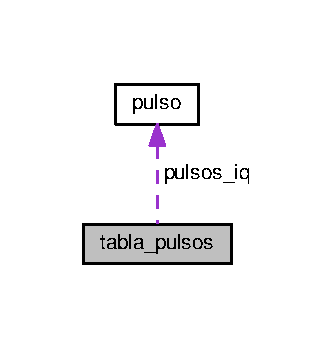
\includegraphics[width=161pt]{structtabla__pulsos__coll__graph}
\end{center}
\end{figure}
\subsection*{Data Fields}
\begin{DoxyCompactItemize}
\item 
uint16\+\_\+t {\bf valid\+Samples}
\item 
struct {\bf pulso} {\bf pulsos\+\_\+iq} [$\,$]
\end{DoxyCompactItemize}


\subsection{Field Documentation}
\index{tabla\+\_\+pulsos@{tabla\+\_\+pulsos}!pulsos\+\_\+iq@{pulsos\+\_\+iq}}
\index{pulsos\+\_\+iq@{pulsos\+\_\+iq}!tabla\+\_\+pulsos@{tabla\+\_\+pulsos}}
\subsubsection[{pulsos\+\_\+iq}]{\setlength{\rightskip}{0pt plus 5cm}struct {\bf pulso} pulsos\+\_\+iq}\label{structtabla__pulsos_a127fdeb6df16b8c86d77eb90f1a09113}
\index{tabla\+\_\+pulsos@{tabla\+\_\+pulsos}!valid\+Samples@{valid\+Samples}}
\index{valid\+Samples@{valid\+Samples}!tabla\+\_\+pulsos@{tabla\+\_\+pulsos}}
\subsubsection[{valid\+Samples}]{\setlength{\rightskip}{0pt plus 5cm}uint16\+\_\+t valid\+Samples}\label{structtabla__pulsos_a3ee39c4c3a761ca1fe094dfc0723ec11}


The documentation for this struct was generated from the following file\+:\begin{DoxyCompactItemize}
\item 
openmp/{\bf main.\+c}\end{DoxyCompactItemize}

\chapter{File Documentation}
\section{html/dynsections.js File Reference}
\label{dynsections_8js}\index{html/dynsections.\+js@{html/dynsections.\+js}}
\subsection*{Functions}
\begin{DoxyCompactItemize}
\item 
function {\bf toggle\+Visibility} (link\+Obj)
\item 
function {\bf update\+Stripes} ()
\item 
function {\bf toggle\+Level} (level)
\item 
function {\bf toggle\+Folder} (id)
\item 
function {\bf toggle\+Inherit} (id)
\end{DoxyCompactItemize}


\subsection{Function Documentation}
\index{dynsections.\+js@{dynsections.\+js}!toggle\+Folder@{toggle\+Folder}}
\index{toggle\+Folder@{toggle\+Folder}!dynsections.\+js@{dynsections.\+js}}
\subsubsection[{toggle\+Folder(id)}]{\setlength{\rightskip}{0pt plus 5cm}function toggle\+Folder (
\begin{DoxyParamCaption}
\item[{}]{id}
\end{DoxyParamCaption}
)}\label{dynsections_8js_af244da4527af2d845dca04f5656376cd}
\index{dynsections.\+js@{dynsections.\+js}!toggle\+Inherit@{toggle\+Inherit}}
\index{toggle\+Inherit@{toggle\+Inherit}!dynsections.\+js@{dynsections.\+js}}
\subsubsection[{toggle\+Inherit(id)}]{\setlength{\rightskip}{0pt plus 5cm}function toggle\+Inherit (
\begin{DoxyParamCaption}
\item[{}]{id}
\end{DoxyParamCaption}
)}\label{dynsections_8js_ac057b640b17ff32af11ced151c9305b4}
\index{dynsections.\+js@{dynsections.\+js}!toggle\+Level@{toggle\+Level}}
\index{toggle\+Level@{toggle\+Level}!dynsections.\+js@{dynsections.\+js}}
\subsubsection[{toggle\+Level(level)}]{\setlength{\rightskip}{0pt plus 5cm}function toggle\+Level (
\begin{DoxyParamCaption}
\item[{}]{level}
\end{DoxyParamCaption}
)}\label{dynsections_8js_a19f577cc1ba571396a85bb1f48bf4df2}
\index{dynsections.\+js@{dynsections.\+js}!toggle\+Visibility@{toggle\+Visibility}}
\index{toggle\+Visibility@{toggle\+Visibility}!dynsections.\+js@{dynsections.\+js}}
\subsubsection[{toggle\+Visibility(link\+Obj)}]{\setlength{\rightskip}{0pt plus 5cm}function toggle\+Visibility (
\begin{DoxyParamCaption}
\item[{}]{link\+Obj}
\end{DoxyParamCaption}
)}\label{dynsections_8js_a1922c462474df7dfd18741c961d59a25}
\index{dynsections.\+js@{dynsections.\+js}!update\+Stripes@{update\+Stripes}}
\index{update\+Stripes@{update\+Stripes}!dynsections.\+js@{dynsections.\+js}}
\subsubsection[{update\+Stripes()}]{\setlength{\rightskip}{0pt plus 5cm}function update\+Stripes (
\begin{DoxyParamCaption}
{}
\end{DoxyParamCaption}
)}\label{dynsections_8js_a8f7493ad859d4fbf2523917511ee7177}

\section{html/jquery.js File Reference}
\label{jquery_8js}\index{html/jquery.\+js@{html/jquery.\+js}}
\subsection*{Functions}
\begin{DoxyCompactItemize}
\item 
{\bf b} {\bf extend} (\{css\+Hooks\+:\{opacity\+:\{get\+:function(bw, bv)\{{\bf if}(bv)\{var e={\bf Z}(bw,\char`\"{}opacity\char`\"{},\char`\"{}opacity\char`\"{});return e===\char`\"{}\char`\"{}?\char`\"{}1\char`\"{}\+:e\}else\{return bw.\+style.\+opacity\}\}\}\}, css\+Number\+:\{fill\+Opacity\+:true, font\+Weight\+:true, line\+Height\+:true, opacity\+:true, orphans\+:true, widows\+:true, z\+Index\+:true, zoom\+:true\}, css\+Props\+:\{\char`\"{}float\char`\"{}\+:b.\+support.\+css\+Float?\char`\"{}css\+Float\char`\"{}\+:\char`\"{}style\+Float\char`\"{}\}, style\+:function(bx, bw, bD, by)\{{\bf if}(!bx$\vert$$\vert$bx.\+node\+Type===3$\vert$$\vert$bx.\+node\+Type===8$\vert$$\vert$!bx.\+style)\{return\}var bB, bC, bz=b.\+camel\+Case(bw), bv=bx.\+style, bE=b.\+css\+Hooks[bz];bw=b.\+css\+Props[bz]$\vert$$\vert$bz;{\bf if}(b\+D!=={\bf L})\{bC=typeof bD;{\bf if}(bC===\char`\"{}string\char`\"{}\&\&(bB=I.\+exec(bD)))\{bD=(+(bB[1]+1)$\ast$+bB[2])+parse\+Float({\bf b.\+css}(bx, bw));bC=\char`\"{}number\char`\"{}\}if(bD==null$\vert$$\vert$bC===\char`\"{}number\char`\"{}\&\&is\+NaN(bD))\{return\}{\bf if}(bC===\char`\"{}number\char`\"{}\&\&!b.\+css\+Number[bz])\{bD+=\char`\"{}px\char`\"{}\}if(!bE$\vert$$\vert$!(\char`\"{}set\char`\"{}in bE)$\vert$$\vert$(bD=b\+E.\+set(bx, bD))!=={\bf L})\{try\{bv[bw]=bD\}catch(bA)\{\}\}\}else\{{\bf if}(bE \&\&\char`\"{}get\char`\"{}in bE \&\&(bB=b\+E.\+get(bx, false, by))!=={\bf L})\{return bB\}return bv[bw]\}\}, css\+:function(by, bx, bv)\{var bw, e;bx=b.\+camel\+Case(bx);e=b.\+css\+Hooks[bx];bx=b.\+css\+Props[bx]$\vert$$\vert$bx;{\bf if}(bx===\char`\"{}css\+Float\char`\"{})\{bx=\char`\"{}float\char`\"{}\}if(e \&\&\char`\"{}get\char`\"{}in e \&\&(bw=e.\+get(by, true, bv))!=={\bf L})\{return bw\}else\{{\bf if}({\bf Z})\{return {\bf Z}(by, bx)\}\}\}, swap\+:function(bx, bw, by)\{var e=\{\};for(var bv in bw)\{e[bv]=bx.\+style[bv];bx.\+style[bv]=bw[bv]\}by.\+call(bx);for(bv in bw)\{bx.\+style[bv]=e[bv]\}\}\})
\item 
{\bf b} {\bf each} ([\char`\"{}height\char`\"{},\char`\"{}width\char`\"{}], function(bv, e)\{b.\+css\+Hooks[e]=\{get\+:function(by, bx, bw)\{var bz;{\bf if}(bx)\{{\bf if}(by.\+offset\+Width!==0)\{return {\bf p}(by, e, bw)\}else\{b.\+swap(by, a7, function()\{bz={\bf p}(by, e, bw)\})\}return bz\}\}, set\+:function(bw, bx)\{{\bf if}(bc.\+test(bx))\{bx=parse\+Float(bx);{\bf if}(bx $>$=0)\{return bx+\char`\"{}px\char`\"{}\}\}else\{return bx\}\}\}\})
\item 
{\bf if} (!b.\+support.\+opacity)
\item 
{\bf b} (function()\{{\bf if}(!b.\+support.\+reliable\+Margin\+Right)\{b.\+css\+Hooks.\+margin\+Right=\{get\+:function(bw, bv)\{var e;b.\+swap(bw,\{display\+:\char`\"{}inline-\/block\char`\"{}\}, function()\{{\bf if}(bv)\{e={\bf Z}(bw,\char`\"{}margin-\/right\char`\"{},\char`\"{}margin\+Right\char`\"{})\}else\{e=bw.\+style.\+margin\+Right\}\});return e\}\}\}\})
\item 
{\bf if} (av.\+default\+View \&\&av.\+default\+View.\+get\+Computed\+Style)
\item 
{\bf if} (av.\+document\+Element.\+current\+Style)
\item 
function {\bf p} (by, bw, bv)
\item 
{\bf if} (b.\+expr \&\&b.\+expr.\+filters)
\end{DoxyCompactItemize}
\subsection*{Variables}
\begin{DoxyCompactItemize}
\item 
function {\bf bb}
\item 
function {\bf L} \{var av=bb.\+document,bu=bb.\+navigator,bl=bb.\+location
\item 
var {\bf b}
\item 
var {\bf au} =/opacity=([$^\wedge$)]$\ast$)/,z=/([A-\/{\bf Z}]$\vert$$^\wedge$ms)/g,bc=/$^\wedge$-\/?\textbackslash{}d+(?\+:px)?\$/i,bn=/$^\wedge$-\/?\textbackslash{}d/,I=/$^\wedge$([\textbackslash{}-\/+])=([\textbackslash{}-\/+.\textbackslash{}de]+)/,a7=\{position\+:\char`\"{}absolute\char`\"{},visibility\+:\char`\"{}hidden\char`\"{},display\+:\char`\"{}block\char`\"{}\},an=[\char`\"{}Left\char`\"{},\char`\"{}Right\char`\"{}],a1=[\char`\"{}Top\char`\"{},\char`\"{}Bottom\char`\"{}],Z,aI,aX
\item 
{\bf b} fn {\bf css} =function(e,bv)\{{\bf if}(arguments.\+length===2\&\&bv==={\bf L})\{return this\}return b.\+access(this,e,bv,true,function(bx,bw,by)\{return by!=={\bf L}?b.\+style(bx,bw,by)\+:b.\+css(bx,bw)\})\}
\item 
{\bf b} {\bf cur\+C\+SS} ={\bf b.\+css}
\item 
{\bf Z} =aI$\vert$$\vert$aX
\item 
var {\bf k} =/\%20/g
\item 
var {\bf ap} =/\textbackslash{}[\textbackslash{}]\$/
\item 
var {\bf bs} =/\textbackslash{}r?\textbackslash{}n/g
\item 
var {\bf bq} =/\#.$\ast$\$/
\item 
var {\bf aD} =/$^\wedge$(.$\ast$?)\+:[ \textbackslash{}t]$\ast$([$^\wedge$\textbackslash{}r\textbackslash{}n]$\ast$)\textbackslash{}r?\$/mg
\item 
var {\bf aZ} =/$^\wedge$(?\+:color$\vert$date$\vert$datetime$\vert$datetime-\/local$\vert$email$\vert$hidden$\vert$month$\vert$number$\vert$password$\vert$range$\vert$search$\vert$tel$\vert$text$\vert$time$\vert$url$\vert$week)\$/i
\item 
var {\bf aM} =/$^\wedge$(?\+:about$\vert$app$\vert$app\textbackslash{}-\/storage$\vert$.+\textbackslash{}-\/extension$\vert$file$\vert$res$\vert$widget)\+:\$/
\item 
var {\bf aQ} =/$^\wedge$(?\+:G\+ET$\vert$H\+E\+AD)\$/
\item 
var {\bf c}
\end{DoxyCompactItemize}


\subsection{Function Documentation}
\index{jquery.\+js@{jquery.\+js}!b@{b}}
\index{b@{b}!jquery.\+js@{jquery.\+js}}
\subsubsection[{b(function()\lcurly{}if("!b.\+support.\+reliable\+Margin\+Right)\lcurly{}b.\+css\+Hooks.\+margin\+Right=\lcurly{}get\+:function(bw, bv)\lcurly{}var e;b.\+swap(bw,\lcurly{}display\+:""inline-\/block""\rcurly{}, function()\lcurly{}if(bv)\lcurly{}e=\+Z(bw,""margin-\/right"",""margin\+Right"")\rcurly{}else\lcurly{}e=bw.\+style.\+margin\+Right\rcurly{}\rcurly{});return e\rcurly{}\rcurly{}\rcurly{}\rcurly{})}]{\setlength{\rightskip}{0pt plus 5cm}b (
\begin{DoxyParamCaption}
\item[{function()\{{\bf if}(!b.\+support.\+reliable\+Margin\+Right)\{b.\+css\+Hooks.\+margin\+Right=\{get\+:function(bw, bv)\{var e;b.\+swap(bw,\{display\+:\char`\"{}inline-\/block\char`\"{}\}, function()\{{\bf if}(bv)\{e={\bf Z}(bw,\char`\"{}margin-\/right\char`\"{},\char`\"{}margin\+Right\char`\"{})\}else\{e=bw.\+style.\+margin\+Right\}\});return e\}\}\}\}}]{}
\end{DoxyParamCaption}
)}\label{jquery_8js_a2fa551895933fae935a0a6b87282241d}
\index{jquery.\+js@{jquery.\+js}!each@{each}}
\index{each@{each}!jquery.\+js@{jquery.\+js}}
\subsubsection[{each([""height"",""width""], function(bv, e)\lcurly{}b.\+css\+Hooks[e]=\lcurly{}get\+:function(by, bx, bw)\lcurly{}var bz;if(bx)\lcurly{}if(by.\+offset\+Width"!==0)\lcurly{}return p(by, e, bw)\rcurly{}else\lcurly{}b.\+swap(by, a7, function()\lcurly{}bz=p(by, e, bw)\rcurly{})\rcurly{}return bz\rcurly{}\rcurly{}, set\+:function(bw, bx)\lcurly{}if(bc.\+test(bx))\lcurly{}bx=parse\+Float(bx);if(bx $>$=0)\lcurly{}return bx+""px""\rcurly{}\rcurly{}else\lcurly{}return bx\rcurly{}\rcurly{}\rcurly{}\rcurly{})}]{\setlength{\rightskip}{0pt plus 5cm}{\bf b} each (
\begin{DoxyParamCaption}
\item[{function(bv, e)\{b.\+css\+Hooks[e]=\{get\+:function(by, bx, bw)\{var bz;{\bf if}(bx)\{{\bf if}(by.\+offset\+Width!==0)\{return {\bf p}(by, e, bw)\}else\{b.\+swap(by, a7, function()\{bz={\bf p}(by, e, bw)\})\}return bz\}\}, set\+:function(bw, bx)\{{\bf if}(bc.\+test(bx))\{bx=parse\+Float(bx);{\bf if}(bx $>$=0)\{return bx+\char`\"{}px\char`\"{}\}\}else\{return bx\}\}\}\}}]{}
\end{DoxyParamCaption}
)}\label{jquery_8js_a871ff39db627c54c710a3e9909b8234c}
\index{jquery.\+js@{jquery.\+js}!extend@{extend}}
\index{extend@{extend}!jquery.\+js@{jquery.\+js}}
\subsubsection[{extend(\lcurly{}css\+Hooks\+:\lcurly{}opacity\+:\lcurly{}get\+:function(bw, bv)\lcurly{}if(bv)\lcurly{}var e=\+Z(bw,""opacity"",""opacity"");return e===""""?""1""\+:e\rcurly{}else\lcurly{}return bw.\+style.\+opacity\rcurly{}\rcurly{}\rcurly{}\rcurly{}, css\+Number\+:\lcurly{}fill\+Opacity\+:true, font\+Weight\+:true, line\+Height\+:true, opacity\+:true, orphans\+:true, widows\+:true, z\+Index\+:true, zoom\+:true\rcurly{}, css\+Props\+:\lcurly{}""float""\+:b.\+support.\+css\+Float?""css\+Float""\+:""style\+Float""\rcurly{}, style\+:function(bx, bw, b\+D, by)\lcurly{}if("!bx\texttt{"|}\texttt{"|}bx.\+node\+Type===3\texttt{"|}\texttt{"|}bx.\+node\+Type===8\texttt{"|}\texttt{"|}"!bx.\+style)\lcurly{}return\rcurly{}var b\+B, b\+C, bz=b.\+camel\+Case(bw), bv=bx.\+style, b\+E=b.\+css\+Hooks[bz];bw=b.\+css\+Props[bz]\texttt{"|}\texttt{"|}bz;if(bD"!==\+L)\lcurly{}b\+C=typeof b\+D;if(b\+C===""string""\&\&(b\+B=\+I.\+exec(b\+D)))\lcurly{}b\+D=(+(bB[1]+1)$\ast$+bB[2])+parse\+Float(b.\+css(bx, bw));b\+C=""number""\rcurly{}if(b\+D==null\texttt{"|}\texttt{"|}b\+C===""number""\&\&is\+Na\+N(b\+D))\lcurly{}return\rcurly{}if(b\+C===""number""\&\&"!b.\+css\+Number[bz])\lcurly{}b\+D+=""px""\rcurly{}if("!bE\texttt{"|}\texttt{"|}"!(""set""in b\+E)\texttt{"|}\texttt{"|}(b\+D=b\+E.\+set(bx, b\+D))"!==\+L)\lcurly{}try\lcurly{}bv[bw]=bD\rcurly{}catch(b\+A)\lcurly{}\rcurly{}\rcurly{}\rcurly{}else\lcurly{}if(b\+E \&\&""get""in b\+E \&\&(b\+B=b\+E.\+get(bx, false, by))"!==\+L)\lcurly{}return bB\rcurly{}return bv[bw]\rcurly{}\rcurly{}, css\+:function(by, bx, bv)\lcurly{}var bw, e;bx=b.\+camel\+Case(bx);e=b.\+css\+Hooks[bx];bx=b.\+css\+Props[bx]\texttt{"|}\texttt{"|}bx;if(bx===""css\+Float"")\lcurly{}bx=""float""\rcurly{}if(e \&\&""get""in e \&\&(bw=e.\+get(by, true, bv))"!==\+L)\lcurly{}return bw\rcurly{}else\lcurly{}if(\+Z)\lcurly{}return Z(by, bx)\rcurly{}\rcurly{}\rcurly{}, swap\+:function(bx, bw, by)\lcurly{}var e=\lcurly{}\rcurly{};for(var bv in bw)\lcurly{}e[bv]=bx.\+style[bv];bx.\+style[bv]=bw[bv]\rcurly{}by.\+call(bx);for(bv in bw)\lcurly{}bx.\+style[bv]=e[bv]\rcurly{}\rcurly{}\rcurly{})}]{\setlength{\rightskip}{0pt plus 5cm}{\bf b} extend (
\begin{DoxyParamCaption}
\item[{\{css\+Hooks\+:\{opacity\+:\{get\+:function(bw, bv)\{{\bf if}(bv)\{var e={\bf Z}(bw,\char`\"{}opacity\char`\"{},\char`\"{}opacity\char`\"{});return e===\char`\"{}\char`\"{}?\char`\"{}1\char`\"{}\+:e\}else\{return bw.\+style.\+opacity\}\}\}\}, css\+Number\+:\{fill\+Opacity\+:true, font\+Weight\+:true, line\+Height\+:true, opacity\+:true, orphans\+:true, widows\+:true, z\+Index\+:true, zoom\+:true\}, css\+Props\+:\{\char`\"{}float\char`\"{}\+:b.\+support.\+css\+Float?\char`\"{}css\+Float\char`\"{}\+:\char`\"{}style\+Float\char`\"{}\}, style\+:function(bx, bw, bD, by)\{{\bf if}(!bx$\vert$$\vert$bx.\+node\+Type===3$\vert$$\vert$bx.\+node\+Type===8$\vert$$\vert$!bx.\+style)\{return\}var bB, bC, bz=b.\+camel\+Case(bw), bv=bx.\+style, bE=b.\+css\+Hooks[bz];bw=b.\+css\+Props[bz]$\vert$$\vert$bz;{\bf if}(b\+D!=={\bf L})\{bC=typeof bD;{\bf if}(bC===\char`\"{}string\char`\"{}\&\&(bB=I.\+exec(bD)))\{bD=(+(bB[1]+1)$\ast$+bB[2])+parse\+Float({\bf b.\+css}(bx, bw));bC=\char`\"{}number\char`\"{}\}if(bD==null$\vert$$\vert$bC===\char`\"{}number\char`\"{}\&\&is\+NaN(bD))\{return\}{\bf if}(bC===\char`\"{}number\char`\"{}\&\&!b.\+css\+Number[bz])\{bD+=\char`\"{}px\char`\"{}\}if(!bE$\vert$$\vert$!(\char`\"{}set\char`\"{}in bE)$\vert$$\vert$(bD=b\+E.\+set(bx, bD))!=={\bf L})\{try\{bv[bw]=bD\}catch(bA)\{\}\}\}else\{{\bf if}(bE \&\&\char`\"{}get\char`\"{}in bE \&\&(bB=b\+E.\+get(bx, false, by))!=={\bf L})\{return bB\}return bv[bw]\}\}, css\+:function(by, bx, bv)\{var bw, e;bx=b.\+camel\+Case(bx);e=b.\+css\+Hooks[bx];bx=b.\+css\+Props[bx]$\vert$$\vert$bx;{\bf if}(bx===\char`\"{}css\+Float\char`\"{})\{bx=\char`\"{}float\char`\"{}\}if(e \&\&\char`\"{}get\char`\"{}in e \&\&(bw=e.\+get(by, true, bv))!=={\bf L})\{return bw\}else\{{\bf if}({\bf Z})\{return {\bf Z}(by, bx)\}\}\}, swap\+:function(bx, bw, by)\{var e=\{\};for(var bv in bw)\{e[bv]=bx.\+style[bv];bx.\+style[bv]=bw[bv]\}by.\+call(bx);for(bv in bw)\{bx.\+style[bv]=e[bv]\}\}\}}]{}
\end{DoxyParamCaption}
)}\label{jquery_8js_a5fb206c91c64d1be35fde236706eab86}
\index{jquery.\+js@{jquery.\+js}!if@{if}}
\index{if@{if}!jquery.\+js@{jquery.\+js}}
\subsubsection[{if(av.\+document\+Element.\+current\+Style)}]{\setlength{\rightskip}{0pt plus 5cm}if (
\begin{DoxyParamCaption}
\item[{av.\+document\+Element.}]{current\+Style}
\end{DoxyParamCaption}
)}\label{jquery_8js_a2c54bd8ed7482e89d19331ba61fe221c}
\index{jquery.\+js@{jquery.\+js}!if@{if}}
\index{if@{if}!jquery.\+js@{jquery.\+js}}
\subsubsection[{if(av.\+default\+View \&\&av.\+default\+View.\+get\+Computed\+Style)}]{\setlength{\rightskip}{0pt plus 5cm}if (
\begin{DoxyParamCaption}
\item[{av.\+default\+View \&\&av.\+default\+View.}]{get\+Computed\+Style}
\end{DoxyParamCaption}
)}\label{jquery_8js_a30d3d2cd5b567c9f31b2aa30b9cb3bb8}
\index{jquery.\+js@{jquery.\+js}!if@{if}}
\index{if@{if}!jquery.\+js@{jquery.\+js}}
\subsubsection[{if(b.\+expr \&\&b.\+expr.\+filters)}]{\setlength{\rightskip}{0pt plus 5cm}if (
\begin{DoxyParamCaption}
\item[{b.\+expr \&\&b.\+expr.}]{filters}
\end{DoxyParamCaption}
)}\label{jquery_8js_a42cbfadee2b4749e8f699ea8d745a0e4}
\index{jquery.\+js@{jquery.\+js}!if@{if}}
\index{if@{if}!jquery.\+js@{jquery.\+js}}
\subsubsection[{if("!b.\+support.\+opacity)}]{\setlength{\rightskip}{0pt plus 5cm}if (
\begin{DoxyParamCaption}
\item[{!b.\+support.}]{opacity}
\end{DoxyParamCaption}
)}\label{jquery_8js_a9db6d45a025ad692282fe23e69eeba43}
\index{jquery.\+js@{jquery.\+js}!p@{p}}
\index{p@{p}!jquery.\+js@{jquery.\+js}}
\subsubsection[{p(by, bw, bv)}]{\setlength{\rightskip}{0pt plus 5cm}function p (
\begin{DoxyParamCaption}
\item[{}]{by, }
\item[{}]{bw, }
\item[{}]{bv}
\end{DoxyParamCaption}
)}\label{jquery_8js_a2335e57f79b6acfb6de59c235dc8a83e}


\subsection{Variable Documentation}
\index{jquery.\+js@{jquery.\+js}!aD@{aD}}
\index{aD@{aD}!jquery.\+js@{jquery.\+js}}
\subsubsection[{aD}]{\setlength{\rightskip}{0pt plus 5cm}var aD =/$^\wedge$(.$\ast$?)\+:[ \textbackslash{}t]$\ast$([$^\wedge$\textbackslash{}r\textbackslash{}n]$\ast$)\textbackslash{}r?\$/mg}\label{jquery_8js_ad223f5fba68c41c1236671ac5c5b0fcb}
\index{jquery.\+js@{jquery.\+js}!aM@{aM}}
\index{aM@{aM}!jquery.\+js@{jquery.\+js}}
\subsubsection[{aM}]{\setlength{\rightskip}{0pt plus 5cm}var aM =/$^\wedge$(?\+:about$\vert$app$\vert$app\textbackslash{}-\/storage$\vert$.+\textbackslash{}-\/extension$\vert$file$\vert$res$\vert$widget)\+:\$/}\label{jquery_8js_a8cc6111a5def3ea889157d13fb9a9672}
\index{jquery.\+js@{jquery.\+js}!ap@{ap}}
\index{ap@{ap}!jquery.\+js@{jquery.\+js}}
\subsubsection[{ap}]{\setlength{\rightskip}{0pt plus 5cm}var ap =/\textbackslash{}[\textbackslash{}]\$/}\label{jquery_8js_a6ddf393cc7f9a8828e197bb0d9916c44}
\index{jquery.\+js@{jquery.\+js}!aQ@{aQ}}
\index{aQ@{aQ}!jquery.\+js@{jquery.\+js}}
\subsubsection[{aQ}]{\setlength{\rightskip}{0pt plus 5cm}var aQ =/$^\wedge$(?\+:G\+ET$\vert$H\+E\+AD)\$/}\label{jquery_8js_a79eb58dc6cdf0aef563d5dc1ded27df5}
\index{jquery.\+js@{jquery.\+js}!au@{au}}
\index{au@{au}!jquery.\+js@{jquery.\+js}}
\subsubsection[{au}]{\setlength{\rightskip}{0pt plus 5cm}var au =/opacity=([$^\wedge$)]$\ast$)/,z=/([A-\/{\bf Z}]$\vert$$^\wedge$ms)/g,bc=/$^\wedge$-\/?\textbackslash{}d+(?\+:px)?\$/i,bn=/$^\wedge$-\/?\textbackslash{}d/,I=/$^\wedge$([\textbackslash{}-\/+])=([\textbackslash{}-\/+.\textbackslash{}de]+)/,a7=\{position\+:\char`\"{}absolute\char`\"{},visibility\+:\char`\"{}hidden\char`\"{},display\+:\char`\"{}block\char`\"{}\},an=[\char`\"{}Left\char`\"{},\char`\"{}Right\char`\"{}],a1=[\char`\"{}Top\char`\"{},\char`\"{}Bottom\char`\"{}],Z,aI,aX}\label{jquery_8js_a4fd8ddfab07c8d7c7cae0ab0e052cad3}
\index{jquery.\+js@{jquery.\+js}!aZ@{aZ}}
\index{aZ@{aZ}!jquery.\+js@{jquery.\+js}}
\subsubsection[{aZ}]{\setlength{\rightskip}{0pt plus 5cm}var aZ =/$^\wedge$(?\+:color$\vert$date$\vert$datetime$\vert$datetime-\/local$\vert$email$\vert$hidden$\vert$month$\vert$number$\vert$password$\vert$range$\vert$search$\vert$tel$\vert$text$\vert$time$\vert$url$\vert$week)\$/i}\label{jquery_8js_ac87125cdee1a5e57da4ef619af49bc7d}
\index{jquery.\+js@{jquery.\+js}!b@{b}}
\index{b@{b}!jquery.\+js@{jquery.\+js}}
\subsubsection[{b}]{\setlength{\rightskip}{0pt plus 5cm}var b}\label{jquery_8js_aa4026ad5544b958e54ce5e106fa1c805}
{\bfseries Initial value\+:}
\begin{DoxyCode}
=(\textcolor{keyword}{function}()\{var bF=\textcolor{keyword}{function}(b0,b1)\{\textcolor{keywordflow}{return} \textcolor{keyword}{new} bF.fn.init(b0,b1,bD)\},bU=bb.jQuery,bH=
      bb.$,bD,bY=/^(?:[^#<]*(<[\(\backslash\)w\(\backslash\)W]+>)[^>]*$|#([\(\backslash\)w\(\backslash\)-]*)$)/,bM=/\(\backslash\)S/,bI=/^\(\backslash\)s+/,bE=/\(\backslash\)s+$/,bA=/^<(\(\backslash\)w+)\(\backslash\)s*\(\backslash\)/?>(?:<\(\backslash\)/\(\backslash\)
      1>)?$/,bN=/^[\(\backslash\)],:\{\}\(\backslash\)s]*$/,bW=/\(\backslash\)\(\backslash\)(?:[\textcolor{stringliteral}{"\(\backslash\)\(\backslash\)\(\backslash\)/bfnrt]|u[0-9a-fA-F]\{4\})/g,bP=/"}[^\textcolor{stringliteral}{"\(\backslash\)\(\backslash\)\(\backslash\)n\(\backslash\)r]*"}|\textcolor{keyword}{true}|\textcolor{keyword}{false}|null|-?\(\backslash\)d+(?
      :\(\backslash\).\(\backslash\)d*)?(?:[eE][+\(\backslash\)-]?\(\backslash\)d+)?/g,bJ=/(?:^|:|,)(?:\(\backslash\)s*\(\backslash\)[)+/g,by=/(webkit)[ \(\backslash\)/]([\(\backslash\)w.]+)/,bR=/(opera)(?:.*version)?[
       \(\backslash\)/]([\(\backslash\)w.]+)/,bQ=/(msie) ([\(\backslash\)w.]+)/,bS=/(mozilla)(?:.*? rv:([\(\backslash\)w.]+))?/,bB=/-([a-z]|[0-9])/ig,bZ=/^-ms-/,bT=\textcolor{keyword}{
      function}(b0,b1)\{\textcolor{keywordflow}{return}(b1+\textcolor{stringliteral}{""}).toUpperCase()\},bX=bu.userAgent,bV,bC,e,bL=Object.prototype.toString,bG=Object.
      prototype.hasOwnProperty,bz=Array.prototype.push,bK=Array.prototype.slice,bO=String.prototype.trim,bv=Array.
      prototype.indexOf,bx=\{\};bF.fn=bF.prototype=\{constructor:bF,init:\textcolor{keyword}{function}(b0,b4,b3)\{var b2,b5,b1,b6;\textcolor{keywordflow}{if}(!b0)\{\textcolor{keywordflow}{
      return} \textcolor{keyword}{this}\}\textcolor{keywordflow}{if}(b0.nodeType)\{this.context=\textcolor{keyword}{this}[0]=b0;this.length=1;\textcolor{keywordflow}{return} \textcolor{keyword}{this}\}\textcolor{keywordflow}{if}(b0===\textcolor{stringliteral}{"body"}&&!b4&&av.body)\{
      this.context=av;\textcolor{keyword}{this}[0]=av.body;this.selector=b0;this.length=1;\textcolor{keywordflow}{return} \textcolor{keyword}{this}\}\textcolor{keywordflow}{if}(typeof b0===\textcolor{stringliteral}{"string"})\{\textcolor{keywordflow}{if}(b0.
      charAt(0)===\textcolor{stringliteral}{"<"}&&b0.charAt(b0.length-1)===\textcolor{stringliteral}{">"}&&b0.length>=3)\{b2=[null,b0,null]\}\textcolor{keywordflow}{else}\{b2=bY.exec(b0)\}\textcolor{keywordflow}{if}(b2&&(b2[1]
      ||!b4))\{\textcolor{keywordflow}{if}(b2[1])\{b4=b4 instanceof bF?b4[0]:b4;b6=(b4?b4.ownerDocument||b4:av);b1=bA.exec(b0);\textcolor{keywordflow}{if}(b1)\{\textcolor{keywordflow}{if}(bF.
      isPlainObject(b4))\{b0=[av.createElement(b1[1])];bF.fn.attr.call(b0,b4,\textcolor{keyword}{true})\}\textcolor{keywordflow}{else}\{b0=[b6.createElement(b1[1])]\}
      \}\textcolor{keywordflow}{else}\{b1=bF.buildFragment([b2[1]],[b6]);b0=(b1.cacheable?bF.clone(b1.fragment):b1.fragment).childNodes\}\textcolor{keywordflow}{
      return} bF.merge(\textcolor{keyword}{this},b0)\}\textcolor{keywordflow}{else}\{b5=av.getElementById(b2[2]);\textcolor{keywordflow}{if}(b5&&b5.parentNode)\{\textcolor{keywordflow}{if}(b5.id!==b2[2])\{\textcolor{keywordflow}{return} b3.find(
      b0)\}this.length=1;\textcolor{keyword}{this}[0]=b5\}this.context=av;this.selector=b0;\textcolor{keywordflow}{return} \textcolor{keyword}{this}\}\}\textcolor{keywordflow}{else}\{\textcolor{keywordflow}{if}(!b4||b4.jquery)\{\textcolor{keywordflow}{return}(b4
      ||b3).find(b0)\}\textcolor{keywordflow}{else}\{\textcolor{keywordflow}{return} this.constructor(b4).find(b0)\}\}\}\textcolor{keywordflow}{else}\{\textcolor{keywordflow}{if}(bF.isFunction(b0))\{\textcolor{keywordflow}{return} b3.ready(b0)\}\}\textcolor{keywordflow}{
      if}(b0.selector!==L)\{this.selector=b0.selector;this.context=b0.context\}\textcolor{keywordflow}{return} bF.makeArray(b0,\textcolor{keyword}{this})\},selector:\textcolor{stringliteral}{
      ""},jquery:\textcolor{stringliteral}{"1.7.1"},length:0,size:\textcolor{keyword}{function}()\{\textcolor{keywordflow}{return} this.length\},toArray:\textcolor{keyword}{function}()\{\textcolor{keywordflow}{return} bK.call(\textcolor{keyword}{this},0)\},\textcolor{keyword}{
      get}:\textcolor{keyword}{function}(b0)\{\textcolor{keywordflow}{return} b0==null?this.toArray():(b0<0?this[this.length+b0]:this[b0])\},pushStack:function(b1,b3
      ,b0)\{var b2=this.constructor();\textcolor{keywordflow}{if}(bF.isArray(b1))\{bz.apply(b2,b1)\}\textcolor{keywordflow}{else}\{bF.merge(b2,b1)\}b2.prevObject=\textcolor{keyword}{this};b2
      .context=this.context;\textcolor{keywordflow}{if}(b3===\textcolor{stringliteral}{"find"})\{b2.selector=this.selector+(this.selector?\textcolor{stringliteral}{" "}:\textcolor{stringliteral}{""})+b0\}\textcolor{keywordflow}{else}\{\textcolor{keywordflow}{if}(b3)\{b2.
      selector=this.selector+\textcolor{stringliteral}{"."}+b3+\textcolor{stringliteral}{"("}+b0+\textcolor{stringliteral}{")"}\}\}\textcolor{keywordflow}{return} b2\},each:\textcolor{keyword}{function}(b1,b0)\{\textcolor{keywordflow}{return} bF.each(\textcolor{keyword}{this},b1,b0)\},ready:\textcolor{keyword}{
      function}(b0)\{bF.bindReady();bC.add(b0);\textcolor{keywordflow}{return} \textcolor{keyword}{this}\},eq:\textcolor{keyword}{function}(b0)\{b0=+b0;\textcolor{keywordflow}{return} b0===-1?this.slice(b0):this.
      slice(b0,b0+1)\},first:function()\{\textcolor{keywordflow}{return} this.eq(0)\},last:\textcolor{keyword}{function}()\{\textcolor{keywordflow}{return} this.eq(-1)\},slice:\textcolor{keyword}{function}()\{\textcolor{keywordflow}{
      return} this.pushStack(bK.apply(\textcolor{keyword}{this},arguments),\textcolor{stringliteral}{"slice"},bK.call(arguments).join(\textcolor{stringliteral}{","}))\},map:\textcolor{keyword}{function}(b0)\{\textcolor{keywordflow}{return} 
      this.pushStack(bF.map(\textcolor{keyword}{this},\textcolor{keyword}{function}(b2,b1)\{return b0.call(b2,b1,b2)\}))\},end:\textcolor{keyword}{function}()\{\textcolor{keywordflow}{return} this.prevObject|
      |this.constructor(null)\},push:bz,sort:[].sort,splice:[].splice\};bF.fn.init.prototype=bF.fn;bF.extend=bF.fn.
      extend=\textcolor{keyword}{function}()\{var b9,b2,b0,b1,b6,b7,b5=arguments[0]||\{\},b4=1,b3=arguments.length,b8=\textcolor{keyword}{false};\textcolor{keywordflow}{if}(typeof b5===\textcolor{stringliteral}{
      "boolean"})\{b8=b5;b5=arguments[1]||\{\};b4=2\}\textcolor{keywordflow}{if}(typeof b5!==\textcolor{stringliteral}{"object"}&&!bF.isFunction(b5))\{b5=\{\}\}\textcolor{keywordflow}{if}(b3===b4)\{b5=\textcolor{keyword}{
      this};--b4\}\textcolor{keywordflow}{for}(;b4<b3;b4++)\{\textcolor{keywordflow}{if}((b9=arguments[b4])!=null)\{\textcolor{keywordflow}{for}(b2 in b9)\{b0=b5[b2];b1=b9[b2];\textcolor{keywordflow}{if}(b5===b1)\{\textcolor{keywordflow}{
      continue}\}\textcolor{keywordflow}{if}(b8&&b1&&(bF.isPlainObject(b1)||(b6=bF.isArray(b1))))\{\textcolor{keywordflow}{if}(b6)\{b6=\textcolor{keyword}{false};b7=b0&&bF.isArray(b0)?b0:[]\}\textcolor{keywordflow}{else}\{
      b7=b0&&bF.isPlainObject(b0)?b0:\{\}\}b5[b2]=bF.extend(b8,b7,b1)\}\textcolor{keywordflow}{else}\{\textcolor{keywordflow}{if}(b1!==L)\{b5[b2]=b1\}\}\}\}\}\textcolor{keywordflow}{return} b5\};bF.
      extend(\{noConflict:\textcolor{keyword}{function}(b0)\{\textcolor{keywordflow}{if}(bb.$===bF)\{bb.$=bH\}\textcolor{keywordflow}{if}(b0&&bb.jQuery===bF)\{bb.jQuery=bU\}\textcolor{keywordflow}{return} bF\},isReady:\textcolor{keyword}{
      false},readyWait:1,holdReady:\textcolor{keyword}{function}(b0)\{\textcolor{keywordflow}{if}(b0)\{bF.readyWait++\}\textcolor{keywordflow}{else}\{bF.ready(\textcolor{keyword}{true})\}\},ready:\textcolor{keyword}{function}(b0)\{\textcolor{keywordflow}{if}((b0
      ===\textcolor{keyword}{true}&&!--bF.readyWait)||(b0!==\textcolor{keyword}{true}&&!bF.isReady))\{\textcolor{keywordflow}{if}(!av.body)\{\textcolor{keywordflow}{return} setTimeout(bF.ready,1)\}bF.isReady=\textcolor{keyword}{
      true};\textcolor{keywordflow}{if}(b0!==\textcolor{keyword}{true}&&--bF.readyWait>0)\{\textcolor{keywordflow}{return}\}bC.fireWith(av,[bF]);\textcolor{keywordflow}{if}(bF.fn.trigger)\{bF(av).trigger(\textcolor{stringliteral}{"ready"}).
      off(\textcolor{stringliteral}{"ready"})\}\}\},bindReady:\textcolor{keyword}{function}()\{\textcolor{keywordflow}{if}(bC)\{\textcolor{keywordflow}{return}\}bC=bF.Callbacks(\textcolor{stringliteral}{"once memory"});\textcolor{keywordflow}{if}(av.readyState===\textcolor{stringliteral}{"complete
      "})\{\textcolor{keywordflow}{return} setTimeout(bF.ready,1)\}\textcolor{keywordflow}{if}(av.addEventListener)\{av.addEventListener(\textcolor{stringliteral}{"DOMContentLoaded"},e,\textcolor{keyword}{false});
      bb.addEventListener(\textcolor{stringliteral}{"load"},bF.ready,\textcolor{keyword}{false})\}\textcolor{keywordflow}{else}\{\textcolor{keywordflow}{if}(av.attachEvent)\{av.attachEvent(\textcolor{stringliteral}{"onreadystatechange"},e);
      bb.attachEvent(\textcolor{stringliteral}{"onload"},bF.ready);var b0=\textcolor{keyword}{false};\textcolor{keywordflow}{try}\{b0=bb.frameElement==null\}\textcolor{keywordflow}{catch}(b1)\{\}\textcolor{keywordflow}{if}(av.
      documentElement.doScroll&&b0)\{bw()\}\}\}\},isFunction:\textcolor{keyword}{function}(b0)\{\textcolor{keywordflow}{return} bF.type(b0)===\textcolor{stringliteral}{"function"}\},isArray:Array.isArray||\textcolor{keyword}{
      function}(b0)\{\textcolor{keywordflow}{return} bF.type(b0)===\textcolor{stringliteral}{"array"}\},isWindow:\textcolor{keyword}{function}(b0)\{\textcolor{keywordflow}{return} b0&&typeof b0===\textcolor{stringliteral}{"object"}&&\textcolor{stringliteral}{"setInterval"}
       in b0\},isNumeric:\textcolor{keyword}{function}(b0)\{\textcolor{keywordflow}{return} !isNaN(parseFloat(b0))&&isFinite(b0)\},type:\textcolor{keyword}{function}(b0)\{\textcolor{keywordflow}{return} b0==
      null?String(b0):bx[bL.call(b0)]||\textcolor{stringliteral}{"object"}\},isPlainObject:function(b2)\{\textcolor{keywordflow}{if}(!b2||bF.type(b2)!==\textcolor{stringliteral}{"object"}||b2.
      nodeType||bF.isWindow(b2))\{\textcolor{keywordflow}{return} \textcolor{keyword}{false}\}\textcolor{keywordflow}{try}\{\textcolor{keywordflow}{if}(b2.constructor&&!bG.call(b2,\textcolor{stringliteral}{"constructor"})&&!bG.call(b2.constructor
      .prototype,\textcolor{stringliteral}{"isPrototypeOf"}))\{\textcolor{keywordflow}{return} \textcolor{keyword}{false}\}\}\textcolor{keywordflow}{catch}(b1)\{\textcolor{keywordflow}{return} \textcolor{keyword}{false}\}var b0;\textcolor{keywordflow}{for}(b0 in b2)\{\}\textcolor{keywordflow}{return} b0===
      L||bG.call(b2,b0)\},isEmptyObject:\textcolor{keyword}{function}(b1)\{\textcolor{keywordflow}{for}(var b0 in b1)\{\textcolor{keywordflow}{return} \textcolor{keyword}{false}\}\textcolor{keywordflow}{return} \textcolor{keyword}{true}\},error:\textcolor{keyword}{function}(b0
      )\{\textcolor{keywordflow}{throw} \textcolor{keyword}{new} Error(b0)\},parseJSON:\textcolor{keyword}{function}(b0)\{\textcolor{keywordflow}{if}(typeof b0!==\textcolor{stringliteral}{"string"}||!b0)\{\textcolor{keywordflow}{return} null\}b0=bF.trim(b0);\textcolor{keywordflow}{if}(
      bb.JSON&&bb.JSON.parse)\{\textcolor{keywordflow}{return} bb.JSON.parse(b0)\}\textcolor{keywordflow}{if}(bN.test(b0.replace(bW,\textcolor{stringliteral}{"@"}).replace(bP,\textcolor{stringliteral}{"]"}).replace(bJ,\textcolor{stringliteral}{"
      "})))\{\textcolor{keywordflow}{return}(\textcolor{keyword}{new} Function(\textcolor{stringliteral}{"return "}+b0))()\}bF.error(\textcolor{stringliteral}{"Invalid JSON: "}+b0)\},parseXML:\textcolor{keyword}{function}(b2)\{var b0,b1;\textcolor{keywordflow}{try}
      \{\textcolor{keywordflow}{if}(bb.DOMParser)\{b1=\textcolor{keyword}{new} DOMParser();b0=b1.parseFromString(b2,\textcolor{stringliteral}{"text/xml"})\}\textcolor{keywordflow}{else}\{b0=\textcolor{keyword}{new} ActiveXObject(\textcolor{stringliteral}{"
      Microsoft.XMLDOM"});b0.async=\textcolor{stringliteral}{"false"};b0.loadXML(b2)\}\}\textcolor{keywordflow}{catch}(b3)\{b0=L\}\textcolor{keywordflow}{if}(!b0||!b0.documentElement||b0.
      getElementsByTagName(\textcolor{stringliteral}{"parsererror"}).length)\{bF.error(\textcolor{stringliteral}{"Invalid XML: "}+b2)\}\textcolor{keywordflow}{return} b0\},noop:\textcolor{keyword}{function}()\{\},globalEval:\textcolor{keyword}{function}(b0
      )\{\textcolor{keywordflow}{if}(b0&&bM.test(b0))\{(bb.execScript||\textcolor{keyword}{function}(b1)\{bb[\textcolor{stringliteral}{"eval"}].call(bb,b1)\})(b0)\}\},camelCase:\textcolor{keyword}{function}(b0)\{\textcolor{keywordflow}{
      return} b0.replace(bZ,\textcolor{stringliteral}{"ms-"}).replace(bB,bT)\},nodeName:\textcolor{keyword}{function}(b1,b0)\{\textcolor{keywordflow}{return} b1.nodeName&&b1.nodeName.
      toUpperCase()===b0.toUpperCase()\},each:\textcolor{keyword}{function}(b3,b6,b2)\{var b1,b4=0,b5=b3.length,b0=b5===
      L||bF.isFunction(b3);\textcolor{keywordflow}{if}(b2)\{\textcolor{keywordflow}{if}(b0)\{\textcolor{keywordflow}{for}(b1 in b3)\{\textcolor{keywordflow}{if}(b6.apply(b3[b1],b2)===\textcolor{keyword}{false})\{\textcolor{keywordflow}{break}\}\}\}\textcolor{keywordflow}{else}\{\textcolor{keywordflow}{for}(;b4<b5;)\{\textcolor{keywordflow}{
      if}(b6.apply(b3[b4++],b2)===\textcolor{keyword}{false})\{\textcolor{keywordflow}{break}\}\}\}\}\textcolor{keywordflow}{else}\{\textcolor{keywordflow}{if}(b0)\{\textcolor{keywordflow}{for}(b1 in b3)\{\textcolor{keywordflow}{if}(b6.call(b3[b1],b1,b3[b1])===\textcolor{keyword}{false})\{\textcolor{keywordflow}{
      break}\}\}\}\textcolor{keywordflow}{else}\{\textcolor{keywordflow}{for}(;b4<b5;)\{\textcolor{keywordflow}{if}(b6.call(b3[b4],b4,b3[b4++])===\textcolor{keyword}{false})\{\textcolor{keywordflow}{break}\}\}\}\}\textcolor{keywordflow}{return} b3\},trim:bO?\textcolor{keyword}{function}(b0)\{\textcolor{keywordflow}{
      return} b0==null?\textcolor{stringliteral}{""}:bO.call(b0)\}:\textcolor{keyword}{function}(b0)\{\textcolor{keywordflow}{return} b0==null?\textcolor{stringliteral}{""}:b0.toString().replace(bI,\textcolor{stringliteral}{""}).replace(bE,\textcolor{stringliteral}{""})\},
      makeArray:\textcolor{keyword}{function}(b3,b1)\{var b0=b1||[];\textcolor{keywordflow}{if}(b3!=null)\{var b2=bF.type(b3);\textcolor{keywordflow}{if}(b3.length==null||b2===\textcolor{stringliteral}{"string"}||b2
      ===\textcolor{stringliteral}{"function"}||b2===\textcolor{stringliteral}{"regexp"}||bF.isWindow(b3))\{bz.call(b0,b3)\}\textcolor{keywordflow}{else}\{bF.merge(b0,b3)\}\}\textcolor{keywordflow}{return} b0\},inArray:\textcolor{keyword}{
      function}(b2,b3,b1)\{var b0;\textcolor{keywordflow}{if}(b3)\{\textcolor{keywordflow}{if}(bv)\{\textcolor{keywordflow}{return} bv.call(b3,b2,b1)\}b0=b3.length;b1=b1?b1<0?Math.max(0,b0+b1):b1:0;\textcolor{keywordflow}{
      for}(;b1<b0;b1++)\{\textcolor{keywordflow}{if}(b1 in b3&&b3[b1]===b2)\{\textcolor{keywordflow}{return} b1\}\}\}\textcolor{keywordflow}{return} -1\},merge:\textcolor{keyword}{function}(b4,b2)\{var b3=b4.length,b1=0
      ;\textcolor{keywordflow}{if}(typeof b2.length===\textcolor{stringliteral}{"number"})\{\textcolor{keywordflow}{for}(var b0=b2.length;b1<b0;b1++)\{b4[b3++]=b2[b1]\}\}\textcolor{keywordflow}{else}\{\textcolor{keywordflow}{while}(b2[b1]!==
      L)\{b4[b3++]=b2[b1++]\}\}b4.length=b3;\textcolor{keywordflow}{return} b4\},grep:\textcolor{keyword}{function}(b1,b6,b0)\{var b2=[],b5;b0=!!b0;\textcolor{keywordflow}{for}(var b3=0,b4=
      b1.length;b3<b4;b3++)\{b5=!!b6(b1[b3],b3);\textcolor{keywordflow}{if}(b0!==b5)\{b2.push(b1[b3])\}\}\textcolor{keywordflow}{return} b2\},map:\textcolor{keyword}{function}(b0,b7,b8)\{var 
      b5,b6,b4=[],b2=0,b1=b0.length,b3=b0 instanceof bF||b1!==L&&typeof b1===\textcolor{stringliteral}{"number"}&&((b1>0&&b0[0]&&b0[b1-1])||
      b1===0||bF.isArray(b0));\textcolor{keywordflow}{if}(b3)\{\textcolor{keywordflow}{for}(;b2<b1;b2++)\{b5=b7(b0[b2],b2,b8);\textcolor{keywordflow}{if}(b5!=null)\{b4[b4.length]=b5\}\}\}\textcolor{keywordflow}{else}\{\textcolor{keywordflow}{for}(
      b6 in b0)\{b5=b7(b0[b6],b6,b8);\textcolor{keywordflow}{if}(b5!=null)\{b4[b4.length]=b5\}\}\}\textcolor{keywordflow}{return} b4.concat.apply([],b4)\},guid:1,proxy:\textcolor{keyword}{
      function}(b4,b3)\{\textcolor{keywordflow}{if}(typeof b3===\textcolor{stringliteral}{"string"})\{var b2=b4[b3];b3=b4;b4=b2\}\textcolor{keywordflow}{if}(!bF.isFunction(b4))\{\textcolor{keywordflow}{return} 
      L\}var b0=bK.call(arguments,2),b1=\textcolor{keyword}{function}()\{\textcolor{keywordflow}{return} b4.apply(b3,b0.concat(bK.call(arguments)))\};b1.guid=b4.
      guid=b4.guid||b1.guid||bF.guid++;\textcolor{keywordflow}{return} b1\},access:\textcolor{keyword}{function}(b0,b8,b6,b2,b5,b7)\{var b1=b0.length;\textcolor{keywordflow}{if}(typeof b8
      ===\textcolor{stringliteral}{"object"})\{\textcolor{keywordflow}{for}(var b3 in b8)\{bF.access(b0,b3,b8[b3],b2,b5,b6)\}\textcolor{keywordflow}{return} b0\}\textcolor{keywordflow}{if}(b6!==
      L)\{b2=!b7&&b2&&bF.isFunction(b6);\textcolor{keywordflow}{for}(var b4=0;b4<b1;b4++)\{b5(b0[b4],b8,b2?b6.call(b0[b4],b4,b5(b0[b4],b8)):
      b6,b7)\}\textcolor{keywordflow}{return} b0\}\textcolor{keywordflow}{return} b1?b5(b0[0],b8):L\},now:function()\{\textcolor{keywordflow}{return}(\textcolor{keyword}{new} Date()).getTime()\},uaMatch:\textcolor{keyword}{function}(b1)
      \{b1=b1.toLowerCase();var b0=by.exec(b1)||bR.exec(b1)||bQ.exec(b1)||b1.indexOf(\textcolor{stringliteral}{"compatible"})<0&&bS.exec(b1)||
      [];\textcolor{keywordflow}{return}\{browser:b0[1]||\textcolor{stringliteral}{""},version:b0[2]||\textcolor{stringliteral}{"0"}\}\},sub:\textcolor{keyword}{function}()\{\textcolor{keyword}{function} b0(b3,b4)\{\textcolor{keywordflow}{return} \textcolor{keyword}{new} b0.fn.init(b3,
      b4)\}bF.extend(\textcolor{keyword}{true},b0,\textcolor{keyword}{this});b0.superclass=\textcolor{keyword}{this};b0.fn=b0.prototype=\textcolor{keyword}{this}();b0.fn.constructor=b0;b0.sub=this.
      sub;b0.fn.init=\textcolor{keyword}{function} b2(b3,b4)\{\textcolor{keywordflow}{if}(b4&&b4 instanceof bF&&!(b4 instanceof b0))\{b4=b0(b4)\}\textcolor{keywordflow}{return} bF.fn.init.
      call(\textcolor{keyword}{this},b3,b4,b1)\};b0.fn.init.prototype=b0.fn;var b1=b0(av);\textcolor{keywordflow}{return} b0\},browser:\{\}\});bF.each(\textcolor{stringliteral}{"Boolean Number
       String Function Array Date RegExp Object"}.split(\textcolor{stringliteral}{" "}),\textcolor{keyword}{function}(b1,b0)\{bx[\textcolor{stringliteral}{"[object "}+b0+\textcolor{stringliteral}{"]"}]=b0.toLowerCase()\}
      );bV=bF.uaMatch(bX);\textcolor{keywordflow}{if}(bV.browser)\{bF.browser[bV.browser]=\textcolor{keyword}{true};bF.browser.version=bV.version\}\textcolor{keywordflow}{if}(bF.browser.
      webkit)\{bF.browser.safari=\textcolor{keyword}{true}\}\textcolor{keywordflow}{if}(bM.test(\textcolor{stringliteral}{"\(\backslash\)xA0"}))\{bI=/^[\(\backslash\)s\(\backslash\)xA0]+/;bE=/[\(\backslash\)s\(\backslash\)xA0]+$/\}bD=bF(av);\textcolor{keywordflow}{if}(av.
      addEventListener)\{e=\textcolor{keyword}{function}()\{av.removeEventListener(\textcolor{stringliteral}{"DOMContentLoaded"},e,\textcolor{keyword}{false});bF.ready()\}\}\textcolor{keywordflow}{else}\{\textcolor{keywordflow}{if}(av.attachEvent)\{
      e=\textcolor{keyword}{function}()\{\textcolor{keywordflow}{if}(av.readyState===\textcolor{stringliteral}{"complete"})\{av.detachEvent(\textcolor{stringliteral}{"onreadystatechange"},e);bF.ready()\}\}\}\}\textcolor{keyword}{function} bw
      ()\{\textcolor{keywordflow}{if}(bF.isReady)\{\textcolor{keywordflow}{return}\}\textcolor{keywordflow}{try}\{av.documentElement.doScroll(\textcolor{stringliteral}{"left"})\}\textcolor{keywordflow}{catch}(b0)\{setTimeout(bw,1);\textcolor{keywordflow}{return}\}bF.ready(
      )\}\textcolor{keywordflow}{return} bF\})();var a2=\{\};\textcolor{keyword}{function} X(e)\{var bv=a2[e]=\{\},bw,bx;e=e.split(/\(\backslash\)s+/);\textcolor{keywordflow}{for}(bw=0,bx=e.length;bw<bx;bw
      ++)\{bv[e[bw]]=\textcolor{keyword}{true}\}\textcolor{keywordflow}{return} bv\}b.Callbacks=\textcolor{keyword}{function}(bw)\{bw=bw?(a2[bw]||X(bw)):\{\};var bB=[],bC=[],bx,by,bv,bz,
      bA,bE=\textcolor{keyword}{function}(bF)\{var bG,bJ,bI,bH,bK;\textcolor{keywordflow}{for}(bG=0,bJ=bF.length;bG<bJ;bG++)\{bI=bF[bG];bH=
      b.type(bI);\textcolor{keywordflow}{if}(bH===\textcolor{stringliteral}{"array"})\{bE(bI)\}\textcolor{keywordflow}{else}\{\textcolor{keywordflow}{if}(bH===\textcolor{stringliteral}{"function"})\{\textcolor{keywordflow}{if}(!bw.unique||!bD.has(bI))\{bB.push(bI)\}\}\}\}\},e=\textcolor{keyword}{
      function}(bG,bF)\{bF=bF||[];bx=!bw.memory||[bG,bF];by=\textcolor{keyword}{true};bA=bv||0;bv=0;bz=bB.length;\textcolor{keywordflow}{for}(;bB&&bA<bz;bA++)\{\textcolor{keywordflow}{if}(
      bB[bA].apply(bG,bF)===\textcolor{keyword}{false}&&bw.stopOnFalse)\{bx=\textcolor{keyword}{true};\textcolor{keywordflow}{break}\}\}by=\textcolor{keyword}{false};\textcolor{keywordflow}{if}(bB)\{\textcolor{keywordflow}{if}(!bw.once)\{\textcolor{keywordflow}{if}(bC&&bC.length)\{
      bx=bC.shift();bD.fireWith(bx[0],bx[1])\}\}\textcolor{keywordflow}{else}\{\textcolor{keywordflow}{if}(bx===\textcolor{keyword}{true})\{bD.disable()\}\textcolor{keywordflow}{else}\{bB=[]\}\}\}\},bD=\{add:\textcolor{keyword}{function}()\{\textcolor{keywordflow}{if}(
      bB)\{var bF=bB.length;bE(arguments);\textcolor{keywordflow}{if}(by)\{bz=bB.length\}\textcolor{keywordflow}{else}\{\textcolor{keywordflow}{if}(bx&&bx!==\textcolor{keyword}{true})\{bv=bF;e(bx[0],bx[1])\}\}\}\textcolor{keywordflow}{return} \textcolor{keyword}{
      this}\},\textcolor{keyword}{remove}:\textcolor{keyword}{function}()\{\textcolor{keywordflow}{if}(bB)\{var bF=arguments,bH=0,bI=bF.length;\textcolor{keywordflow}{for}(;bH<bI;bH++)\{\textcolor{keywordflow}{for}(var bG=0;bG<bB.length
      ;bG++)\{\textcolor{keywordflow}{if}(bF[bH]===bB[bG])\{\textcolor{keywordflow}{if}(by)\{\textcolor{keywordflow}{if}(bG<=bz)\{bz--;\textcolor{keywordflow}{if}(bG<=bA)\{bA--\}\}\}bB.splice(bG--,1);\textcolor{keywordflow}{if}(bw.unique)\{\textcolor{keywordflow}{break}\}\}\}
      \}\}\textcolor{keywordflow}{return} \textcolor{keyword}{this}\},has:\textcolor{keyword}{function}(bG)\{\textcolor{keywordflow}{if}(bB)\{var bF=0,bH=bB.length;\textcolor{keywordflow}{for}(;bF<bH;bF++)\{\textcolor{keywordflow}{if}(bG===bB[bF])\{\textcolor{keywordflow}{return} \textcolor{keyword}{true}\}\}\}\textcolor{keywordflow}{
      return} \textcolor{keyword}{false}\},empty:\textcolor{keyword}{function}()\{bB=[];\textcolor{keywordflow}{return} \textcolor{keyword}{this}\},disable:\textcolor{keyword}{function}()\{bB=bC=bx=L;\textcolor{keywordflow}{return} \textcolor{keyword}{this}\},disabled:\textcolor{keyword}{
      function}()\{\textcolor{keywordflow}{return} !bB\},lock:\textcolor{keyword}{function}()\{bC=L;\textcolor{keywordflow}{if}(!bx||bx===\textcolor{keyword}{true})\{bD.disable()\}\textcolor{keywordflow}{return} \textcolor{keyword}{this}\},locked:\textcolor{keyword}{function}()\{\textcolor{keywordflow}{return} 
      !bC\},fireWith:\textcolor{keyword}{function}(bG,bF)\{\textcolor{keywordflow}{if}(bC)\{\textcolor{keywordflow}{if}(by)\{\textcolor{keywordflow}{if}(!bw.once)\{bC.push([bG,bF])\}\}\textcolor{keywordflow}{else}\{\textcolor{keywordflow}{if}(!(bw.once&&bx))\{e(bG,bF)\}
      \}\}\textcolor{keywordflow}{return} \textcolor{keyword}{this}\},fire:\textcolor{keyword}{function}()\{bD.fireWith(\textcolor{keyword}{this},arguments);\textcolor{keywordflow}{return} \textcolor{keyword}{this}\},fired:\textcolor{keyword}{function}()\{\textcolor{keywordflow}{return} !!bx\}\};\textcolor{keywordflow}{
      return} bD\};var aJ=[].slice;b.extend(\{Deferred:\textcolor{keyword}{function}(by)\{var bx=b.Callbacks(\textcolor{stringliteral}{"once memory"}),bw=
      b.Callbacks(\textcolor{stringliteral}{"once memory"}),bv=b.Callbacks(\textcolor{stringliteral}{"memory"}),e=\textcolor{stringliteral}{"pending"},bA=\{resolve:bx,reject:bw,notify:bv\},bC=\{
      done:bx.add,fail:bw.add,progress:bv.add,state:\textcolor{keyword}{function}()\{\textcolor{keywordflow}{return} e\},isResolved:bx.fired,isRejected:bw.fired,then
      :\textcolor{keyword}{function}(bE,bD,bF)\{bB.done(bE).fail(bD).progress(bF);\textcolor{keywordflow}{return} \textcolor{keyword}{this}\},always:\textcolor{keyword}{function}()\{bB.done.apply(bB,
      arguments).fail.apply(bB,arguments);\textcolor{keywordflow}{return} \textcolor{keyword}{this}\},pipe:\textcolor{keyword}{function}(bF,bE,bD)\{\textcolor{keywordflow}{return} b.Deferred(\textcolor{keyword}{function}(bG)\{
      b.each(\{done:[bF,\textcolor{stringliteral}{"resolve"}],fail:[bE,\textcolor{stringliteral}{"reject"}],progress:[bD,\textcolor{stringliteral}{"notify"}]\},\textcolor{keyword}{function}(bI,bL)\{var bH=bL[0],bK=bL[1
      ],bJ;\textcolor{keywordflow}{if}(b.isFunction(bH))\{bB[bI](\textcolor{keyword}{function}()\{bJ=bH.apply(\textcolor{keyword}{this},arguments);\textcolor{keywordflow}{if}(bJ&&b.isFunction(bJ.promise))\{bJ.
      promise().then(bG.resolve,bG.reject,bG.notify)\}\textcolor{keywordflow}{else}\{bG[bK+\textcolor{stringliteral}{"With"}](\textcolor{keyword}{this}===bB?bG:\textcolor{keyword}{this},[bJ])\}\})\}\textcolor{keywordflow}{else}\{bB[bI](bG[
      bK])\}\})\}).promise()\},promise:\textcolor{keyword}{function}(bE)\{\textcolor{keywordflow}{if}(bE==null)\{bE=bC\}\textcolor{keywordflow}{else}\{\textcolor{keywordflow}{for}(var bD in bC)\{bE[bD]=bC[bD]\}\}\textcolor{keywordflow}{return} bE
      \}\},bB=bC.promise(\{\}),bz;\textcolor{keywordflow}{for}(bz in bA)\{bB[bz]=bA[bz].fire;bB[bz+\textcolor{stringliteral}{"With"}]=bA[bz].fireWith\}bB.done(\textcolor{keyword}{function}()\{e=\textcolor{stringliteral}{
      "resolved"}\},bw.disable,bv.lock).fail(\textcolor{keyword}{function}()\{e=\textcolor{stringliteral}{"rejected"}\},bx.disable,bv.lock);\textcolor{keywordflow}{if}(by)\{by.call(bB,bB)\}\textcolor{keywordflow}{
      return} bB\},when:\textcolor{keyword}{function}(bA)\{var bx=aJ.call(arguments,0),bv=0,e=bx.length,bB=\textcolor{keyword}{new} Array(e),bw=e,by=e,bC=e<=1&&bA&
      &b.isFunction(bA.promise)?bA:b.Deferred(),bE=bC.promise();\textcolor{keyword}{function} bD(bF)\{\textcolor{keywordflow}{return} \textcolor{keyword}{function}(bG)\{bx[bF]=
      arguments.length>1?aJ.call(arguments,0):bG;\textcolor{keywordflow}{if}(!(--bw))\{bC.resolveWith(bC,bx)\}\}\}\textcolor{keyword}{function} bz(bF)\{\textcolor{keywordflow}{return} \textcolor{keyword}{function}(bG)\{
      bB[bF]=arguments.length>1?aJ.call(arguments,0):bG;bC.notifyWith(bE,bB)\}\}\textcolor{keywordflow}{if}(e>1)\{\textcolor{keywordflow}{for}(;bv<e;bv++)\{\textcolor{keywordflow}{if}(bx[bv]&&
      bx[bv].promise&&b.isFunction(bx[bv].promise))\{bx[bv].promise().then(bD(bv),bC.reject,bz(bv))\}\textcolor{keywordflow}{else}\{--bw\}\}\textcolor{keywordflow}{if}(!
      bw)\{bC.resolveWith(bC,bx)\}\}\textcolor{keywordflow}{else}\{\textcolor{keywordflow}{if}(bC!==bA)\{bC.resolveWith(bC,e?[bA]:[])\}\}\textcolor{keywordflow}{return} bE\}\});
      b.support=(\textcolor{keyword}{function}()\{var bJ,bI,bF,bG,bx,bE,bA,bD,bz,bK,bB,by,bw,bv=av.createElement(\textcolor{stringliteral}{"div"}),bH=av.
      documentElement;bv.setAttribute(\textcolor{stringliteral}{"className"},\textcolor{stringliteral}{"t"});bv.innerHTML=\textcolor{stringliteral}{"   <link/><table></table><a href='/a'
       style='top:1px;float:left;opacity:.55;'>a</a><input type='checkbox'/>"};bI=bv.getElementsByTagName(\textcolor{stringliteral}{"*"});bF=bv.
      getElementsByTagName(\textcolor{stringliteral}{"a"})[0];\textcolor{keywordflow}{if}(!bI||!bI.length||!bF)\{\textcolor{keywordflow}{return}\{\}\}bG=av.createElement(\textcolor{stringliteral}{"select"});bx=bG.appendChild(av.
      createElement(\textcolor{stringliteral}{"option"}));bE=bv.getElementsByTagName(\textcolor{stringliteral}{"input"})[0];bJ=\{leadingWhitespace:(bv.firstChild.nodeType===3),
      tbody:!bv.getElementsByTagName(\textcolor{stringliteral}{"tbody"}).length,htmlSerialize:!!bv.getElementsByTagName(\textcolor{stringliteral}{"link"}).length,style:/
      top/.test(bF.getAttribute(\textcolor{stringliteral}{"style"})),hrefNormalized:(bF.getAttribute(\textcolor{stringliteral}{"href"})===\textcolor{stringliteral}{"/a"}),opacity:/^0.55/.test(bF.
      style.opacity),cssFloat:!!bF.style.cssFloat,checkOn:(bE.value===\textcolor{stringliteral}{"on"}),optSelected:bx.selected,getSetAttribute
      :bv.className!==\textcolor{stringliteral}{"t"},enctype:!!av.createElement(\textcolor{stringliteral}{"form"}).enctype,html5Clone:av.createElement(\textcolor{stringliteral}{"nav"}).cloneNode(\textcolor{keyword}{
      true}).outerHTML!==\textcolor{stringliteral}{"<:nav></:nav>"},submitBubbles:\textcolor{keyword}{true},changeBubbles:\textcolor{keyword}{true},focusinBubbles:\textcolor{keyword}{false},deleteExpando:\textcolor{keyword}{
      true},noCloneEvent:\textcolor{keyword}{true},inlineBlockNeedsLayout:\textcolor{keyword}{false},shrinkWrapBlocks:\textcolor{keyword}{false},reliableMarginRight:\textcolor{keyword}{true}\};bE.
      checked=\textcolor{keyword}{true};bJ.noCloneChecked=bE.cloneNode(\textcolor{keyword}{true}).checked;bG.disabled=\textcolor{keyword}{true};bJ.optDisabled=!bx.disabled;\textcolor{keywordflow}{try}\{\textcolor{keyword}{delete}
       bv.test\}\textcolor{keywordflow}{catch}(bC)\{bJ.deleteExpando=\textcolor{keyword}{false}\}\textcolor{keywordflow}{if}(!bv.addEventListener&&bv.attachEvent&&bv.fireEvent)\{bv.
      attachEvent(\textcolor{stringliteral}{"onclick"},\textcolor{keyword}{function}()\{bJ.noCloneEvent=\textcolor{keyword}{false}\});bv.cloneNode(\textcolor{keyword}{true}).fireEvent(\textcolor{stringliteral}{"onclick"})\}bE=av.createElement
      (\textcolor{stringliteral}{"input"});bE.value=\textcolor{stringliteral}{"t"};bE.setAttribute(\textcolor{stringliteral}{"type"},\textcolor{stringliteral}{"radio"});bJ.radioValue=bE.value===\textcolor{stringliteral}{"t"};bE.setAttribute(\textcolor{stringliteral}{"checked
      "},\textcolor{stringliteral}{"checked"});bv.appendChild(bE);bD=av.createDocumentFragment();bD.appendChild(bv.lastChild);bJ.checkClone=bD
      .cloneNode(\textcolor{keyword}{true}).cloneNode(\textcolor{keyword}{true}).lastChild.checked;bJ.appendChecked=bE.checked;bD.removeChild(bE);bD.
      appendChild(bv);bv.innerHTML=\textcolor{stringliteral}{""};\textcolor{keywordflow}{if}(bb.getComputedStyle)\{bA=av.createElement(\textcolor{stringliteral}{"div"});bA.style.width=\textcolor{stringliteral}{"0"};bA.style.
      marginRight=\textcolor{stringliteral}{"0"};bv.style.width=\textcolor{stringliteral}{"2px"};bv.appendChild(bA);bJ.reliableMarginRight=(parseInt((
      bb.getComputedStyle(bA,null)||\{marginRight:0\}).marginRight,10)||0)===0\}\textcolor{keywordflow}{if}(bv.attachEvent)\{\textcolor{keywordflow}{for}(by in \{submit
      :1,change:1,focusin:1\})\{bB=\textcolor{stringliteral}{"on"}+by;bw=(bB in bv);\textcolor{keywordflow}{if}(!bw)\{bv.setAttribute(bB,\textcolor{stringliteral}{"return;"});bw=(typeof bv[bB]===\textcolor{stringliteral}{"
      function"})\}bJ[by+\textcolor{stringliteral}{"Bubbles"}]=bw\}\}bD.removeChild(bv);bD=bG=bx=bA=bv=bE=null;b(\textcolor{keyword}{function}()\{var bM,bU,bV,bT,bN,bO
      ,bL,bS,bR,e,bP,bQ=av.getElementsByTagName(\textcolor{stringliteral}{"body"})[0];\textcolor{keywordflow}{if}(!bQ)\{\textcolor{keywordflow}{return}\}bL=1;bS=\textcolor{stringliteral}{"
      position:absolute;top:0;left:0;width:1px;height:1px;margin:0;"};bR=\textcolor{stringliteral}{"visibility:hidden;border:0;"};e=\textcolor{stringliteral}{"style='"}+bS+\textcolor{stringliteral}{"border:5px solid
       #000;padding:0;'"};bP=\textcolor{stringliteral}{"<div "}+e+\textcolor{stringliteral}{"><div></div></div><table "}+e+\textcolor{stringliteral}{" cellpadding='0'
       cellspacing='0'><tr><td></td></tr></table>"};bM=av.createElement(\textcolor{stringliteral}{"div"});bM.style.cssText=bR+\textcolor{stringliteral}{"width:0;height:0;position:static;top:0;margin-top:"}+bL+\textcolor{stringliteral}{
      "px"};bQ.insertBefore(bM,bQ.firstChild);bv=av.createElement(\textcolor{stringliteral}{"div"});bM.appendChild(bv);bv.innerHTML=\textcolor{stringliteral}{"
      <table><tr><td style='padding:0;border:0;display:none'></td><td>t</td></tr></table>"};bz=bv.getElementsByTagName(\textcolor{stringliteral}{"td"})
      ;bw=(bz[0].offsetHeight===0);bz[0].style.display=\textcolor{stringliteral}{""};bz[1].style.display=\textcolor{stringliteral}{"none"};bJ.reliableHiddenOffsets=bw&&
      (bz[0].offsetHeight===0);bv.innerHTML=\textcolor{stringliteral}{""};bv.style.width=bv.style.paddingLeft=\textcolor{stringliteral}{"1px"};
      b.boxModel=bJ.boxModel=bv.offsetWidth===2;\textcolor{keywordflow}{if}(typeof bv.style.zoom!==\textcolor{stringliteral}{"undefined"})\{bv.style.display=\textcolor{stringliteral}{"inline"};
      bv.style.zoom=1;bJ.inlineBlockNeedsLayout=(bv.offsetWidth===2);bv.style.display=\textcolor{stringliteral}{""};bv.innerHTML=\textcolor{stringliteral}{"<div
       style='width:4px;'></div>"};bJ.shrinkWrapBlocks=(bv.offsetWidth!==2)\}bv.style.cssText=bS+bR;bv.innerHTML=bP;bU=bv.
      firstChild;bV=bU.firstChild;bN=bU.nextSibling.firstChild.firstChild;bO=\{doesNotAddBorder:(bV.offsetTop!==5),
      doesAddBorderForTableAndCells:(bN.offsetTop===5)\};bV.style.position=\textcolor{stringliteral}{"fixed"};bV.style.top=\textcolor{stringliteral}{"20px"};bO.
      fixedPosition=(bV.offsetTop===20||bV.offsetTop===15);bV.style.position=bV.style.top=\textcolor{stringliteral}{""};bU.style.overflow=\textcolor{stringliteral}{"hidden"};bU.
      style.position=\textcolor{stringliteral}{"relative"};bO.subtractsBorderForOverflowNotVisible=(bV.offsetTop===-5);bO.
      doesNotIncludeMarginInBodyOffset=(bQ.offsetTop!==bL);bQ.removeChild(bM);bv=bM=null;b.extend(bJ,bO)\});\textcolor{keywordflow}{return} bJ\})();var aS=/^(?:\(\backslash\)
      \{.*\(\backslash\)\}|\(\backslash\)[.*\(\backslash\)])$/,aA=/([A-Z])/g;b.extend(\{cache:\{\},uuid:0,expando:\textcolor{stringliteral}{"jQuery"}+(b.fn.jquery+Math.random()).replace
      (/\(\backslash\)D/g,\textcolor{stringliteral}{""}),noData:\{embed:\textcolor{keyword}{true},\textcolor{keywordtype}{object}:\textcolor{stringliteral}{"clsid:D27CDB6E-AE6D-11cf-96B8-444553540000"},applet:\textcolor{keyword}{true}\},hasData:\textcolor{keyword}{
      function}(e)\{e=e.nodeType?b.cache[e[b.expando]]:e[b.expando];\textcolor{keywordflow}{return} !!e&&!S(e)\},data:\textcolor{keyword}{function}(bx,bv,bz,by)\{\textcolor{keywordflow}{if}(!
      b.acceptData(bx))\{\textcolor{keywordflow}{return}\}var bG,bA,bD,bE=b.expando,bC=typeof bv===\textcolor{stringliteral}{"string"},bF=bx.nodeType,e=bF?
      b.cache:bx,bw=bF?bx[bE]:bx[bE]&&bE,bB=bv===\textcolor{stringliteral}{"events"};\textcolor{keywordflow}{if}((!bw||!e[bw]||(!bB&&!by&&!e[bw].data))&&bC&&bz===
      L)\{\textcolor{keywordflow}{return}\}\textcolor{keywordflow}{if}(!bw)\{\textcolor{keywordflow}{if}(bF)\{bx[bE]=bw=++b.uuid\}\textcolor{keywordflow}{else}\{bw=bE\}\}\textcolor{keywordflow}{if}(!e[bw])\{e[bw]=\{\};\textcolor{keywordflow}{if}(!bF)\{e[bw].toJSON=
      b.noop\}\}\textcolor{keywordflow}{if}(typeof bv===\textcolor{stringliteral}{"object"}||typeof bv===\textcolor{stringliteral}{"function"})\{\textcolor{keywordflow}{if}(by)\{e[bw]=b.extend(e[bw],bv)\}\textcolor{keywordflow}{else}\{e[bw].data=
      b.extend(e[bw].data,bv)\}\}bG=bA=e[bw];\textcolor{keywordflow}{if}(!by)\{\textcolor{keywordflow}{if}(!bA.data)\{bA.data=\{\}\}bA=bA.data\}\textcolor{keywordflow}{if}(bz!==
      L)\{bA[b.camelCase(bv)]=bz\}\textcolor{keywordflow}{if}(bB&&!bA[bv])\{\textcolor{keywordflow}{return} bG.events\}\textcolor{keywordflow}{if}(bC)\{bD=bA[bv];\textcolor{keywordflow}{if}(bD==null)\{bD=bA[
      b.camelCase(bv)]\}\}\textcolor{keywordflow}{else}\{bD=bA\}\textcolor{keywordflow}{return} bD\},removeData:\textcolor{keyword}{function}(bx,bv,by)\{\textcolor{keywordflow}{if}(!b.acceptData(bx))\{\textcolor{keywordflow}{return}\}var bB,
      bA,bz,bC=b.expando,bD=bx.nodeType,e=bD?b.cache:bx,bw=bD?bx[bC]:bC;\textcolor{keywordflow}{if}(!e[bw])\{\textcolor{keywordflow}{return}\}\textcolor{keywordflow}{if}(bv)\{bB=by?e[bw]:e[bw].
      data;\textcolor{keywordflow}{if}(bB)\{\textcolor{keywordflow}{if}(!b.isArray(bv))\{\textcolor{keywordflow}{if}(bv in bB)\{bv=[bv]\}\textcolor{keywordflow}{else}\{bv=b.camelCase(bv);\textcolor{keywordflow}{if}(bv in bB)\{bv=[bv]\}\textcolor{keywordflow}{else}\{bv=bv.
      split(\textcolor{stringliteral}{" "})\}\}\}\textcolor{keywordflow}{for}(bA=0,bz=bv.length;bA<bz;bA++)\{\textcolor{keyword}{delete} bB[bv[bA]]\}\textcolor{keywordflow}{if}(!(by?S:b.isEmptyObject)(bB))\{\textcolor{keywordflow}{return}\}\}\}\textcolor{keywordflow}{if}
      (!by)\{\textcolor{keyword}{delete} e[bw].data;\textcolor{keywordflow}{if}(!S(e[bw]))\{\textcolor{keywordflow}{return}\}\}\textcolor{keywordflow}{if}(b.support.deleteExpando||!e.setInterval)\{\textcolor{keyword}{delete} e[bw]\}\textcolor{keywordflow}{else}\{
      e[bw]=null\}\textcolor{keywordflow}{if}(bD)\{\textcolor{keywordflow}{if}(b.support.deleteExpando)\{\textcolor{keyword}{delete} bx[bC]\}\textcolor{keywordflow}{else}\{\textcolor{keywordflow}{if}(bx.removeAttribute)\{bx.removeAttribute(
      bC)\}\textcolor{keywordflow}{else}\{bx[bC]=null\}\}\}\},\_data:\textcolor{keyword}{function}(bv,e,bw)\{\textcolor{keywordflow}{return} b.data(bv,e,bw,\textcolor{keyword}{true})\},acceptData:\textcolor{keyword}{function}(bv)\{\textcolor{keywordflow}{if}(bv.
      nodeName)\{var e=b.noData[bv.nodeName.toLowerCase()];\textcolor{keywordflow}{if}(e)\{\textcolor{keywordflow}{return} !(e===\textcolor{keyword}{true}||bv.getAttribute(\textcolor{stringliteral}{"classid"})!==e)\}
      \}\textcolor{keywordflow}{return} \textcolor{keyword}{true}\}\});b.fn.extend(\{data:\textcolor{keyword}{function}(by,bA)\{var bB,e,bw,bz=null;\textcolor{keywordflow}{if}(typeof by===\textcolor{stringliteral}{"undefined"})\{\textcolor{keywordflow}{if}(this.
      length)\{bz=b.data(\textcolor{keyword}{this}[0]);\textcolor{keywordflow}{if}(\textcolor{keyword}{this}[0].nodeType===1&&!b.\_data(\textcolor{keyword}{this}[0],\textcolor{stringliteral}{"parsedAttrs"}))\{e=\textcolor{keyword}{this}[0].attributes;\textcolor{keywordflow}{for}(
      var bx=0,bv=e.length;bx<bv;bx++)\{bw=e[bx].name;\textcolor{keywordflow}{if}(bw.indexOf(\textcolor{stringliteral}{"data-"})===0)\{bw=b.camelCase(bw.substring(5));
      a5(\textcolor{keyword}{this}[0],bw,bz[bw])\}\}b.\_data(\textcolor{keyword}{this}[0],\textcolor{stringliteral}{"parsedAttrs"},\textcolor{keyword}{true})\}\}\textcolor{keywordflow}{return} bz\}\textcolor{keywordflow}{else}\{\textcolor{keywordflow}{if}(typeof by===\textcolor{stringliteral}{"object"})\{\textcolor{keywordflow}{return} 
      this.each(\textcolor{keyword}{function}()\{b.data(\textcolor{keyword}{this},by)\})\}\}bB=by.split(\textcolor{stringliteral}{"."});bB[1]=bB[1]?\textcolor{stringliteral}{"."}+bB[1]:\textcolor{stringliteral}{""};\textcolor{keywordflow}{if}(bA===
      L)\{bz=this.triggerHandler(\textcolor{stringliteral}{"getData"}+bB[1]+\textcolor{stringliteral}{"!"},[bB[0]]);\textcolor{keywordflow}{if}(bz===L&&this.length)\{bz=
      b.data(\textcolor{keyword}{this}[0],by);bz=a5(\textcolor{keyword}{this}[0],by,bz)\}\textcolor{keywordflow}{return} bz===L&&bB[1]?this.data(bB[0]):bz\}else\{\textcolor{keywordflow}{return} this.
      each(\textcolor{keyword}{function}()\{var bC=b(\textcolor{keyword}{this}),bD=[bB[0],bA];bC.triggerHandler(\textcolor{stringliteral}{"setData"}+bB[1]+\textcolor{stringliteral}{"!"},bD);
      b.data(\textcolor{keyword}{this},by,bA);bC.triggerHandler(\textcolor{stringliteral}{"changeData"}+bB[1]+\textcolor{stringliteral}{"!"},bD)\})\}\},removeData:\textcolor{keyword}{function}(e)\{\textcolor{keywordflow}{return} this.
      each(\textcolor{keyword}{function}()\{b.removeData(\textcolor{keyword}{this},e)\})\}\});\textcolor{keyword}{function} a5(bx,bw,by)\{\textcolor{keywordflow}{if}(by===L&&bx.nodeType===1)\{var bv=\textcolor{stringliteral}{"data-"}+
      bw.replace(aA,\textcolor{stringliteral}{"-$1"}).toLowerCase();by=bx.getAttribute(bv);\textcolor{keywordflow}{if}(typeof by===\textcolor{stringliteral}{"string"})\{\textcolor{keywordflow}{try}\{by=by===\textcolor{stringliteral}{"true"}?\textcolor{keyword}{true}:
      by===\textcolor{stringliteral}{"false"}?\textcolor{keyword}{false}:by===\textcolor{stringliteral}{"null"}?null:b.isNumeric(by)?parseFloat(by):aS.test(by)?b.parseJSON(by):by\}catch(bz)\{\}
      b.data(bx,bw,by)\}\textcolor{keywordflow}{else}\{by=L\}\}\textcolor{keywordflow}{return} by\}\textcolor{keyword}{function} S(bv)\{\textcolor{keywordflow}{for}(var e in bv)\{\textcolor{keywordflow}{if}(e===\textcolor{stringliteral}{"data"}&&
      b.isEmptyObject(bv[e]))\{\textcolor{keywordflow}{continue}\}\textcolor{keywordflow}{if}(e!==\textcolor{stringliteral}{"toJSON"})\{\textcolor{keywordflow}{return} \textcolor{keyword}{false}\}\}\textcolor{keywordflow}{return} \textcolor{keyword}{true}\}\textcolor{keyword}{function} bi(by,bx,bA)\{var bw=bx
      +\textcolor{stringliteral}{"defer"},bv=bx+\textcolor{stringliteral}{"queue"},e=bx+\textcolor{stringliteral}{"mark"},bz=b.\_data(by,bw);\textcolor{keywordflow}{if}(bz&&(bA===\textcolor{stringliteral}{"queue"}||!b.\_data(by,bv))&&(bA===\textcolor{stringliteral}{"mark"}||!
      b.\_data(by,e)))\{setTimeout(\textcolor{keyword}{function}()\{\textcolor{keywordflow}{if}(!b.\_data(by,bv)&&!b.\_data(by,e))\{b.removeData(by,bw,\textcolor{keyword}{true});bz.fire(
      )\}\},0)\}\}b.extend(\{\_mark:function(bv,e)\{if(bv)\{e=(e||\textcolor{stringliteral}{"fx"})+\textcolor{stringliteral}{"mark"};b.\_data(bv,e,(b.\_data(bv,e)||0)+1)\}\},
      \_unmark:\textcolor{keyword}{function}(by,bx,bv)\{if(by!==true)\{bv=bx;bx=by;by=false\}\textcolor{keywordflow}{if}(bx)\{bv=bv||\textcolor{stringliteral}{"fx"};var e=bv+\textcolor{stringliteral}{"mark"},bw=by?0:((b.\_data
      (bx,e)||1)-1);if(bw)\{b.\_data(bx,e,bw)\}\textcolor{keywordflow}{else}\{b.removeData(bx,e,true);bi(bx,bv,\textcolor{stringliteral}{"mark"})\}\}\},queue:\textcolor{keyword}{function}(bv,e,
      bx)\{var bw;\textcolor{keywordflow}{if}(bv)\{e=(e||\textcolor{stringliteral}{"fx"})+\textcolor{stringliteral}{"queue"};bw=b.\_data(bv,e);\textcolor{keywordflow}{if}(bx)\{\textcolor{keywordflow}{if}(!bw||b.isArray(bx))\{bw=
      b.\_data(bv,e,b.makeArray(bx))\}\textcolor{keywordflow}{else}\{bw.push(bx)\}\}\textcolor{keywordflow}{return} bw||[]\}\},dequeue:\textcolor{keyword}{function}(by,bx)\{bx=bx||\textcolor{stringliteral}{"fx"};var bv=
      b.queue(by,bx),bw=bv.shift(),e=\{\};\textcolor{keywordflow}{if}(bw===\textcolor{stringliteral}{"inprogress"})\{bw=bv.shift()\}\textcolor{keywordflow}{if}(bw)\{\textcolor{keywordflow}{if}(bx===\textcolor{stringliteral}{"fx"})\{bv.unshift(\textcolor{stringliteral}{"
      inprogress"})\}b.\_data(by,bx+\textcolor{stringliteral}{".run"},e);bw.call(by,\textcolor{keyword}{function}()\{b.dequeue(by,bx)\},e)\}\textcolor{keywordflow}{if}(!bv.length)\{
      b.removeData(by,bx+\textcolor{stringliteral}{"queue "}+bx+\textcolor{stringliteral}{".run"},\textcolor{keyword}{true});bi(by,bx,\textcolor{stringliteral}{"queue"})\}\}\});b.fn.extend(\{queue:\textcolor{keyword}{function}(e,bv)\{\textcolor{keywordflow}{if}(
      typeof e!==\textcolor{stringliteral}{"string"})\{bv=e;e=\textcolor{stringliteral}{"fx"}\}\textcolor{keywordflow}{if}(bv===L)\{\textcolor{keywordflow}{return} b.queue(\textcolor{keyword}{this}[0],e)\}\textcolor{keywordflow}{return} this.
      each(\textcolor{keyword}{function}()\{var bw=b.queue(\textcolor{keyword}{this},e,bv);\textcolor{keywordflow}{if}(e===\textcolor{stringliteral}{"fx"}&&bw[0]!==\textcolor{stringliteral}{"inprogress"})\{b.dequeue(\textcolor{keyword}{this},e)\}\})\},dequeue:\textcolor{keyword}{
      function}(e)\{\textcolor{keywordflow}{return} this.each(\textcolor{keyword}{function}()\{b.dequeue(\textcolor{keyword}{this},e)\})\},delay:\textcolor{keyword}{function}(bv,e)\{bv=
      b.fx?b.fx.speeds[bv]||bv:bv;e=e||\textcolor{stringliteral}{"fx"};\textcolor{keywordflow}{return} this.queue(e,\textcolor{keyword}{function}(bx,bw)\{var by=setTimeout(bx,bv);bw.stop=\textcolor{keyword}{
      function}()\{clearTimeout(by)\}\})\},clearQueue:\textcolor{keyword}{function}(e)\{\textcolor{keywordflow}{return} this.queue(e||\textcolor{stringliteral}{"fx"},[])\},promise:\textcolor{keyword}{function}(bD,bw
      )\{\textcolor{keywordflow}{if}(typeof bD!==\textcolor{stringliteral}{"string"})\{bw=bD;bD=L\}bD=bD||\textcolor{stringliteral}{"fx"};var e=b.Deferred(),bv=\textcolor{keyword}{this},by=bv.length,bB=1,bz=bD+\textcolor{stringliteral}{"defer"}
      ,bA=bD+\textcolor{stringliteral}{"queue"},bC=bD+\textcolor{stringliteral}{"mark"},bx;\textcolor{keyword}{function} bE()\{\textcolor{keywordflow}{if}(!(--bB))\{e.resolveWith(bv,[bv])\}\}\textcolor{keywordflow}{while}(by--)\{\textcolor{keywordflow}{if}((bx=
      b.data(bv[by],bz,L,\textcolor{keyword}{true})||(b.data(bv[by],bA,L,\textcolor{keyword}{true})||b.data(bv[by],bC,L,\textcolor{keyword}{true}))&&
      b.data(bv[by],bz,b.Callbacks(\textcolor{stringliteral}{"once memory"}),\textcolor{keyword}{true})))\{bB++;bx.add(bE)\}\}bE();\textcolor{keywordflow}{return} e.promise()\}\});var aP=/[
      \(\backslash\)n\(\backslash\)t\(\backslash\)r]/g,af=/\(\backslash\)s+/,aU=/\(\backslash\)r/g,g=/^(?:button|input)$/i,D=/^(?:button|input|\textcolor{keywordtype}{object}|select|textarea)$/i,l=/^a(?:rea
      )?$/i,ao=/^(?:autofocus|autoplay|async|checked|controls|defer|disabled|hidden|loop|multiple|open|readonly|
      required|scoped|selected)$/i,F=b.support.getSetAttribute,be,aY,aF;b.fn.extend(\{attr:function(e,bv)\{return b.ac
      cess(this,e,bv,true,b.attr)\},removeAttr:\textcolor{keyword}{function}(e)\{return this.each(function()\{b.removeAttr(this,e)\})\},prop
      :\textcolor{keyword}{function}(e,bv)\{\textcolor{keywordflow}{return} b.access(\textcolor{keyword}{this},e,bv,\textcolor{keyword}{true},b.prop)\},removeProp:\textcolor{keyword}{function}(e)\{e=
      b.propFix[e]||e;\textcolor{keywordflow}{return} this.each(\textcolor{keyword}{function}()\{\textcolor{keywordflow}{try}\{\textcolor{keyword}{this}[e]=L;\textcolor{keyword}{delete} \textcolor{keyword}{this}[e]\}\textcolor{keywordflow}{catch}(bv)\{\}\})\},addClass:\textcolor{keyword}{function}(
      by)\{var bA,bw,bv,bx,bz,bB,e;\textcolor{keywordflow}{if}(b.isFunction(by))\{\textcolor{keywordflow}{return} this.each(\textcolor{keyword}{function}(bC)\{b(\textcolor{keyword}{this}).addClass(by.call(\textcolor{keyword}{this},
      bC,\textcolor{keyword}{this}.className))\})\}\textcolor{keywordflow}{if}(by&&typeof by===\textcolor{stringliteral}{"string"})\{bA=by.split(af);\textcolor{keywordflow}{for}(bw=0,bv=this.length;bw<bv;bw++)\{bx=\textcolor{keyword}{
      this}[bw];\textcolor{keywordflow}{if}(bx.nodeType===1)\{\textcolor{keywordflow}{if}(!bx.className&&bA.length===1)\{bx.className=by\}\textcolor{keywordflow}{else}\{bz=\textcolor{stringliteral}{" "}+bx.className+\textcolor{stringliteral}{" "};\textcolor{keywordflow}{for}
      (bB=0,e=bA.length;bB<e;bB++)\{\textcolor{keywordflow}{if}(!~bz.indexOf(\textcolor{stringliteral}{" "}+bA[bB]+\textcolor{stringliteral}{" "}))\{bz+=bA[bB]+\textcolor{stringliteral}{" "}\}\}bx.className=
      b.trim(bz)\}\}\}\}\textcolor{keywordflow}{return} \textcolor{keyword}{this}\},removeClass:\textcolor{keyword}{function}(bz)\{var bA,bw,bv,by,bx,bB,e;\textcolor{keywordflow}{if}(b.isFunction(bz))\{\textcolor{keywordflow}{return} 
      this.each(\textcolor{keyword}{function}(bC)\{b(\textcolor{keyword}{this}).removeClass(bz.call(\textcolor{keyword}{this},bC,\textcolor{keyword}{this}.className))\})\}\textcolor{keywordflow}{if}((bz&&typeof bz===\textcolor{stringliteral}{"string"})||bz
      ===L)\{bA=(bz||\textcolor{stringliteral}{""}).split(af);\textcolor{keywordflow}{for}(bw=0,bv=this.length;bw<bv;bw++)\{by=\textcolor{keyword}{this}[bw];\textcolor{keywordflow}{if}(by.nodeType===1&&by.className
      )\{\textcolor{keywordflow}{if}(bz)\{bx=(\textcolor{stringliteral}{" "}+by.className+\textcolor{stringliteral}{" "}).replace(aP,\textcolor{stringliteral}{" "});\textcolor{keywordflow}{for}(bB=0,e=bA.length;bB<e;bB++)\{bx=bx.replace(\textcolor{stringliteral}{" "}+bA[bB]+\textcolor{stringliteral}{
      " "},\textcolor{stringliteral}{" "})\}by.className=b.trim(bx)\}\textcolor{keywordflow}{else}\{by.className=\textcolor{stringliteral}{""}\}\}\}\}\textcolor{keywordflow}{return} \textcolor{keyword}{this}\},toggleClass:\textcolor{keyword}{function}(bx,bv)\{var bw=
      typeof bx,e=typeof bv===\textcolor{stringliteral}{"boolean"};\textcolor{keywordflow}{if}(b.isFunction(bx))\{\textcolor{keywordflow}{return} this.each(\textcolor{keyword}{function}(by)\{
      b(\textcolor{keyword}{this}).toggleClass(bx.call(\textcolor{keyword}{this},by,\textcolor{keyword}{this}.className,bv),bv)\})\}\textcolor{keywordflow}{return} this.each(\textcolor{keyword}{function}()\{\textcolor{keywordflow}{if}(bw===\textcolor{stringliteral}{"string"})\{
      var bA,bz=0,by=b(\textcolor{keyword}{this}),bB=bv,bC=bx.split(af);\textcolor{keywordflow}{while}((bA=bC[bz++]))\{bB=e?bB:!by.hasClass(bA);by[bB?\textcolor{stringliteral}{"addClass"}:\textcolor{stringliteral}{
      "removeClass"}](bA)\}\}\textcolor{keywordflow}{else}\{\textcolor{keywordflow}{if}(bw===\textcolor{stringliteral}{"undefined"}||bw===\textcolor{stringliteral}{"boolean"})\{\textcolor{keywordflow}{if}(this.className)\{
      b.\_data(\textcolor{keyword}{this},\textcolor{stringliteral}{"\_\_className\_\_"},this.className)\}this.className=this.className||bx===\textcolor{keyword}{false}?\textcolor{stringliteral}{""}:
      b.\_data(\textcolor{keyword}{this},\textcolor{stringliteral}{"\_\_className\_\_"})||\textcolor{stringliteral}{""}\}\}\})\},hasClass:\textcolor{keyword}{function}(e)\{var bx=\textcolor{stringliteral}{" "}+e+\textcolor{stringliteral}{" "},bw=0,bv=this.length;\textcolor{keywordflow}{for}(;bw<bv
      ;bw++)\{\textcolor{keywordflow}{if}(\textcolor{keyword}{this}[bw].nodeType===1&&(\textcolor{stringliteral}{" "}+\textcolor{keyword}{this}[bw].className+\textcolor{stringliteral}{" "}).replace(aP,\textcolor{stringliteral}{" "}).indexOf(bx)>-1)\{\textcolor{keywordflow}{return} \textcolor{keyword}{true}\}\}\textcolor{keywordflow}{
      return} \textcolor{keyword}{false}\},val:\textcolor{keyword}{function}(bx)\{var e,bv,by,bw=\textcolor{keyword}{this}[0];\textcolor{keywordflow}{if}(!arguments.length)\{\textcolor{keywordflow}{if}(bw)\{e=
      b.valHooks[bw.nodeName.toLowerCase()]||b.valHooks[bw.type];\textcolor{keywordflow}{if}(e&&\textcolor{stringliteral}{"get"} in e&&(bv=e.get(bw,\textcolor{stringliteral}{"value"}))!==
      L)\{\textcolor{keywordflow}{return} bv\}bv=bw.value;\textcolor{keywordflow}{return} typeof bv===\textcolor{stringliteral}{"string"}?bv.replace(aU,\textcolor{stringliteral}{""}):bv==null?\textcolor{stringliteral}{""}:bv\}\textcolor{keywordflow}{return}\}by=
      b.isFunction(bx);\textcolor{keywordflow}{return} this.each(\textcolor{keyword}{function}(bA)\{var bz=b(\textcolor{keyword}{this}),bB;\textcolor{keywordflow}{if}(this.nodeType!==1)\{\textcolor{keywordflow}{return}\}\textcolor{keywordflow}{if}(by)\{bB=bx.
      call(\textcolor{keyword}{this},bA,bz.val())\}\textcolor{keywordflow}{else}\{bB=bx\}\textcolor{keywordflow}{if}(bB==null)\{bB=\textcolor{stringliteral}{""}\}\textcolor{keywordflow}{else}\{\textcolor{keywordflow}{if}(typeof bB===\textcolor{stringliteral}{"number"})\{bB+=\textcolor{stringliteral}{""}\}\textcolor{keywordflow}{else}\{\textcolor{keywordflow}{if}(
      b.isArray(bB))\{bB=b.map(bB,\textcolor{keyword}{function}(bC)\{\textcolor{keywordflow}{return} bC==null?\textcolor{stringliteral}{""}:bC+\textcolor{stringliteral}{""}\})\}\}\}e=b.valHooks[\textcolor{keyword}{this}.nodeName.toLowerCase
      ()]||b.valHooks[this.type];\textcolor{keywordflow}{if}(!e||!(\textcolor{stringliteral}{"set"} in e)||e.set(\textcolor{keyword}{this},bB,\textcolor{stringliteral}{"value"})===L)\{this.value=bB\}\})\}\});
      b.extend(\{valHooks:\{option:\{\textcolor{keyword}{get}:\textcolor{keyword}{function}(e)\{var bv=e.attributes.value;\textcolor{keywordflow}{return} !bv||bv.specified?e.value:e.
      text\}\},select:\{\textcolor{keyword}{get}:\textcolor{keyword}{function}(e)\{var bA,bv,bz,bx,by=e.selectedIndex,bB=[],bC=e.options,bw=e.type===\textcolor{stringliteral}{"select-one"};\textcolor{keywordflow}{
      if}(by<0)\{\textcolor{keywordflow}{return} null\}bv=bw?by:0;bz=bw?by+1:bC.length;\textcolor{keywordflow}{for}(;bv<bz;bv++)\{bx=bC[bv];\textcolor{keywordflow}{if}(bx.selected&&(
      b.support.optDisabled?!bx.disabled:bx.getAttribute(\textcolor{stringliteral}{"disabled"})===null)&&(!bx.parentNode.disabled||!
      b.nodeName(bx.parentNode,\textcolor{stringliteral}{"optgroup"})))\{bA=b(bx).val();\textcolor{keywordflow}{if}(bw)\{\textcolor{keywordflow}{return} bA\}bB.push(bA)\}\}\textcolor{keywordflow}{if}(bw&&!bB.length&&bC.
      length)\{\textcolor{keywordflow}{return} b(bC[by]).val()\}\textcolor{keywordflow}{return} bB\},\textcolor{keyword}{set}:\textcolor{keyword}{function}(bv,bw)\{var e=b.makeArray(bw);
      b(bv).find(\textcolor{stringliteral}{"option"}).each(\textcolor{keyword}{function}()\{this.selected=b.inArray(b(\textcolor{keyword}{this}).val(),e)>=0\});\textcolor{keywordflow}{if}(!e.length)\{bv.
      selectedIndex=-1\}\textcolor{keywordflow}{return} e\}\}\},attrFn:\{val:\textcolor{keyword}{true},css:\textcolor{keyword}{true},html:\textcolor{keyword}{true},text:\textcolor{keyword}{true},data:\textcolor{keyword}{true},width:\textcolor{keyword}{true},height:\textcolor{keyword}{true},offset:\textcolor{keyword}{
      true}\},attr:\textcolor{keyword}{function}(bA,bx,bB,bz)\{var bw,e,by,bv=bA.nodeType;\textcolor{keywordflow}{if}(!bA||bv===3||bv===8||bv===2)\{\textcolor{keywordflow}{return}\}\textcolor{keywordflow}{if}(bz&&bx
       in b.attrFn)\{\textcolor{keywordflow}{return} b(bA)[bx](bB)\}\textcolor{keywordflow}{if}(typeof bA.getAttribute===\textcolor{stringliteral}{"undefined"})\{\textcolor{keywordflow}{return} 
      b.prop(bA,bx,bB)\}by=bv!==1||!b.isXMLDoc(bA);\textcolor{keywordflow}{if}(by)\{bx=bx.toLowerCase();e=b.attrHooks[bx]||(ao.test(bx)?aY:
      be)\}\textcolor{keywordflow}{if}(bB!==L)\{\textcolor{keywordflow}{if}(bB===null)\{b.removeAttr(bA,bx);\textcolor{keywordflow}{return}\}\textcolor{keywordflow}{else}\{\textcolor{keywordflow}{if}(e&&\textcolor{stringliteral}{"set"} in e&&by&&(bw=e.set(bA,bB,bx))!==
      L)\{\textcolor{keywordflow}{return} bw\}\textcolor{keywordflow}{else}\{bA.setAttribute(bx,\textcolor{stringliteral}{""}+bB);\textcolor{keywordflow}{return} bB\}\}\}\textcolor{keywordflow}{else}\{\textcolor{keywordflow}{if}(e&&\textcolor{stringliteral}{"get"} in e&&by&&(bw=e.get(bA,bx))!==null
      )\{\textcolor{keywordflow}{return} bw\}\textcolor{keywordflow}{else}\{bw=bA.getAttribute(bx);\textcolor{keywordflow}{return} bw===null?L:bw\}\}\},removeAttr:\textcolor{keyword}{function}(bx,bz)\{var by,bA,bv,e,
      bw=0;\textcolor{keywordflow}{if}(bz&&bx.nodeType===1)\{bA=bz.toLowerCase().split(af);e=bA.length;\textcolor{keywordflow}{for}(;bw<e;bw++)\{bv=bA[bw];\textcolor{keywordflow}{if}(bv)\{by=
      b.propFix[bv]||bv;b.attr(bx,bv,\textcolor{stringliteral}{""});bx.removeAttribute(F?bv:by);\textcolor{keywordflow}{if}(ao.test(bv)&&by in bx)\{bx[by]=\textcolor{keyword}{false}\}\}\}\}\},
      attrHooks:\{type:\{\textcolor{keyword}{set}:\textcolor{keyword}{function}(e,bv)\{\textcolor{keywordflow}{if}(g.test(e.nodeName)&&e.parentNode)\{b.error(\textcolor{stringliteral}{"type property can't be
       changed"})\}\textcolor{keywordflow}{else}\{\textcolor{keywordflow}{if}(!b.support.radioValue&&bv===\textcolor{stringliteral}{"radio"}&&b.nodeName(e,\textcolor{stringliteral}{"input"}))\{var bw=e.value;e.setAttribute(\textcolor{stringliteral}{"
      type"},bv);\textcolor{keywordflow}{if}(bw)\{e.value=bw\}\textcolor{keywordflow}{return} bv\}\}\}\},value:\{\textcolor{keyword}{get}:\textcolor{keyword}{function}(bv,e)\{\textcolor{keywordflow}{if}(be&&b.nodeName(bv,\textcolor{stringliteral}{"button"}))\{\textcolor{keywordflow}{return} be.
      get(bv,e)\}\textcolor{keywordflow}{return} e in bv?bv.value:null\},\textcolor{keyword}{set}:\textcolor{keyword}{function}(bv,bw,e)\{\textcolor{keywordflow}{if}(be&&b.nodeName(bv,\textcolor{stringliteral}{"button"}))\{\textcolor{keywordflow}{return} be.set(
      bv,bw,e)\}bv.value=bw\}\}\},propFix:\{tabindex:\textcolor{stringliteral}{"tabIndex"},readonly:\textcolor{stringliteral}{"readOnly"},\textcolor{stringliteral}{"for"}:\textcolor{stringliteral}{"htmlFor"},\textcolor{stringliteral}{"class"}:\textcolor{stringliteral}{"className"}
      ,maxlength:\textcolor{stringliteral}{"maxLength"},cellspacing:\textcolor{stringliteral}{"cellSpacing"},cellpadding:\textcolor{stringliteral}{"cellPadding"},rowspan:\textcolor{stringliteral}{"rowSpan"},colspan:\textcolor{stringliteral}{"
      colSpan"},usemap:\textcolor{stringliteral}{"useMap"},frameborder:\textcolor{stringliteral}{"frameBorder"},contenteditable:\textcolor{stringliteral}{"contentEditable"}\},prop:\textcolor{keyword}{function}(bz,bx,bA)\{var 
      bw,e,by,bv=bz.nodeType;\textcolor{keywordflow}{if}(!bz||bv===3||bv===8||bv===2)\{\textcolor{keywordflow}{return}\}by=bv!==1||!b.isXMLDoc(bz);\textcolor{keywordflow}{if}(by)\{bx=
      b.propFix[bx]||bx;e=b.propHooks[bx]\}\textcolor{keywordflow}{if}(bA!==L)\{\textcolor{keywordflow}{if}(e&&\textcolor{stringliteral}{"set"} in e&&(bw=e.set(bz,bA,bx))!==
      L)\{\textcolor{keywordflow}{return} bw\}\textcolor{keywordflow}{else}\{\textcolor{keywordflow}{return}(bz[bx]=bA)\}\}\textcolor{keywordflow}{else}\{\textcolor{keywordflow}{if}(e&&\textcolor{stringliteral}{"get"} in e&&(bw=e.get(bz,bx))!==null)\{\textcolor{keywordflow}{return} bw\}\textcolor{keywordflow}{else}\{\textcolor{keywordflow}{return}
       bz[bx]\}\}\},propHooks:\{tabIndex:\{\textcolor{keyword}{get}:\textcolor{keyword}{function}(bv)\{var e=bv.getAttributeNode(\textcolor{stringliteral}{"tabindex"});\textcolor{keywordflow}{return} e&&e.specified
      ?parseInt(e.value,10):D.test(bv.nodeName)||l.test(bv.nodeName)&&bv.href?0:L\}\}\}\});
      b.attrHooks.tabindex=b.propHooks.tabIndex;aY=\{\textcolor{keyword}{get}:\textcolor{keyword}{function}(bv,e)\{var bx,bw=b.prop(bv,e);\textcolor{keywordflow}{return} bw===\textcolor{keyword}{true}||
      typeof bw!==\textcolor{stringliteral}{"boolean"}&&(bx=bv.getAttributeNode(e))&&bx.nodeValue!==\textcolor{keyword}{false}?e.toLowerCase():
      L\},\textcolor{keyword}{set}:\textcolor{keyword}{function}(bv,bx,e)\{var bw;\textcolor{keywordflow}{if}(bx===\textcolor{keyword}{false})\{b.removeAttr(bv,e)\}\textcolor{keywordflow}{else}\{bw=b.propFix[e]||e;\textcolor{keywordflow}{if}(bw in bv)\{bv[
      bw]=\textcolor{keyword}{true}\}bv.setAttribute(e,e.toLowerCase())\}\textcolor{keywordflow}{return} e\}\};\textcolor{keywordflow}{if}(!F)\{aF=\{name:\textcolor{keyword}{true},\textcolor{keywordtype}{id}:\textcolor{keyword}{true}\};be=
      b.valHooks.button=\{\textcolor{keyword}{get}:\textcolor{keyword}{function}(bw,bv)\{var e;e=bw.getAttributeNode(bv);\textcolor{keywordflow}{return} e&&(aF[bv]?e.nodeValue!==\textcolor{stringliteral}{""}:e
      .specified)?e.nodeValue:L\},\textcolor{keyword}{set}:\textcolor{keyword}{function}(bw,bx,bv)\{var e=bw.getAttributeNode(bv);\textcolor{keywordflow}{if}(!e)\{e=av.createAttribute(
      bv);bw.setAttributeNode(e)\}\textcolor{keywordflow}{return}(e.nodeValue=bx+\textcolor{stringliteral}{""})\}\};b.attrHooks.tabindex.set=be.set;
      b.each([\textcolor{stringliteral}{"width"},\textcolor{stringliteral}{"height"}],\textcolor{keyword}{function}(bv,e)\{b.attrHooks[e]=b.extend(b.attrHooks[e],\{set:function(bw,bx)\{if(bx=
      ==\textcolor{stringliteral}{""})\{bw.setAttribute(e,\textcolor{stringliteral}{"auto"});return bx\}\}\})\});b.attrHooks.contenteditable=\{\textcolor{keyword}{get}:be.get,\textcolor{keyword}{set}:\textcolor{keyword}{function}(bv,bw,e
      )\{\textcolor{keywordflow}{if}(bw===\textcolor{stringliteral}{""})\{bw=\textcolor{stringliteral}{"false"}\}be.set(bv,bw,e)\}\}\}\textcolor{keywordflow}{if}(!b.support.hrefNormalized)\{b.each([\textcolor{stringliteral}{"href"},\textcolor{stringliteral}{"src"},\textcolor{stringliteral}{"width"},\textcolor{stringliteral}{"
      height"}],\textcolor{keyword}{function}(bv,e)\{b.attrHooks[e]=b.extend(b.attrHooks[e],\{get:function(bx)\{var bw=bx.getAttribute(e,2);retu
      rn bw===null?L:bw\}\})\})\}\textcolor{keywordflow}{if}(!b.support.style)\{b.attrHooks.style=\{\textcolor{keyword}{get}:\textcolor{keyword}{function}(e)\{\textcolor{keywordflow}{return} e.style.cssText.
      toLowerCase()||L\},\textcolor{keyword}{set}:\textcolor{keyword}{function}(e,bv)\{\textcolor{keywordflow}{return}(e.style.cssText=\textcolor{stringliteral}{""}+bv)\}\}\}\textcolor{keywordflow}{if}(!b.support.optSelected)\{
      b.propHooks.selected=b.extend(b.propHooks.selected,\{get:function(bv)\{var e=bv.parentNode;if(e)\{e.selectedIn
      dex;if(e.parentNode)\{e.parentNode.selectedIndex\}\}return null\}\})\}\textcolor{keywordflow}{if}(!b.support.enctype)\{
      b.propFix.enctype=\textcolor{stringliteral}{"encoding"}\}\textcolor{keywordflow}{if}(!b.support.checkOn)\{b.each([\textcolor{stringliteral}{"radio"},\textcolor{stringliteral}{"checkbox"}],\textcolor{keyword}{function}()\{
      b.valHooks[\textcolor{keyword}{this}]=\{\textcolor{keyword}{get}:\textcolor{keyword}{function}(e)\{\textcolor{keywordflow}{return} e.getAttribute(\textcolor{stringliteral}{"value"})===null?\textcolor{stringliteral}{"on"}:e.value\}\}\})\}
      b.each([\textcolor{stringliteral}{"radio"},\textcolor{stringliteral}{"checkbox"}],\textcolor{keyword}{function}()\{b.valHooks[this]=b.extend(b.valHooks[this],\{set:function(e,bv)\{if(b.
      isArray(bv))\{return(e.checked=b.inArray(b(e).val(),bv)>=0)\}\}\})\});var bd=/^(?:textarea|input|select)$/i,n=/^(
      [^\(\backslash\).]*)?(?:\(\backslash\).(.+))?$/,J=/\(\backslash\)bhover(\(\backslash\).\(\backslash\)S+)?\b/,aO=/^key/,bf=/^(?:mouse|contextmenu)|click/,T=/^(?:focusinfocus|
      focusoutblur)$/,U=/^(\(\backslash\)w*)(?:#([\(\backslash\)w\(\backslash\)-]+))?(?:\(\backslash\).([\(\backslash\)w\(\backslash\)-]+))?$/,Y=\textcolor{keyword}{function}(e)\{var bv=U.exec(e);\textcolor{keywordflow}{if}(bv)\{bv[1]=(bv[1
      ]||\textcolor{stringliteral}{""}).toLowerCase();bv[3]=bv[3]&&\textcolor{keyword}{new} RegExp(\textcolor{stringliteral}{"(?:^|\(\backslash\)\(\backslash\)s)"}+bv[3]+\textcolor{stringliteral}{"(?:\(\backslash\)\(\backslash\)s|$)"})\}\textcolor{keywordflow}{return} bv\},j=\textcolor{keyword}{function}(bw,e)\{var 
      bv=bw.attributes||\{\};\textcolor{keywordflow}{return}((!e[1]||bw.nodeName.toLowerCase()===e[1])&&(!e[2]||(bv.id||\{\}).value===e[2])&&(!
      e[3]||e[3].test((bv[\textcolor{stringliteral}{"class"}]||\{\}).value)))\},bt=\textcolor{keyword}{function}(e)\{\textcolor{keywordflow}{return} b.event.special.hover?e:e.replace(J,\textcolor{stringliteral}{"
      mouseenter$1 mouseleave$1"})\};b.event=\{add:\textcolor{keyword}{function}(bx,bC,bJ,bA,by)\{var bD,bB,bK,bI,bH,bF,e,bG,bv,bz,bw,bE;\textcolor{keywordflow}{if}(bx.
      nodeType===3||bx.nodeType===8||!bC||!bJ||!(bD=b.\_data(bx)))\{\textcolor{keywordflow}{return}\}\textcolor{keywordflow}{if}(bJ.handler)\{bv=bJ;bJ=bv.handler\}\textcolor{keywordflow}{if}(!bJ.
      guid)\{bJ.guid=b.guid++\}bK=bD.events;\textcolor{keywordflow}{if}(!bK)\{bD.events=bK=\{\}\}bB=bD.handle;\textcolor{keywordflow}{if}(!bB)\{bD.handle=bB=\textcolor{keyword}{function}(bL)\{\textcolor{keywordflow}{
      return} typeof b!==\textcolor{stringliteral}{"undefined"}&&(!bL||b.event.triggered!==bL.type)?b.event.dispatch.apply(bB.elem,arguments):
      L\};bB.elem=bx\}bC=b.trim(bt(bC)).split(\textcolor{stringliteral}{" "});\textcolor{keywordflow}{for}(bI=0;bI<bC.length;bI++)\{bH=n.exec(bC[bI])||[];bF=bH[1];e=(bH
      [2]||\textcolor{stringliteral}{""}).split(\textcolor{stringliteral}{"."}).sort();bE=b.event.special[bF]||\{\};bF=(by?bE.delegateType:bE.bindType)||bF;bE=
      b.event.special[bF]||\{\};bG=b.extend(\{type:bF,origType:bH[1],data:bA,handler:bJ,guid:bJ.guid,selector:by,
      quick:Y(by),\textcolor{keyword}{namespace}:e.join(\textcolor{stringliteral}{"."})\},bv);bw=bK[bF];\textcolor{keywordflow}{if}(!bw)\{bw=bK[bF]=[];bw.delegateCount=0;\textcolor{keywordflow}{if}(!bE.setup||bE.setup
      .call(bx,bA,e,bB)===\textcolor{keyword}{false})\{\textcolor{keywordflow}{if}(bx.addEventListener)\{bx.addEventListener(bF,bB,\textcolor{keyword}{false})\}\textcolor{keywordflow}{else}\{\textcolor{keywordflow}{if}(bx.attachEvent)\{
      bx.attachEvent(\textcolor{stringliteral}{"on"}+bF,bB)\}\}\}\}\textcolor{keywordflow}{if}(bE.add)\{bE.add.call(bx,bG);\textcolor{keywordflow}{if}(!bG.handler.guid)\{bG.handler.guid=bJ.guid\}\}\textcolor{keywordflow}{if}
      (by)\{bw.splice(bw.delegateCount++,0,bG)\}\textcolor{keywordflow}{else}\{bw.push(bG)\}b.event.global[bF]=\textcolor{keyword}{true}\}bx=null\},global:\{\},\textcolor{keyword}{remove}:\textcolor{keyword}{
      function}(bJ,bE,bv,bH,bB)\{var bI=b.hasData(bJ)&&b.\_data(bJ),bF,bx,bz,bL,bC,bA,bG,bw,by,bK,bD,e;\textcolor{keywordflow}{if}(!bI||!(bw=bI
      .events))\{\textcolor{keywordflow}{return}\}bE=b.trim(bt(bE||\textcolor{stringliteral}{""})).split(\textcolor{stringliteral}{" "});\textcolor{keywordflow}{for}(bF=0;bF<bE.length;bF++)\{bx=n.exec(bE[bF])||[];bz=bL=bx
      [1];bC=bx[2];\textcolor{keywordflow}{if}(!bz)\{\textcolor{keywordflow}{for}(bz in bw)\{b.event.remove(bJ,bz+bE[bF],bv,bH,\textcolor{keyword}{true})\}\textcolor{keywordflow}{continue}\}by=
      b.event.special[bz]||\{\};bz=(bH?by.delegateType:by.bindType)||bz;bD=bw[bz]||[];bA=bD.length;bC=bC?\textcolor{keyword}{new} RegExp
      (\textcolor{stringliteral}{"(^|\(\backslash\)\(\backslash\).)"}+bC.split(\textcolor{stringliteral}{"."}).sort().join(\textcolor{stringliteral}{"\(\backslash\)\(\backslash\).(?:.*\(\backslash\)\(\backslash\).)?"})+\textcolor{stringliteral}{"(\(\backslash\)\(\backslash\).|$)"}):null;\textcolor{keywordflow}{for}(bG=0;bG<bD.length;bG++)\{e=bD[bG];\textcolor{keywordflow}{
      if}((bB||bL===e.origType)&&(!bv||bv.guid===e.guid)&&(!bC||bC.test(e.namespace))&&(!bH||bH===e.selector||bH===\textcolor{stringliteral}{"
      **"}&&e.selector))\{bD.splice(bG--,1);\textcolor{keywordflow}{if}(e.selector)\{bD.delegateCount--\}\textcolor{keywordflow}{if}(by.remove)\{by.remove.call(bJ,e)\}\}\}\textcolor{keywordflow}{
      if}(bD.length===0&&bA!==bD.length)\{\textcolor{keywordflow}{if}(!by.teardown||by.teardown.call(bJ,bC)===\textcolor{keyword}{false})\{
      b.removeEvent(bJ,bz,bI.handle)\}\textcolor{keyword}{delete} bw[bz]\}\}\textcolor{keywordflow}{if}(b.isEmptyObject(bw))\{bK=bI.handle;\textcolor{keywordflow}{if}(bK)\{bK.elem=null\}
      b.removeData(bJ,[\textcolor{stringliteral}{"events"},\textcolor{stringliteral}{"handle"}],\textcolor{keyword}{true})\}\},customEvent:\{getData:\textcolor{keyword}{true},setData:\textcolor{keyword}{true},changeData:\textcolor{keyword}{true}\},trigger
      :\textcolor{keyword}{function}(bv,bD,bA,bJ)\{\textcolor{keywordflow}{if}(bA&&(bA.nodeType===3||bA.nodeType===8))\{\textcolor{keywordflow}{return}\}var bG=bv.type||bv,bx=[],e,bw,bC,bH
      ,bz,by,bF,bE,bB,bI;\textcolor{keywordflow}{if}(T.test(bG+b.event.triggered))\{\textcolor{keywordflow}{return}\}\textcolor{keywordflow}{if}(bG.indexOf(\textcolor{stringliteral}{"!"})>=0)\{bG=bG.slice(0,-1);bw=\textcolor{keyword}{true}\}\textcolor{keywordflow}{
      if}(bG.indexOf(\textcolor{stringliteral}{"."})>=0)\{bx=bG.split(\textcolor{stringliteral}{"."});bG=bx.shift();bx.sort()\}\textcolor{keywordflow}{if}((!bA||b.event.customEvent[bG])&&!
      b.event.global[bG])\{\textcolor{keywordflow}{return}\}bv=typeof bv===\textcolor{stringliteral}{"object"}?bv[b.expando]?bv:\textcolor{keyword}{new} b.Event(bG,bv):\textcolor{keyword}{new} 
      b.Event(bG);bv.type=bG;bv.isTrigger=\textcolor{keyword}{true};bv.exclusive=bw;bv.namespace=bx.join(\textcolor{stringliteral}{"."});bv.namespace\_re=bv.
      namespace?\textcolor{keyword}{new} RegExp(\textcolor{stringliteral}{"(^|\(\backslash\)\(\backslash\).)"}+bx.join(\textcolor{stringliteral}{"\(\backslash\)\(\backslash\).(?:.*\(\backslash\)\(\backslash\).)?"})+\textcolor{stringliteral}{"(\(\backslash\)\(\backslash\).|$)"}):null;by=bG.indexOf(\textcolor{stringliteral}{":"})<0?\textcolor{stringliteral}{"on"}+bG:\textcolor{stringliteral}{""};\textcolor{keywordflow}{if}(!bA)\{e
      =b.cache;\textcolor{keywordflow}{for}(bC in e)\{\textcolor{keywordflow}{if}(e[bC].events&&e[bC].events[bG])\{b.event.trigger(bv,bD,e[bC].handle.elem,\textcolor{keyword}{true})\}\}\textcolor{keywordflow}{
      return}\}bv.result=L;\textcolor{keywordflow}{if}(!bv.target)\{bv.target=bA\}bD=bD!=null?b.makeArray(bD):[];bD.unshift(bv);bF=
      b.event.special[bG]||\{\};\textcolor{keywordflow}{if}(bF.trigger&&bF.trigger.apply(bA,bD)===\textcolor{keyword}{false})\{\textcolor{keywordflow}{return}\}bB=[[bA,bF.bindType||bG]];\textcolor{keywordflow}{if}
      (!bJ&&!bF.noBubble&&!b.isWindow(bA))\{bI=bF.delegateType||bG;bH=T.test(bI+bG)?bA:bA.parentNode;bz=null;\textcolor{keywordflow}{for}(;
      bH;bH=bH.parentNode)\{bB.push([bH,bI]);bz=bH\}\textcolor{keywordflow}{if}(bz&&bz===bA.ownerDocument)\{bB.push([bz.defaultView||bz.
      parentWindow||bb,bI])\}\}\textcolor{keywordflow}{for}(bC=0;bC<bB.length&&!bv.isPropagationStopped();bC++)\{bH=bB[bC][0];bv.type=bB[bC][1];bE=(
      b.\_data(bH,\textcolor{stringliteral}{"events"})||\{\})[bv.type]&&b.\_data(bH,\textcolor{stringliteral}{"handle"});\textcolor{keywordflow}{if}(bE)\{bE.apply(bH,bD)\}bE=by&&bH[by];\textcolor{keywordflow}{if}(bE&&
      b.acceptData(bH)&&bE.apply(bH,bD)===\textcolor{keyword}{false})\{bv.preventDefault()\}\}bv.type=bG;\textcolor{keywordflow}{if}(!bJ&&!bv.isDefaultPrevented()
      )\{\textcolor{keywordflow}{if}((!bF.\_default||bF.\_default.apply(bA.ownerDocument,bD)===\textcolor{keyword}{false})&&!(bG===\textcolor{stringliteral}{"click"}&&
      b.nodeName(bA,\textcolor{stringliteral}{"a"}))&&b.acceptData(bA))\{\textcolor{keywordflow}{if}(by&&bA[bG]&&((bG!==\textcolor{stringliteral}{"focus"}&&bG!==\textcolor{stringliteral}{"blur"})||bv.target.offsetWidth!=
      =0)&&!b.isWindow(bA))\{bz=bA[by];\textcolor{keywordflow}{if}(bz)\{bA[by]=null\}b.event.triggered=bG;bA[bG]();
      b.event.triggered=L;\textcolor{keywordflow}{if}(bz)\{bA[by]=bz\}\}\}\}\textcolor{keywordflow}{return} bv.result\},dispatch:\textcolor{keyword}{function}(e)\{e=
      b.event.fix(e||bb.event);var bz=((b.\_data(\textcolor{keyword}{this},\textcolor{stringliteral}{"events"})||\{\})[e.type]||[]),bA=bz.delegateCount,bG=[].slice.
      call(arguments,0),by=!e.exclusive&&!e.namespace,bH=[],bC,bB,bK,bx,bF,bE,bv,bD,bI,bw,bJ;bG[0]=e;e.
      delegateTarget=\textcolor{keyword}{this};\textcolor{keywordflow}{if}(bA&&!e.target.disabled&&!(e.button&&e.type===\textcolor{stringliteral}{"click"}))\{bx=b(\textcolor{keyword}{this});bx.context=this.ownerDocument|
      |\textcolor{keyword}{this};\textcolor{keywordflow}{for}(bK=e.target;bK!=\textcolor{keyword}{this};bK=bK.parentNode||\textcolor{keyword}{this})\{bE=\{\};bD=[];bx[0]=bK;\textcolor{keywordflow}{for}(bC=0;bC<bA;bC++)\{bI=bz[bC];
      bw=bI.selector;\textcolor{keywordflow}{if}(bE[bw]===L)\{bE[bw]=(bI.quick?j(bK,bI.quick):bx.is(bw))\}if(bE[bw])\{bD.push(bI)\}\}\textcolor{keywordflow}{if}(bD.length
      )\{bH.push(\{elem:bK,matches:bD\})\}\}\}\textcolor{keywordflow}{if}(bz.length>bA)\{bH.push(\{elem:\textcolor{keyword}{this},matches:bz.slice(bA)\})\}\textcolor{keywordflow}{for}(bC=0;bC<bH.
      length&&!e.isPropagationStopped();bC++)\{bv=bH[bC];e.currentTarget=bv.elem;\textcolor{keywordflow}{for}(bB=0;bB<bv.matches.length&&!e.
      isImmediatePropagationStopped();bB++)\{bI=bv.matches[bB];\textcolor{keywordflow}{if}(by||(!e.namespace&&!bI.namespace)||e.namespace\_re
      &&e.namespace\_re.test(bI.namespace))\{e.data=bI.data;e.handleObj=bI;bF=((b.event.special[bI.origType]||\{\}).
      handle||bI.handler).apply(bv.elem,bG);\textcolor{keywordflow}{if}(bF!==L)\{e.result=bF;\textcolor{keywordflow}{if}(bF===\textcolor{keyword}{false})\{e.preventDefault();e.
      stopPropagation()\}\}\}\}\}\textcolor{keywordflow}{return} e.result\},props:\textcolor{stringliteral}{"attrChange attrName relatedNode srcElement altKey bubbles cancelable
       ctrlKey currentTarget eventPhase metaKey relatedTarget shiftKey target timeStamp view which"}.split(\textcolor{stringliteral}{" "}),fixHooks:\{
      \},keyHooks:\{props:\textcolor{stringliteral}{"char charCode key keyCode"}.split(\textcolor{stringliteral}{" "}),filter:\textcolor{keyword}{function}(bv,e)\{\textcolor{keywordflow}{if}(bv.which==null)\{bv.which=e
      .charCode!=null?e.charCode:e.keyCode\}\textcolor{keywordflow}{return} bv\}\},mouseHooks:\{props:\textcolor{stringliteral}{"button buttons clientX clientY
       fromElement offsetX offsetY pageX pageY screenX screenY toElement"}.split(\textcolor{stringliteral}{" "}),filter:\textcolor{keyword}{function}(bx,bw)\{var by,bz,e,bv=
      bw.button,bA=bw.fromElement;\textcolor{keywordflow}{if}(bx.pageX==null&&bw.clientX!=null)\{by=bx.target.ownerDocument||av;bz=by.
      documentElement;e=by.body;bx.pageX=bw.clientX+(bz&&bz.scrollLeft||e&&e.scrollLeft||0)-(bz&&bz.clientLeft||e&&e.
      clientLeft||0);bx.pageY=bw.clientY+(bz&&bz.scrollTop||e&&e.scrollTop||0)-(bz&&bz.clientTop||e&&e.clientTop||0)\}\textcolor{keywordflow}{
      if}(!bx.relatedTarget&&bA)\{bx.relatedTarget=bA===bx.target?bw.toElement:bA\}\textcolor{keywordflow}{if}(!bx.which&&bv!==
      L)\{bx.which=(bv&1?1:(bv&2?3:(bv&4?2:0)))\}\textcolor{keywordflow}{return} bx\}\},fix:\textcolor{keyword}{function}(bw)\{\textcolor{keywordflow}{if}(bw[b.expando])\{\textcolor{keywordflow}{return} bw\}var bv,bz
      ,e=bw,bx=b.event.fixHooks[bw.type]||\{\},by=bx.props?this.props.concat(bx.props):this.props;bw=
      b.Event(e);\textcolor{keywordflow}{for}(bv=by.length;bv;)\{bz=by[--bv];bw[bz]=e[bz]\}\textcolor{keywordflow}{if}(!bw.target)\{bw.target=e.srcElement||av\}\textcolor{keywordflow}{if}(bw.
      target.nodeType===3)\{bw.target=bw.target.parentNode\}\textcolor{keywordflow}{if}(bw.metaKey===L)\{bw.metaKey=bw.ctrlKey\}\textcolor{keywordflow}{return} bx.filter
      ?bx.filter(bw,e):bw\},special:\{ready:\{setup:b.bindReady\},load:\{noBubble:\textcolor{keyword}{true}\},focus:\{delegateType:\textcolor{stringliteral}{"focusin"}\},
      blur:\{delegateType:\textcolor{stringliteral}{"focusout"}\},beforeunload:\{setup:\textcolor{keyword}{function}(bw,bv,e)\{\textcolor{keywordflow}{if}(b.isWindow(\textcolor{keyword}{this}))\{this.
      onbeforeunload=e\}\},teardown:\textcolor{keyword}{function}(bv,e)\{\textcolor{keywordflow}{if}(this.onbeforeunload===e)\{this.onbeforeunload=null\}\}\}\},simulate:\textcolor{keyword}{function}(bw,
      by,bx,bv)\{var bz=b.extend(\textcolor{keyword}{new} b.Event(),bx,\{type:bw,isSimulated:\textcolor{keyword}{true},originalEvent:\{\}\});\textcolor{keywordflow}{if}(bv)\{
      b.event.trigger(bz,null,by)\}\textcolor{keywordflow}{else}\{b.event.dispatch.call(by,bz)\}\textcolor{keywordflow}{if}(bz.isDefaultPrevented())\{bx.preventDefault
      ()\}\}\};b.event.handle=b.event.dispatch;b.removeEvent=av.removeEventListener?\textcolor{keyword}{function}(bv,e,bw)\{\textcolor{keywordflow}{if}(bv.
      removeEventListener)\{bv.removeEventListener(e,bw,\textcolor{keyword}{false})\}\}:\textcolor{keyword}{function}(bv,e,bw)\{\textcolor{keywordflow}{if}(bv.detachEvent)\{bv.detachEvent(\textcolor{stringliteral}{"on"}+e,
      bw)\}\};b.Event=\textcolor{keyword}{function}(bv,e)\{\textcolor{keywordflow}{if}(!(\textcolor{keyword}{this} instanceof b.Event))\{\textcolor{keywordflow}{return} \textcolor{keyword}{new} b.Event(bv,e)\}\textcolor{keywordflow}{if}(bv&&bv.type)\{this.
      originalEvent=bv;this.type=bv.type;this.isDefaultPrevented=(bv.defaultPrevented||bv.returnValue===\textcolor{keyword}{false}||bv.
      getPreventDefault&&bv.getPreventDefault())?i:bk\}\textcolor{keywordflow}{else}\{this.type=bv\}\textcolor{keywordflow}{if}(e)\{b.extend(\textcolor{keyword}{this},e)\}this.timeStamp=bv&&bv
      .timeStamp||b.now();\textcolor{keyword}{this}[b.expando]=\textcolor{keyword}{true}\};\textcolor{keyword}{function} bk()\{\textcolor{keywordflow}{return} \textcolor{keyword}{false}\}\textcolor{keyword}{function} i()\{\textcolor{keywordflow}{return} \textcolor{keyword}{true}\}
      b.Event.prototype=\{preventDefault:\textcolor{keyword}{function}()\{this.isDefaultPrevented=i;var bv=this.originalEvent;\textcolor{keywordflow}{if}(!bv)\{\textcolor{keywordflow}{
      return}\}\textcolor{keywordflow}{if}(bv.preventDefault)\{bv.preventDefault()\}\textcolor{keywordflow}{else}\{bv.returnValue=\textcolor{keyword}{false}\}\},stopPropagation:\textcolor{keyword}{function}()\{this.
      isPropagationStopped=i;var bv=this.originalEvent;\textcolor{keywordflow}{if}(!bv)\{\textcolor{keywordflow}{return}\}\textcolor{keywordflow}{if}(bv.stopPropagation)\{bv.stopPropagation()\}
      bv.cancelBubble=\textcolor{keyword}{true}\},stopImmediatePropagation:\textcolor{keyword}{function}()\{this.isImmediatePropagationStopped=i;this.
      stopPropagation()\},isDefaultPrevented:bk,isPropagationStopped:bk,isImmediatePropagationStopped:bk\};
      b.each(\{mouseenter:\textcolor{stringliteral}{"mouseover"},mouseleave:\textcolor{stringliteral}{"mouseout"}\},\textcolor{keyword}{function}(bv,e)\{b.event.special[bv]=\{delegateType:e,
      bindType:e,handle:\textcolor{keyword}{function}(bz)\{var bB=\textcolor{keyword}{this},bA=bz.relatedTarget,by=bz.handleObj,bw=by.selector,bx;\textcolor{keywordflow}{if}(!bA||(bA!=
      =bB&&!b.contains(bB,bA)))\{bz.type=by.origType;bx=by.handler.apply(\textcolor{keyword}{this},arguments);bz.type=e\}\textcolor{keywordflow}{return} bx\}\}\});\textcolor{keywordflow}{if}
      (!b.support.submitBubbles)\{b.event.special.submit=\{setup:\textcolor{keyword}{function}()\{\textcolor{keywordflow}{if}(b.nodeName(\textcolor{keyword}{this},\textcolor{stringliteral}{"form"}))\{\textcolor{keywordflow}{return} \textcolor{keyword}{false}
      \}b.event.add(\textcolor{keyword}{this},\textcolor{stringliteral}{"click.\_submit keypress.\_submit"},\textcolor{keyword}{function}(bx)\{var bw=bx.target,bv=
      b.nodeName(bw,\textcolor{stringliteral}{"input"})||b.nodeName(bw,\textcolor{stringliteral}{"button"})?bw.form:L;\textcolor{keywordflow}{if}(bv&&!bv.\_submit\_attached)\{
      b.event.add(bv,\textcolor{stringliteral}{"submit.\_submit"},\textcolor{keyword}{function}(e)\{\textcolor{keywordflow}{if}(this.parentNode&&!e.isTrigger)\{b.event.simulate(\textcolor{stringliteral}{"submit"},thi
      s.parentNode,e,true)\}\});bv.\_submit\_attached=\textcolor{keyword}{true}\}\})\},teardown:\textcolor{keyword}{function}()\{\textcolor{keywordflow}{if}(b.nodeName(\textcolor{keyword}{this},\textcolor{stringliteral}{"form"}))\{\textcolor{keywordflow}{return} \textcolor{keyword}{
      false}\}b.event.remove(\textcolor{keyword}{this},\textcolor{stringliteral}{".\_submit"})\}\}\}\textcolor{keywordflow}{if}(!b.support.changeBubbles)\{b.event.special.change=\{setup:\textcolor{keyword}{function}(
      )\{\textcolor{keywordflow}{if}(bd.test(\textcolor{keyword}{this}.nodeName))\{\textcolor{keywordflow}{if}(this.type===\textcolor{stringliteral}{"checkbox"}||this.type===\textcolor{stringliteral}{"radio"})\{b.event.add(\textcolor{keyword}{this},\textcolor{stringliteral}{"
      propertychange.\_change"},\textcolor{keyword}{function}(e)\{\textcolor{keywordflow}{if}(e.originalEvent.propertyName===\textcolor{stringliteral}{"checked"})\{this.\_just\_changed=true\}\});
      b.event.add(\textcolor{keyword}{this},\textcolor{stringliteral}{"click.\_change"},\textcolor{keyword}{function}(e)\{\textcolor{keywordflow}{if}(this.\_just\_changed&&!e.isTrigger)\{this.\_just\_changed=false;
      b.event.simulate(\textcolor{stringliteral}{"change"},this,e,true)\}\})\}\textcolor{keywordflow}{return} \textcolor{keyword}{false}\}b.event.add(\textcolor{keyword}{this},\textcolor{stringliteral}{"beforeactivate.\_change"},\textcolor{keyword}{function}(bw
      )\{var bv=bw.target;if(bd.test(bv.nodeName)&&!bv.\_change\_attached)\{b.event.add(bv,\textcolor{stringliteral}{"change.\_change"},function(e
      )\{if(this.parentNode&&!e.isSimulated&&!e.isTrigger)\{b.event.simulate(\textcolor{stringliteral}{"change"},this.parentNode,e,true)\}\});bv.
      \_change\_attached=true\}\})\},handle:\textcolor{keyword}{function}(bv)\{var e=bv.target;\textcolor{keywordflow}{if}(\textcolor{keyword}{this}!==e||bv.isSimulated||bv.isTrigger||(e.
      type!==\textcolor{stringliteral}{"radio"}&&e.type!==\textcolor{stringliteral}{"checkbox"}))\{\textcolor{keywordflow}{return} bv.handleObj.handler.apply(\textcolor{keyword}{this},arguments)\}\},teardown:\textcolor{keyword}{function}(
      )\{b.event.remove(\textcolor{keyword}{this},\textcolor{stringliteral}{".\_change"});\textcolor{keywordflow}{return} bd.test(this.nodeName)\}\}\}\textcolor{keywordflow}{if}(!b.support.focusinBubbles)\{
      b.each(\{focus:\textcolor{stringliteral}{"focusin"},blur:\textcolor{stringliteral}{"focusout"}\},\textcolor{keyword}{function}(bx,e)\{var bv=0,bw=\textcolor{keyword}{function}(by)\{
      b.event.simulate(e,by.target,b.event.fix(by),\textcolor{keyword}{true})\};b.event.special[e]=\{setup:\textcolor{keyword}{function}()\{\textcolor{keywordflow}{if}(bv++===0)\{av.
      addEventListener(bx,bw,\textcolor{keyword}{true})\}\},teardown:\textcolor{keyword}{function}()\{\textcolor{keywordflow}{if}(--bv===0)\{av.removeEventListener(bx,bw,\textcolor{keyword}{true})\}\}\}\})\}
      b.fn.extend(\{on:function(bw,e,bz,by,bv)\{var bA,bx;if(typeof bw===\textcolor{stringliteral}{"object"})\{if(typeof e!==\textcolor{stringliteral}{"string"})\{bz=e;e=L
      \}for(bx in bw)\{this.on(bx,e,bz,bw[bx],bv)\}return this\}if(bz==null&&by==null)\{by=e;bz=e=L\}else\{if(by==null)\{i
      f(typeof e===\textcolor{stringliteral}{"string"})\{by=bz;bz=L\}else\{by=bz;bz=e;e=L\}\}\}if(by===false)\{by=bk\}else\{if(!by)\{return this\}\}if(bv
      ===1)\{bA=by;by=function(bB)\{b().off(bB);return bA.apply(this,arguments)\};by.guid=bA.guid||(bA.guid=b.guid++)
      \}return this.each(function()\{b.event.add(this,bw,by,bz,e)\})\},one:\textcolor{keyword}{function}(bv,e,bx,bw)\{return this.on.call(th
      is,bv,e,bx,bw,1)\},off:\textcolor{keyword}{function}(bw,e,by)\{if(bw&&bw.preventDefault&&bw.handleObj)\{var bv=bw.handleObj;b(bw.del
      egateTarget).off(bv.namespace?bv.type+\textcolor{stringliteral}{"."}+bv.namespace:bv.type,bv.selector,bv.handler);return this\}\textcolor{keywordflow}{if}(typeof
       bw===\textcolor{stringliteral}{"object"})\{for(var bx in bw)\{this.off(bx,e,bw[bx])\}\textcolor{keywordflow}{return} \textcolor{keyword}{this}\}\textcolor{keywordflow}{if}(e===\textcolor{keyword}{false}||typeof e===\textcolor{stringliteral}{"function"})\{by=
      e;e=L\}\textcolor{keywordflow}{if}(by===\textcolor{keyword}{false})\{by=bk\}\textcolor{keywordflow}{return} this.each(\textcolor{keyword}{function}()\{b.event.remove(\textcolor{keyword}{this},bw,by,e)\})\},bind:\textcolor{keyword}{function}(e,bw,bv
      )\{\textcolor{keywordflow}{return} this.on(e,null,bw,bv)\},unbind:\textcolor{keyword}{function}(e,bv)\{\textcolor{keywordflow}{return} this.off(e,null,bv)\},live:\textcolor{keyword}{function}(e,bw,bv)\{
      b(this.context).on(e,this.selector,bw,bv);\textcolor{keywordflow}{return} \textcolor{keyword}{this}\},die:\textcolor{keyword}{function}(e,bv)\{b(this.context).off(e,this.
      selector||\textcolor{stringliteral}{"**"},bv);\textcolor{keywordflow}{return} \textcolor{keyword}{this}\},delegate:\textcolor{keyword}{function}(e,bv,bx,bw)\{\textcolor{keywordflow}{return} this.on(bv,e,bx,bw)\},undelegate:\textcolor{keyword}{function}(e,bv
      ,bw)\{\textcolor{keywordflow}{return} arguments.length==1?this.off(e,\textcolor{stringliteral}{"**"}):this.off(bv,e,bw)\},trigger:function(e,bv)\{\textcolor{keywordflow}{return} this.
      each(\textcolor{keyword}{function}()\{b.event.trigger(e,bv,\textcolor{keyword}{this})\})\},triggerHandler:\textcolor{keyword}{function}(e,bv)\{\textcolor{keywordflow}{if}(\textcolor{keyword}{this}[0])\{\textcolor{keywordflow}{return} 
      b.event.trigger(e,bv,\textcolor{keyword}{this}[0],\textcolor{keyword}{true})\}\},toggle:\textcolor{keyword}{function}(bx)\{var bv=arguments,e=bx.guid||
      b.guid++,bw=0,by=\textcolor{keyword}{function}(bz)\{var bA=(b.\_data(\textcolor{keyword}{this},\textcolor{stringliteral}{"lastToggle"}+bx.guid)||0)%bw;
      b.\_data(\textcolor{keyword}{this},\textcolor{stringliteral}{"lastToggle"}+bx.guid,bA+1);bz.preventDefault();\textcolor{keywordflow}{return} bv[bA].apply(\textcolor{keyword}{this},arguments)||\textcolor{keyword}{false}\};by.
      guid=e;\textcolor{keywordflow}{while}(bw<bv.length)\{bv[bw++].guid=e\}\textcolor{keywordflow}{return} this.click(by)\},hover:\textcolor{keyword}{function}(e,bv)\{\textcolor{keywordflow}{return} this.
      mouseenter(e).mouseleave(bv||e)\}\});b.each((\textcolor{stringliteral}{"blur focus focusin focusout load resize scroll unload click dblclick
       mousedown mouseup mousemove mouseover mouseout mouseenter mouseleave change select submit keydown keypress keyup
       error contextmenu"}).split(\textcolor{stringliteral}{" "}),\textcolor{keyword}{function}(bv,e)\{b.fn[e]=\textcolor{keyword}{function}(bx,bw)\{\textcolor{keywordflow}{if}(bw==null)\{bw=bx;bx=null\}\textcolor{keywordflow}{return} 
      arguments.length>0?this.on(e,null,bx,bw):this.trigger(e)\};\textcolor{keywordflow}{if}(b.attrFn)\{b.attrFn[e]=\textcolor{keyword}{true}\}\textcolor{keywordflow}{if}(aO.test(e))\{
      b.event.fixHooks[e]=b.event.keyHooks\}\textcolor{keywordflow}{if}(bf.test(e))\{b.event.fixHooks[e]=b.event.mouseHooks\}\});

(\textcolor{keyword}{function}()\{var bH=/((?:\(\backslash\)((?:\(\backslash\)([^()]+\(\backslash\))|[^()]+)+\(\backslash\))|\(\backslash\)[(?:\(\backslash\)[[^\(\backslash\)[\(\backslash\)]]*\(\backslash\)]|[\textcolor{stringliteral}{'"][^'}\textcolor{stringliteral}{"]*['"}]|[^\(\backslash\)[\(\backslash\)]\textcolor{stringliteral}{'"]+)+\(\backslash\)]|\(\backslash\)\(\backslash\).|[^
       >+~,(\(\backslash\)[\(\backslash\)\(\backslash\)]+)+|[>+~])(\(\backslash\)s*,\(\backslash\)s*)?((?:.|\(\backslash\)r|\(\backslash\)n
      )*)/g,bC="sizcache"+(Math.random()+"").replace(".",""),bI=0,bL=Object.prototype.toString,bB=false,bA=true,bK=/\(\backslash\)\(\backslash\)/g,bO=/\(\backslash\)r\(\backslash\)n/g,bQ=/\(\backslash\)W/;[0,0].sort(function()\{bA=false;return
       0\});var by=function(bV,e,bY,bZ)\{bY=bY||[];e=e||av;var
       b1=e;if(e.nodeType!==1&&e.nodeType!==9)\{return[]\}if(!bV||typeof bV!=="string")\{return bY\}var
       bS,b3,b6,bR,b2,b5,b4,bX,bU=true,bT=by.isXML(e),bW=[],b0=bV;do\{bH.exec("");
      bS=bH.exec(b0);if(bS)\{b0=bS[3];bW.push(bS[1]);if(bS[2])\{bR=bS[3];break\}\}\}while(bS);if(bW.length>1&&bD.exec(b
      V))\{if(bW.length===2&&bE.relative[bW[0]])\{b3=bM(bW[0]+bW[1],e,bZ)\}else\{b3=bE.relative[bW[0]]?[e]:by(bW.shift
      (),e);while(bW.length)\{bV=bW.shift();if(bE.relative[bV])\{bV+=bW.shift()\}b3=bM(bV,b3,bZ)\}\}\}else\{if(!bZ&&bW.le
      ngth>1&&e.nodeType===9&&!bT&&bE.match.ID.test(bW[0])&&!bE.match.ID.test(bW[bW.length-1]))\{b2=by.find(bW.shif
      t(),e,bT);e=b2.expr?by.filter(b2.expr,b2.set)[0]:b2.set[0]\}if(e)\{b2=bZ?\{expr:bW.pop(),set:bF(bZ)\}:by.find(bW
      .pop(),bW.length===1&&(bW[0]==="~"||bW[0]==="+")&&e.parentNode?e.parentNode:e,bT);b3=b2.expr?by.filter(b2.ex
      pr,b2.set):b2.set;if(bW.length>0)\{b6=bF(b3)\}else\{bU=false\}while(bW.length)\{b5=bW.pop();b4=b5;if(!bE.relative
      [b5])\{b5=""\}else\{b4=bW.pop()\}if(b4==null)\{b4=e\}bE.relative[b5](b6,b4,bT)\}\}else\{b6=bW=[]\}\}if(!b6)\{b6=b3\}if(!b6)\{by.error(b5||bV)\}if(bL.call(b6)==="[object
       Array]")\{if(!bU)\{bY.push.apply(bY,b6)\}else\{if(e&&e.nodeType===
      1)\{for(bX=0;b6[bX]!=null;bX++)\{if(b6[bX]&&(b6[bX]===true||b6[bX].nodeType===1&&by.contains(e,b6[bX])))\{bY.pu
      sh(b3[bX])\}\}\}else\{for(bX=0;b6[bX]!=null;bX++)\{if(b6[bX]&&b6[bX].nodeType===1)\{bY.push(b3[bX])\}\}\}\}\}else\{bF(b6,bY)\}if(bR)\{by(bR,b1,bY,bZ);by.uniqueSort(bY)\}return
       bY\};by.uniqueSort=function(bR)\{if(bJ)\{bB=bA;bR.sort(bJ);if(bB)\{for(var e=1;e<bR.length;e++)\{if(bR[e]===bR[e-1])\{bR.splice(e--,1)\}\}\}\}return
       bR\};by.matches=function(e,bR)\{return by(e,null,null,bR)\};by.matchesSelector=function(e,bR)\{return
       by(bR,null,null,[e]).length>0\};by.find=function(bX,e,bY)\{var
       bW,bS,bU,bT,bV,bR;if(!bX)\{return[]\}for(bS=0,bU=bE.order.length;bS<bU;bS++)\{bV=bE.order[bS];if((bT=bE.leftMatch[bV].exec(bX)))\{bR=bT[1];bT.splice(1,1);if(bR.substr(bR.length-1)!=="\(\backslash\)\(\backslash\)
      ")\{bT[1]
      =(bT[1]||"").replace(bK,"");bW=bE.find[bV](bT,e,bY);if(bW!=null)\{bX=bX.replace(bE.match[bV],"");break\}\}\}\}if(!bW)\{bW=typeof
       e.getElementsByTagName!=="undefined"?e.getElementsByTagName("*"):[]\}return\{set:bW,expr:bX\}\};by.filter=function(b1,b0,b4,bU)\{var
       bW,e,bZ,b6,b3,bR,bT,bV,b2,bS=b1,b5=[],bY=b0,bX=b0&&b0[0]&&by.isXML(b0[0]);while(b1&&b0.length)\{for(bZ in
       bE.filter)\{if((bW=bE.leftMatch[bZ].exec(b1))!=null&&bW[2])\{bR=bE.filter[bZ];bT=bW[1];e=false;bW.splice(1,1);if(bT.substr(bT.length-1)==="\(\backslash\)\(\backslash\)
      ")\{continue\}if(bY===b5)\{b5=[]\}if(bE.preFilter
      [bZ])\{bW=bE.preFilter[bZ](bW,bY,b4,b5,bU,bX);if(!bW)\{e=b6=true\}else\{if(bW===true)\{continue\}\}\}if(bW)\{for(bV=0
      ;(b3=bY[bV])!=null;bV++)\{if(b3)\{b6=bR(b3,bW,bV,bY);b2=bU^b6;if(b4&&b6!=null)\{if(b2)\{e=true\}else\{bY[bV]=false
      \}\}else\{if(b2)\{b5.push(b3);e=true\}\}\}\}\}if(b6!==L)\{if(!b4)\{bY=b5\}b1=b1.replace(bE.match[bZ],"");if(!e)\{return[]\}break\}\}\}if(b1===bS)\{if(e==null)\{by.error(b1)\}else\{break\}\}bS=b1\}return bY\};by.error=function(e)\{throw new
       Error("Syntax error, unrecognized expression: "+e)\};var bw=by.getText=function(bU)\{var
       bS,bT,e=bU.nodeType,bR="";if(e)\{if(e===1||e===9)\{if(typeof bU.textContent==="string")\{return bU.textContent\}else\{if(typeof
       bU.innerText==="string")\{return
       bU.innerText.replace(bO,"")\}else\{for(bU=bU.firstChild;bU;bU=bU.nextSibling)\{bR+=bw(bU)\}\}\}\}else\{if(e===3||e===4)\{return
       bU.nodeValue\}\}\}else\{for(bS=0;(bT=bU[bS]);bS++)\{if(bT.nodeType!==8)\{bR+=bw(bT)\}\}\}return bR\};var bE=by.selectors=\{order:["ID","NAME","TAG"],match:\{ID:/#((?:[\(\backslash\)w\(\backslash\)u00c0-\(\backslash\)uFFFF\(\backslash\)-]|\(\backslash\)\(\backslash\)
      .)+)/,CLASS:/\(\backslash\).((?:[\(\backslash\)w\(\backslash\)u00c0-\(\backslash\)uFFFF\(\backslash\)-]|\(\backslash\)\(\backslash\).)+)/,NAME:/\(\backslash\)[name=['}\textcolor{stringliteral}{"]*((?:[\(\backslash\)w\(\backslash\)u00c0-\(\backslash\)uFFFF\(\backslash\)-]|\(\backslash\)\(\backslash\).)+)['"}]*\(\backslash\)]/,ATTR:/\(\backslash\)[
      \(\backslash\)s*((?:[\(\backslash\)w\(\backslash\)u00c0-\(\backslash\)uFFFF\(\backslash\)-]|\(\backslash\)\(\backslash\).)+)\(\backslash\)s*(?:(\(\backslash\)S?=)\(\backslash\)s*(?:([\textcolor{stringliteral}{'"])(.*?)\(\backslash\)3|(#?(?:[\(\backslash\)w\(\backslash\)u00c0-\(\backslash\)uFFFF\(\backslash\)-]|\(\backslash\)\(\backslash\).)*)|)|)\(\backslash\)s*\(\backslash\)]
      /,TAG:/^((?:[\(\backslash\)w\(\backslash\)u00c0-\(\backslash\)uFFFF\(\backslash\)*\(\backslash\)-]|\(\backslash\)\(\backslash\).)+)/,CHILD:/:(only|nth|last|first)-child(?:\(\backslash\)(\(\backslash\)s*(even|odd|(?:[+\(\backslash\)-]?\(\backslash\)d
      +|(?:[+\(\backslash\)-]?\(\backslash\)d*)?n\(\backslash\)s*(?:[+\(\backslash\)-]\(\backslash\)s*\(\backslash\)d+)?))\(\backslash\)s*\(\backslash\)))?/,POS:/:(nth|eq|gt|lt|first|last|even|odd)(?:\(\backslash\)((\(\backslash\)d*)\(\backslash\)))?(?=[^\(\backslash\)-
      ]|$)/,PSEUDO:/:((?:[\(\backslash\)w\(\backslash\)u00c0-\(\backslash\)uFFFF\(\backslash\)-]|\(\backslash\)\(\backslash\).)+)(?:\(\backslash\)((['}\textcolor{stringliteral}{"]?)((?:\(\backslash\)([^\(\backslash\))]+\(\backslash\))|[^\(\backslash\)(\(\backslash\))]*)+)\(\backslash\)2\(\backslash\))
      )?/\},leftMatch:\{\},attrMap:\{"}\textcolor{keyword}{class}\textcolor{stringliteral}{":"}className\textcolor{stringliteral}{","}\textcolor{keywordflow}{for}\textcolor{stringliteral}{":"}htmlFor\textcolor{stringliteral}{"\},attrHandle:\{href:function(e)\{return e.getAttribute("}href\textcolor{stringliteral}{"
      )\},type:function(e)\{return e.getAttribute("}type\textcolor{stringliteral}{")\}\},relative:\{"}+\textcolor{stringliteral}{":function(bW,bR)\{var bT=typeof bR==="}\textcolor{keywordtype}{string}\textcolor{stringliteral}{"
      ,bV=bT&&!bQ.test(bR),bX=bT&&!bV;if(bV)\{bR=bR.toLowerCase()\}for(var
       bS=0,e=bW.length,bU;bS<e;bS++)\{if((bU=bW[bS]))\{while(
      (bU=bU.previousSibling)&&bU.nodeType!==1)\{\}bW[bS]=bX||bU&&bU.nodeName.toLowerCase()===bR?bU||false:bU===bR\}\}if(bX)\{by.filter(bR,bW,true)\}\},"}>\textcolor{stringliteral}{":function(bW,bR)\{var bV,bU=typeof bR==="}\textcolor{keywordtype}{string}\textcolor{stringliteral}{"
      ,bS=0,e=bW.length;if(bU&&!bQ.test(bR))\{bR=bR.toLowerCase();for(;bS<e;bS++)\{bV=bW[bS];if(bV)\{var
       bT=bV.parentNode;bW[bS]=bT.nodeName.toL
      owerCase()===bR?bT:false\}\}\}else\{for(;bS<e;bS++)\{bV=bW[bS];if(bV)\{bW[bS]=bU?bV.parentNode:bV.parentNode===bR\}\}if(bU)\{by.filter(bR,bW,true)\}\}\},"}\textcolor{stringliteral}{":function(bT,bR,bV)\{var bU,bS=bI++,e=bN;if(typeof bR==="}\textcolor{keywordtype}{string}\textcolor{stringliteral}{"
      &&!bQ.test(bR))\{bR=bR.toLowerCase();bU=bR;e=bv\}e("}parentNode\textcolor{stringliteral}{",bR,bS,bT,bU,bV)\},"}~\textcolor{stringliteral}{":function(bT,bR,bV)\{var
       bU,bS=bI++,e=bN;if(typeof bR==="}\textcolor{keywordtype}{string}\textcolor{stringliteral}{"&&!bQ.test(bR))\{bR=bR.toLowerCase();bU=bR;e=bv\}e("}previousSibling\textcolor{stringliteral}{"
      ,bR,bS,bT,bU,bV)\}\},find:\{ID:function(bR,bS,bT)\{if(typeof bS.getElementById!=="}undefined\textcolor{stringliteral}{"&&!bT)\{var
       e=bS.getElementById(bR[1]);return e&&e.parentNode?[e]:[]\}\},NAME:function(bS,bV)\{if(typeof bV.getElementsByName!=="}undefined\textcolor{stringliteral}{")\{var
       bR=[],bU=bV.getElementsByName(bS[1]);for(var bT=0,e=bU.length;bT<e;bT++)\{if(bU[bT].getAttribute("}name\textcolor{stringliteral}{"
      )===bS[1])\{bR.push(bU[bT])\}\}return bR.length===0?null:bR\}\},TAG:function(e,bR)\{if(typeof bR.getElementsByTagName!=="}
      undefined\textcolor{stringliteral}{")\{return bR.getElementsByTagName(e[1])\}\}\},preFilter:\{CLASS:function(bT,bR,bS,e,bW,bX)\{bT="} \textcolor{stringliteral}{"
      +bT[1].replace(bK,"}\textcolor{stringliteral}{")+"} \textcolor{stringliteral}{";if(bX)\{return bT\}for(var bU=0,bV;(bV=bR[bU])!=null;bU++)\{if(bV)\{if(bW^(bV.className&&("} \textcolor{stringliteral}{
      "+bV.className+"} \textcolor{stringliteral}{").replace(/[\(\backslash\)t\(\backslash\)n\(\backslash\)r]/g,"} \textcolor{stringliteral}{"
      ).indexOf(bT)>=0))\{if(!bS)\{e.push(bV)\}\}else\{if(bS)\{bR[bU]=false\}\}\}\}return false\},ID:function(e)\{return e[1].replace(bK,"}\textcolor{stringliteral}{")\},TAG:function(bR,e)\{return bR[1].replace(bK,"}\textcolor{stringliteral}{"
      ).toLowerCase()\},CHILD:function(e)\{if(e[1]==="}nth\textcolor{stringliteral}{")\{if(!e[2])\{by.error(e[0])\}e[2]=e[2].replace(/^\(\backslash\)+|\(\backslash\)s*/g,"}\textcolor{stringliteral}{"
      );var bR=/(-?)(\(\backslash\)d*)(?:n([+\(\backslash\)-]?\(\backslash\)d*))?/.exec(e[2]==="}even\textcolor{stringliteral}{"&&"}2n\textcolor{stringliteral}{"||e[2]==="}odd\textcolor{stringliteral}{"&&"}2n+1\textcolor{stringliteral}{"||!/\(\backslash\)D/.test(e[2])&&"}0n+\textcolor{stringliteral}{"
      +e[2]||e[2]);e[2]=(bR[1]+(bR[2]||1))-0;e[3]=bR[3]-0\}else\{if(e[2])\{by.error(e[0])\}\}e[0]=bI++;return
       e\},ATTR:function(bU,bR,bS,e,bV,bW)\{var bT=bU[1]=bU[1].replace(bK,"}\textcolor{stringliteral}{"
      );if(!bW&&bE.attrMap[bT])\{bU[1]=bE.attrMap[bT]\}bU[4]=(bU[4]||bU[5]||"}\textcolor{stringliteral}{").replace(bK,"}\textcolor{stringliteral}{");if(bU[2]==="}~=\textcolor{stringliteral}{")\{bU[4]="} \textcolor{stringliteral}{"+bU[4]+"} \textcolor{stringliteral}{"\}return
       bU\},PSEUDO:function(bU,bR,bS,e,bV)\{if(bU[1]==="}not\textcolor{stringliteral}{")\{if((bH.exec(bU[3])||"}\textcolor{stringliteral}{").length>1||/^\(\backslash\)w
      /.test(bU[3]))\{bU[3]=by(bU[3],null,null,bR)\}else\{var bT=by.filter(bU[3],bR,bS,true^bV);if(!bS)\{e.push.apply(e,bT)\}return
       false\}\}else\{if(bE.match.POS.test(bU[0])||bE.match.CHILD.test(bU[0]))\{return true\}\}return bU\},POS:function(e)\{e.unshift(true);return
       e\}\},filters:\{enabled:function(e)\{return e.disabled===false&&e.type!=="}hidden\textcolor{stringliteral}{"\},disabled:function(e)\{return
       e.disabled===true\},checked:function(e)\{return
       e.checked===true\},selected:function(e)\{if(e.parentNode)\{e.parentNode.selectedIndex\}return e.selected===true\},parent:function(e)\{return !!e.firstChild\},empty:function(e)\{return
       !e.firstChild\},has:function(bS,bR,e)\{return !!by(e[3],bS).length\},header:function(e)\{return(/h\(\backslash\)d
      /i).test(e.nodeName)\},text:function(bS)\{var e=bS.getAttribute("}type\textcolor{stringliteral}{"),bR=bS.type;return bS.nodeName.toLowerCase()==="}input\textcolor{stringliteral}{"&&
      "}text\textcolor{stringliteral}{"===bR&&(e===bR||e===null)\},radio:function(e)\{return e.nodeName.toLowerCase()==="}input\textcolor{stringliteral}{"&&"}radio\textcolor{stringliteral}{"
      ===e.type\},checkbox:function(e)\{return e.nodeName.toLowerCase()==="}input\textcolor{stringliteral}{"&&"}checkbox\textcolor{stringliteral}{"
      ===e.type\},file:function(e)\{return e.nodeName.toLowerCase()==="}input\textcolor{stringliteral}{"&&"}file\textcolor{stringliteral}{"===e.type\},password:function(e)\{return
       e.nodeName.toLowerCase()==="}input\textcolor{stringliteral}{"&&"}password\textcolor{stringliteral}{"===e.type\},submit:function(bR)\{var e=bR.nodeName.toLowerCase();return(e==="}input\textcolor{stringliteral}{"
      ||e==="}button\textcolor{stringliteral}{")&&"}submit\textcolor{stringliteral}{"===bR.type\},image:function(e)\{return e.nodeName.toLowerCase()==="}input\textcolor{stringliteral}{"&&"}image\textcolor{stringliteral}{"
      ===e.type\},reset:function(bR)\{var e=bR.nodeName.toLowerCase();return(e==="}input\textcolor{stringliteral}{"||e==="}button\textcolor{stringliteral}{")&&"}reset\textcolor{stringliteral}{"
      ===bR.type\},button:function(bR)\{var e=bR.nodeName.toLowerCase();return e==="}input\textcolor{stringliteral}{"&&"}button\textcolor{stringliteral}{"===bR.type||e==="}button\textcolor{stringliteral}{"
      \},input:function(e)\{return(/input|select|textarea|button/i).test(e.nodeName)\},focus:function(e)\{return
       e===e.ownerDocument.activeElement\}\},setFilters:\{first:function(bR,e)\{return e===0\},last:function(bS,bR,e,bT)\{return
       bR===bT.length-1\},even:function(bR,e)\{return e%2===0\},odd:function(bR,e)\{return
       e%2===1\},lt:function(bS,bR,e)\{return bR<e[3]-0\},gt:function(bS,bR,e)\{return bR>e[3]-0\},nth:function(bS,bR,e)\{return
       e[3]-0===bR\},eq:function(bS,bR,e)\{return e[3]-0===bR\}\},filter:\{PSEUDO:function(bS,bX,bW,bY)\{var
       e=bX[1],bR=bE.filters[e];if(bR)\{return bR(bS,bW,bX,bY)\}else\{if(e==="}contains\textcolor{stringliteral}{")\{return(bS.textContent||bS.innerText||bw([bS])||"}\textcolor{stringliteral}{"
      ).indexOf(bX[3])>=0\}else\{if(e==="}not\textcolor{stringliteral}{")\{var bT=bX[3];for(var bV=0,bU=bT.length;bV<bU;bV++)\{if(bT[bV]===bS)\{return
       false\}\}return true\}else\{by.error(e)\}\}\}\},CHILD:function(bS,bU)\{var
       bT,b0,bW,bZ,e,bV,bY,bX=bU[1],bR=bS;switch(bX)\{case"}only\textcolor{stringliteral}{":case"}first\textcolor{stringliteral}{":while((bR=bR.previousSibling))\{if(bR.nodeType===1)\{return false\}\}if(bX==="}first\textcolor{stringliteral}{"
      )\{return true\}bR=bS;case"}last\textcolor{stringliteral}{":while((bR=bR.nextSibling))\{if(bR.nodeType===1)\{return false\}\}return true;case"}nth\textcolor{stringliteral}{"
      :bT=bU[2];b0=bU[3];if(bT===1&&b0===0)\{return
       true\}bW=bU[0];bZ=bS.parentNode;if(bZ&&(bZ[bC]!==bW||!bS.nodeIndex)
      )\{bV=0;for(bR=bZ.firstChild;bR;bR=bR.nextSibling)\{if(bR.nodeType===1)\{bR.nodeIndex=++bV\}\}bZ[bC]=bW\}bY=bS.nodeIndex-b0;if(bT===0)\{return bY===0\}else\{return(bY%bT===0&&bY/bT>=0)\}\}\},ID:function(bR,e)\{return
       bR.nodeType===1&&bR.getAttribute("}\textcolor{keywordtype}{id}\textcolor{stringliteral}{")===e\},TAG:function(bR,e)\{return(e==="}*\textcolor{stringliteral}{"
      &&bR.nodeType===1)||!!bR.nodeName&&bR.nodeName.toLowerCase()===e\},CLASS:function(bR,e)\{return("} \textcolor{stringliteral}{"+(bR.className||bR.getAttribute("}\textcolor{keyword}{class}\textcolor{stringliteral}{"))+"} \textcolor{stringliteral}{"
      ).indexOf(e)>-1\},ATTR:function(bV,bT)\{var
       bS=bT[1],e=by.attr?by.attr(bV,bS):bE.attrHandle[bS]?bE.attrHandle[bS](bV):bV[bS]!=null?bV[bS]:bV.getAttribute(bS),bW=e+"}\textcolor{stringliteral}{",bU=bT[2],bR=bT[4];return e==null?bU==="}!=\textcolor{stringliteral}{"
      :!bU&&by.attr?e!=null:bU==="}=\textcolor{stringliteral}{"?bW===bR:bU==="}*=\textcolor{stringliteral}{"?bW.indexOf(bR)>=0:bU==="}~=\textcolor{stringliteral}{"?("} \textcolor{stringliteral}{"+bW+"} \textcolor{stringliteral}{"
      ).indexOf(bR)>=0:!bR?bW&&e!==false:bU==="}!=\textcolor{stringliteral}{"?bW!==bR:bU==="}^=\textcolor{stringliteral}{"?bW.indexOf(bR)===0:bU==="}$=\textcolor{stringliteral}{"?bW.substr(bW.length-bR.length)===bR:bU==="}|=\textcolor{stringliteral}{"
      ?bW===bR||bW.substr(0,bR.length+1)===bR+"}-\textcolor{stringliteral}{":false\},POS:function(bU,bR,bS,bV)\{var
       e=bR[2],bT=bE.setFilters[e];if(bT)\{return bT(bU,bS,bR,bV)\}\}\}\};var bD=bE.match.POS,bx=function(bR,e)\{return"}\(\backslash\)\(\backslash\)\textcolor{stringliteral}{"+(e-0+1)\};for(var bz in
       bE.match)\{bE.match[bz]=new RegExp(bE.match[bz].source+(/(?![^\(\backslash\)[]*\(\backslash\)])(?![^\(\backslash\)(]*\(\backslash\)))/.source));bE.leftMatch[bz]=new
       RegExp(/(^(?:.|\(\backslash\)r|\(\backslash\)n)*?)/.source+bE.match[bz].source.replace(/\(\backslash\)\(\backslash\)(\(\backslash\)d+)/g,bx))\}var
       bF=function(bR,e)\{bR=Array.prototype.slice.call(bR,0);if(e)\{e.push.apply(e,bR);return e\}return
       bR\};try\{Array.prototype.slice.call(av.documentElement.childNodes,0)[0].nodeType\}catch(bP)\{bF=function(bU,bT)\{var bS=0,bR=bT||[];if(bL.call(bU)==="}[\textcolor{keywordtype}{object} 
      Array]\textcolor{stringliteral}{")\{Array.prototype.push.apply(bR,bU)\}else\{if(typeof bU.length==="}number\textcolor{stringliteral}{")\{for(var
       e=bU.length;bS<e;bS++)\{bR.push(bU[bS])\}\}else\{for(;bU[bS];bS++)\{bR.push(bU[bS])\}\}\}return bR\}\}var
       bJ,bG;if(av.documentElement.compareDocumentPosition)\{bJ=function(bR,e)\{if(bR===e)\{bB=true;return
       0\}if(!bR.compareDocumentPosition||!e.compareDocumentPosition)\{return bR.compareDocumentPosition?-1:1\}return
       bR.compareDocumentPosition(e)&4?-1:1\}\}else\{bJ=function(bY,bX)\{if(bY===bX)\{bB=true;return 0\}else\{if(bY.sourceIndex&&bX.sourceIndex)\{return
       bY.sourceIndex-bX.sourceIndex\}\}var bV,bR,bS=[],e=[],bU=bY.parentNode,bW=bX.parentNode,bZ=bU;if(bU===bW)\{return
       bG(bY,bX)\}else\{if(!bU)\{return -1\}else\{if(!bW)\{return
       1\}\}\}while(bZ)\{bS.unshift(bZ);bZ=bZ.parentNode\}bZ=bW;while(bZ)\{e.unshift(bZ);bZ=bZ.parentNode\}bV=bS.length;bR=e.length;for(var
       bT=0;bT<bV&&bT<bR;bT++)\{if(bS[bT]!==e[bT])\{return bG(bS[bT],e[bT])\}\}return bT===bV?bG(bY,e[bT],-1):bG(bS[bT],bX,1)\};bG=function(bR,e,bS)\{if(bR===e)\{return
       bS\}var bT=bR.nextSibling;while(bT)\{if(bT===e)\{return -1\}bT=bT.nextSibling\}return 1\}\}(function()\{var
       bR=av.createElement("}div\textcolor{stringliteral}{"),bS="}script\textcolor{stringliteral}{"+(new Date()).getTime(),e=av.documentElement;bR.innerHTML="}<a name=\textcolor{stringliteral}{'"+bS+"'}/>\textcolor{stringliteral}{"
      ;e.insertBefore(bR,e.firstChild);if(av.getElementById(bS))\{bE.find.ID=function(bU,bV,bW)\{if(typeof
       bV.getElementById!=="}undefined\textcolor{stringliteral}{"&&!bW)\{var bT=bV.getElementById(bU[1]);return bT?bT.id===bU[1]||typeof
       bT.getAttributeNode!=="}undefined\textcolor{stringliteral}{"&&bT.getAttributeNode("}\textcolor{keywordtype}{id}\textcolor{stringliteral}{").nodeValue===bU[1]?[bT]:L:[]\}\};bE.filter.ID=function(bV,bT)\{var
       bU=typeof bV.getAttributeNode!=="}undefined\textcolor{stringliteral}{"&&bV.getAttributeNode("}\textcolor{keywordtype}{id}\textcolor{stringliteral}{");return
       bV.nodeType===1&&bU&&bU.nodeValue===bT\}\}e.removeChild(bR);e=bR=null\})();(function()\{var e=av.createElement("}div\textcolor{stringliteral}{"
      );e.appendChild(av.createComment("}\textcolor{stringliteral}{"));if(e.getElementsByTagName("}*\textcolor{stringliteral}{").length>0)\{bE.find.TAG=function(bR,bV)\{var
       bU=bV.getElementsByTagName(bR[1]);if(bR[1]==="}*\textcolor{stringliteral}{")\{var bT=[];for(var
       bS=0;bU[bS];bS++)\{if(bU[bS].nodeType===1)\{bT.push(bU[bS])\}\}bU=bT\}return bU\}\}e.innerHTML="}<a href=\textcolor{charliteral}{'#'}></a>\textcolor{stringliteral}{";if(e.firstChild&&typeof e.firstChild.getAttribute!=="}undefined\textcolor{stringliteral}{"
      &&e.firstChild.getAttribute("}href\textcolor{stringliteral}{")!=="}#\textcolor{stringliteral}{")\{bE.attrHandle.href=function(bR)\{return bR.getAttribute("}href\textcolor{stringliteral}{"
      ,2)\}\}e=null\})();if(av.querySelectorAll)\{(function()\{var e=by,bT=av.createElement("}div\textcolor{stringliteral}{"),bS="}\_\_sizzle\_\_\textcolor{stringliteral}{"
      ;bT.innerHTML="}<p \textcolor{keyword}{class}=\textcolor{stringliteral}{'TEST'}></p>\textcolor{stringliteral}{";if(bT.querySelectorAll&&bT.querySelectorAll("}.TEST\textcolor{stringliteral}{"
      ).length===0)\{return\}by=function(b4,bV,bZ,b3)\{bV=bV||av;if(!b3&&!by.isXML(bV))\{var b2=/^(\(\backslash\)w+$)|^\(\backslash\).([\(\backslash\)w\(\backslash\)-]+$)|^#([\(\backslash\)w\(\backslash\)-
      ]+$)/.exec(b4);if(b2&&(bV.nodeType===1||bV.nodeType===9))\{if(b2[1])\{return
       bF(bV.getElementsByTagName(b4),bZ)\}else\{if(b2[2]&&bE.find.CLASS&&bV.getElementsByClassName)\{return
       bF(bV.getElementsByClassName(b2[2]),bZ)\}\}\}if(bV.nodeType===9)\{if(b4==="}body\textcolor{stringliteral}{"&&bV.body)\{return bF([bV.body],bZ)\}else\{if(b2&&b2[3])\{var
       bY=bV.getElementById(b2[3]);if(bY&&bY.parentNode)\{if(bY.id===b2[3])\{return bF([bY],bZ)\}\}else\{return bF([],bZ)\}\}\}try\{return
       bF(bV.querySelectorAll(b4),bZ)\}catch(b0)\{\}\}else\{if(bV.nodeType===1&&bV.nodeName.toLowerCase()!=="}\textcolor{keywordtype}{object}\textcolor{stringliteral}{")\{var
       bW=bV,bX=bV.getAttribute("}\textcolor{keywordtype}{id}\textcolor{stringliteral}{"),bU=bX||bS,b6=bV.parentNode,b5=/^\(\backslash\)s*[+~]/.test(b4);if(!bX)\{bV.setAttribute("}\textcolor{keywordtype}{id}\textcolor{stringliteral}{"
      ,bU)\}else\{bU=bU.replace(/'/g,"}\(\backslash\)\(\backslash\)$&\textcolor{stringliteral}{")\}if(b5&&b6)\{bV=bV.parentNode\}try\{if(!b5||b6)\{return bF(bV.querySelectorAll("}[\textcolor{keywordtype}{id}=\textcolor{stringliteral}{'"+bU+"'}] \textcolor{stringliteral}{
      "+b4),bZ)\}\}catch(b1)\{\}finally\{if(!bX)\{bW.removeAttribute("}\textcolor{keywordtype}{id}\textcolor{stringliteral}{")\}\}\}\}\}return e(b4,bV,bZ,b3)\};for(var bR in
       e)\{by[bR]=e[bR]\}bT=null\})()\}(function()\{var
       e=av.documentElement,bS=e.matchesSelector||e.mozMatchesSelector||e.webkitMatchesSelector||e.msMatchesSelector;if(bS)\{var bU=!bS.call(av.createElement("}div\textcolor{stringliteral}{"),"}div\textcolor{stringliteral}{"
      ),bR=false;try\{bS.call(av.documentElement,"}[test!=\textcolor{stringliteral}{''}]:sizzle\textcolor{stringliteral}{"
      )\}catch(bT)\{bR=true\}by.matchesSelector=function(bW,bY)\{bY=bY.replace(/\(\backslash\)=\(\backslash\)s*([^'"}\(\backslash\)]]*)\(\backslash\)s*\(\backslash\)]/g,\textcolor{stringliteral}{"='$1']"});\textcolor{keywordflow}{if}(!by.isXML(bW))\{\textcolor{keywordflow}{try}\{\textcolor{keywordflow}{if}(bR||!bE.match.PSEUDO.test(bY)&&!/!=/.test
      (bY))\{var bV=bS.call(bW,bY);\textcolor{keywordflow}{if}(bV||!bU||bW.document&&bW.document.nodeType!==11)\{\textcolor{keywordflow}{return} bV\}\}\}\textcolor{keywordflow}{catch}(bX)\{\}\}\textcolor{keywordflow}{
      return} by(bY,null,null,[bW]).length>0\}\}\})();(\textcolor{keyword}{function}()\{var e=av.createElement(\textcolor{stringliteral}{"div"});e.innerHTML=\textcolor{stringliteral}{"<div
       class='test e'></div><div class='test'></div>"};\textcolor{keywordflow}{if}(!e.getElementsByClassName||e.getElementsByClassName(\textcolor{stringliteral}{"e"}).length===
      0)\{\textcolor{keywordflow}{return}\}e.lastChild.className=\textcolor{stringliteral}{"e"};\textcolor{keywordflow}{if}(e.getElementsByClassName(\textcolor{stringliteral}{"e"}).length===1)\{\textcolor{keywordflow}{return}\}bE.order.splice(1,0,\textcolor{stringliteral}{
      "CLASS"});bE.find.CLASS=\textcolor{keyword}{function}(bR,bS,bT)\{\textcolor{keywordflow}{if}(typeof bS.getElementsByClassName!==\textcolor{stringliteral}{"undefined"}&&!bT)\{\textcolor{keywordflow}{return} bS.
      getElementsByClassName(bR[1])\}\};e=null\})();\textcolor{keyword}{function} bv(bR,bW,bV,bZ,bX,bY)\{\textcolor{keywordflow}{for}(var bT=0,bS=bZ.length;bT<bS;bT
      ++)\{var e=bZ[bT];\textcolor{keywordflow}{if}(e)\{var bU=\textcolor{keyword}{false};e=e[bR];\textcolor{keywordflow}{while}(e)\{\textcolor{keywordflow}{if}(e[bC]===bV)\{bU=bZ[e.sizset];\textcolor{keywordflow}{break}\}\textcolor{keywordflow}{if}(e.nodeType===1
      &&!bY)\{e[bC]=bV;e.sizset=bT\}\textcolor{keywordflow}{if}(e.nodeName.toLowerCase()===bW)\{bU=e;\textcolor{keywordflow}{break}\}e=e[bR]\}bZ[bT]=bU\}\}\}\textcolor{keyword}{function} bN(bR,
      bW,bV,bZ,bX,bY)\{\textcolor{keywordflow}{for}(var bT=0,bS=bZ.length;bT<bS;bT++)\{var e=bZ[bT];\textcolor{keywordflow}{if}(e)\{var bU=\textcolor{keyword}{false};e=e[bR];\textcolor{keywordflow}{while}(e)\{\textcolor{keywordflow}{if}(e[
      bC]===bV)\{bU=bZ[e.sizset];\textcolor{keywordflow}{break}\}\textcolor{keywordflow}{if}(e.nodeType===1)\{\textcolor{keywordflow}{if}(!bY)\{e[bC]=bV;e.sizset=bT\}\textcolor{keywordflow}{if}(typeof bW!==\textcolor{stringliteral}{"string"})\{\textcolor{keywordflow}{if}(e
      ===bW)\{bU=\textcolor{keyword}{true};\textcolor{keywordflow}{break}\}\}\textcolor{keywordflow}{else}\{\textcolor{keywordflow}{if}(by.filter(bW,[e]).length>0)\{bU=e;\textcolor{keywordflow}{break}\}\}\}e=e[bR]\}bZ[bT]=bU\}\}\}\textcolor{keywordflow}{if}(av.
      documentElement.contains)\{by.contains=\textcolor{keyword}{function}(bR,e)\{\textcolor{keywordflow}{return} bR!==e&&(bR.contains?bR.contains(e):\textcolor{keyword}{true})\}\}\textcolor{keywordflow}{else}\{\textcolor{keywordflow}{if}(av.
      documentElement.compareDocumentPosition)\{by.contains=\textcolor{keyword}{function}(bR,e)\{\textcolor{keywordflow}{return} !!(bR.compareDocumentPosition(e)&16)\}\}\textcolor{keywordflow}{
      else}\{by.contains=\textcolor{keyword}{function}()\{\textcolor{keywordflow}{return} \textcolor{keyword}{false}\}\}\}by.isXML=\textcolor{keyword}{function}(e)\{var bR=(e?e.ownerDocument||e:0).
      documentElement;\textcolor{keywordflow}{return} bR?bR.nodeName!==\textcolor{stringliteral}{"HTML"}:\textcolor{keyword}{false}\};var bM=\textcolor{keyword}{function}(bS,e,bW)\{var bV,bX=[],bU=\textcolor{stringliteral}{""},bY=e.nodeType?[e]:e;\textcolor{keywordflow}{
      while}((bV=bE.match.PSEUDO.exec(bS)))\{bU+=bV[0];bS=bS.replace(bE.match.PSEUDO,\textcolor{stringliteral}{""})\}bS=bE.relative[bS]?bS+\textcolor{stringliteral}{"*"}:bS;\textcolor{keywordflow}{
      for}(var bT=0,bR=bY.length;bT<bR;bT++)\{by(bS,bY[bT],bX,bW)\}\textcolor{keywordflow}{return} by.filter(bU,bX)\};by.attr=
      b.attr;by.selectors.attrMap=\{\};b.find=by;b.expr=by.selectors;b.expr[\textcolor{stringliteral}{":"}]=b.expr.filters;
      b.unique=by.uniqueSort;b.text=by.getText;b.isXMLDoc=by.isXML;b.contains=by.contains\})();var ab=/Until$/,aq=
      /^(?:parents|prevUntil|prevAll)/,a9=/,/,bp=/^.[^:#\(\backslash\)[\(\backslash\).,]*$/,P=Array.prototype.slice,H=
      b.expr.match.POS,ay=\{children:\textcolor{keyword}{true},contents:\textcolor{keyword}{true},next:\textcolor{keyword}{true},prev:\textcolor{keyword}{true}\};b.fn.extend(\{find:\textcolor{keyword}{function}(e)\{var bw=\textcolor{keyword}{
      this},by,bv;\textcolor{keywordflow}{if}(typeof e!==\textcolor{stringliteral}{"string"})\{\textcolor{keywordflow}{return} b(e).filter(\textcolor{keyword}{function}()\{\textcolor{keywordflow}{for}(by=0,bv=bw.length;by<bv;by++)\{if(b.cont
      ains(bw[by],this))\{return true\}\}\})\}var bx=this.pushStack(\textcolor{stringliteral}{""},\textcolor{stringliteral}{"find"},e),bA,bB,bz;\textcolor{keywordflow}{for}(by=0,bv=this.length;by<bv
      ;by++)\{bA=bx.length;b.find(e,\textcolor{keyword}{this}[by],bx);\textcolor{keywordflow}{if}(by>0)\{\textcolor{keywordflow}{for}(bB=bA;bB<bx.length;bB++)\{\textcolor{keywordflow}{for}(bz=0;bz<bA;bz++)\{\textcolor{keywordflow}{if}(bx[
      bz]===bx[bB])\{bx.splice(bB--,1);\textcolor{keywordflow}{break}\}\}\}\}\}\textcolor{keywordflow}{return} bx\},has:\textcolor{keyword}{function}(bv)\{var e=b(bv);\textcolor{keywordflow}{return} this.filter(\textcolor{keyword}{function}
      ()\{\textcolor{keywordflow}{for}(var bx=0,bw=e.length;bx<bw;bx++)\{if(b.contains(this,e[bx]))\{return true\}\}\})\},not:\textcolor{keyword}{function}(e)\{\textcolor{keywordflow}{return} 
      this.pushStack(aG(\textcolor{keyword}{this},e,\textcolor{keyword}{false}),\textcolor{stringliteral}{"not"},e)\},filter:\textcolor{keyword}{function}(e)\{\textcolor{keywordflow}{return} this.pushStack(aG(\textcolor{keyword}{this},e,\textcolor{keyword}{true}),\textcolor{stringliteral}{"filter"},e
      )\},is:\textcolor{keyword}{function}(e)\{\textcolor{keywordflow}{return} !!e&&(typeof e===\textcolor{stringliteral}{"string"}?H.test(e)?b(e,this.context).index(\textcolor{keyword}{this}[0])>=0:
      b.filter(e,\textcolor{keyword}{this}).length>0:this.filter(e).length>0)\},closest:\textcolor{keyword}{function}(by,bx)\{var bv=[],bw,e,bz=\textcolor{keyword}{this}[0];\textcolor{keywordflow}{if}(
      b.isArray(by))\{var bB=1;\textcolor{keywordflow}{while}(bz&&bz.ownerDocument&&bz!==bx)\{\textcolor{keywordflow}{for}(bw=0;bw<by.length;bw++)\{\textcolor{keywordflow}{if}(
      b(bz).is(by[bw]))\{bv.push(\{selector:by[bw],elem:bz,level:bB\})\}\}bz=bz.parentNode;bB++\}\textcolor{keywordflow}{return} bv\}var bA=H.
      test(by)||typeof by!==\textcolor{stringliteral}{"string"}?b(by,bx||this.context):0;\textcolor{keywordflow}{for}(bw=0,e=this.length;bw<e;bw++)\{bz=\textcolor{keyword}{this}[bw];\textcolor{keywordflow}{while}(bz)
      \{\textcolor{keywordflow}{if}(bA?bA.index(bz)>-1:b.find.matchesSelector(bz,by))\{bv.push(bz);\textcolor{keywordflow}{break}\}\textcolor{keywordflow}{else}\{bz=bz.parentNode;\textcolor{keywordflow}{if}(!bz||!bz.
      ownerDocument||bz===bx||bz.nodeType===11)\{\textcolor{keywordflow}{break}\}\}\}\}bv=bv.length>1?b.unique(bv):bv;\textcolor{keywordflow}{return} this.pushStack(bv,\textcolor{stringliteral}{"
      closest"},by)\},index:\textcolor{keyword}{function}(e)\{\textcolor{keywordflow}{if}(!e)\{\textcolor{keywordflow}{return}(\textcolor{keyword}{this}[0]&&\textcolor{keyword}{this}[0].parentNode)?this.prevAll().length:-1\}\textcolor{keywordflow}{if}(typeof 
      e===\textcolor{stringliteral}{"string"})\{\textcolor{keywordflow}{return} b.inArray(\textcolor{keyword}{this}[0],b(e))\}\textcolor{keywordflow}{return} b.inArray(e.jquery?e[0]:e,\textcolor{keyword}{this})\},add:\textcolor{keyword}{function}(e,bv)\{var 
      bx=typeof e===\textcolor{stringliteral}{"string"}?b(e,bv):b.makeArray(e&&e.nodeType?[e]:e),bw=b.merge(this.get(),bx);\textcolor{keywordflow}{return} this.
      pushStack(C(bx[0])||C(bw[0])?bw:b.unique(bw))\},andSelf:\textcolor{keyword}{function}()\{\textcolor{keywordflow}{return} this.add(this.prevObject)\}\});\textcolor{keyword}{function} C(e
      )\{\textcolor{keywordflow}{return} !e||!e.parentNode||e.parentNode.nodeType===11\}b.each(\{parent:\textcolor{keyword}{function}(bv)\{var e=bv.parentNode;\textcolor{keywordflow}{
      return} e&&e.nodeType!==11?e:null\},parents:\textcolor{keyword}{function}(e)\{\textcolor{keywordflow}{return} b.dir(e,\textcolor{stringliteral}{"parentNode"})\},parentsUntil:\textcolor{keyword}{function}(bv,e,bw
      )\{\textcolor{keywordflow}{return} b.dir(bv,\textcolor{stringliteral}{"parentNode"},bw)\},next:\textcolor{keyword}{function}(e)\{\textcolor{keywordflow}{return} b.nth(e,2,\textcolor{stringliteral}{"nextSibling"})\},prev:\textcolor{keyword}{function}(e)\{\textcolor{keywordflow}{
      return} b.nth(e,2,\textcolor{stringliteral}{"previousSibling"})\},nextAll:\textcolor{keyword}{function}(e)\{\textcolor{keywordflow}{return} b.dir(e,\textcolor{stringliteral}{"nextSibling"})\},prevAll:\textcolor{keyword}{function}(e)\{\textcolor{keywordflow}{
      return} b.dir(e,\textcolor{stringliteral}{"previousSibling"})\},nextUntil:\textcolor{keyword}{function}(bv,e,bw)\{\textcolor{keywordflow}{return} b.dir(bv,\textcolor{stringliteral}{"nextSibling"},bw)\},prevUntil:\textcolor{keyword}{
      function}(bv,e,bw)\{\textcolor{keywordflow}{return} b.dir(bv,\textcolor{stringliteral}{"previousSibling"},bw)\},siblings:\textcolor{keyword}{function}(e)\{\textcolor{keywordflow}{return} b.sibling(e.parentNode.
      firstChild,e)\},children:\textcolor{keyword}{function}(e)\{\textcolor{keywordflow}{return} b.sibling(e.firstChild)\},contents:\textcolor{keyword}{function}(e)\{\textcolor{keywordflow}{return} 
      b.nodeName(e,\textcolor{stringliteral}{"iframe"})?e.contentDocument||e.contentWindow.document:b.makeArray(e.childNodes)\}\},\textcolor{keyword}{function}(e,
      bv)\{b.fn[e]=\textcolor{keyword}{function}(by,bw)\{var bx=b.map(\textcolor{keyword}{this},bv,by);\textcolor{keywordflow}{if}(!ab.test(e))\{bw=by\}\textcolor{keywordflow}{if}(bw&&typeof bw===\textcolor{stringliteral}{"string"})\{bx=
      b.filter(bw,bx)\}bx=this.length>1&&!ay[e]?b.unique(bx):bx;\textcolor{keywordflow}{if}((this.length>1||a9.test(bw))&&aq.test(e))\{bx=bx
      .reverse()\}\textcolor{keywordflow}{return} this.pushStack(bx,e,P.call(arguments).join(\textcolor{stringliteral}{","}))\}\});b.extend(\{filter:\textcolor{keyword}{function}(bw,e,bv)\{\textcolor{keywordflow}{if}(
      bv)\{bw=\textcolor{stringliteral}{":not("}+bw+\textcolor{stringliteral}{")"}\}\textcolor{keywordflow}{return} e.length===1?b.find.matchesSelector(e[0],bw)?[e[0]]:[]:
      b.find.matches(bw,e)\},dir:\textcolor{keyword}{function}(bw,bv,by)\{var e=[],bx=bw[bv];\textcolor{keywordflow}{while}(bx&&bx.nodeType!==9&&(by===
      L||bx.nodeType!==1||!b(bx).is(by)))\{\textcolor{keywordflow}{if}(bx.nodeType===1)\{e.push(bx)\}bx=bx[bv]\}\textcolor{keywordflow}{return} e\},nth:\textcolor{keyword}{function}(by,e,bw
      ,bx)\{e=e||1;var bv=0;\textcolor{keywordflow}{for}(;by;by=by[bw])\{\textcolor{keywordflow}{if}(by.nodeType===1&&++bv===e)\{\textcolor{keywordflow}{break}\}\}\textcolor{keywordflow}{return} by\},sibling:\textcolor{keyword}{function}(bw,
      bv)\{var e=[];\textcolor{keywordflow}{for}(;bw;bw=bw.nextSibling)\{\textcolor{keywordflow}{if}(bw.nodeType===1&&bw!==bv)\{e.push(bw)\}\}\textcolor{keywordflow}{return} e\}\});\textcolor{keyword}{function} aG(bx,
      bw,e)\{bw=bw||0;\textcolor{keywordflow}{if}(b.isFunction(bw))\{\textcolor{keywordflow}{return} b.grep(bx,\textcolor{keyword}{function}(bz,by)\{var bA=!!bw.call(bz,by,bz);\textcolor{keywordflow}{return} bA===
      e\})\}\textcolor{keywordflow}{else}\{\textcolor{keywordflow}{if}(bw.nodeType)\{\textcolor{keywordflow}{return} b.grep(bx,\textcolor{keyword}{function}(bz,by)\{\textcolor{keywordflow}{return}(bz===bw)===e\})\}\textcolor{keywordflow}{else}\{\textcolor{keywordflow}{if}(typeof bw===\textcolor{stringliteral}{"string"}
      )\{var bv=b.grep(bx,\textcolor{keyword}{function}(by)\{\textcolor{keywordflow}{return} by.nodeType===1\});\textcolor{keywordflow}{if}(bp.test(bw))\{\textcolor{keywordflow}{return} b.filter(bw,bv,!e)\}\textcolor{keywordflow}{else}\{bw=
      b.filter(bw,bv)\}\}\}\}\textcolor{keywordflow}{return} b.grep(bx,\textcolor{keyword}{function}(bz,by)\{\textcolor{keywordflow}{return}(b.inArray(bz,bw)>=0)===e\})\}\textcolor{keyword}{function} a(e)\{var bw=
      aR.split(\textcolor{stringliteral}{"|"}),bv=e.createDocumentFragment();\textcolor{keywordflow}{if}(bv.createElement)\{\textcolor{keywordflow}{while}(bw.length)\{bv.createElement(bw.pop())
      \}\}\textcolor{keywordflow}{return} bv\}var aR=\textcolor{stringliteral}{"
      abbr|article|aside|audio|canvas|datalist|details|figcaption|figure|footer|header|hgroup|mark|meter|nav|output|progress|section|summary|time|video"},ag=/ jQuery\(\backslash\)d+=\textcolor{stringliteral}{"(?:\(\backslash\)d+|null)"}/g,ar=/^\(\backslash\)s+/,R=/<(?!
      area|br|col|embed|hr|img|input|link|meta|param)(([\(\backslash\)w:]+)[^>]*)\(\backslash\)/>/ig,d=/<([\(\backslash\)w:]+)/,w=/<tbody/i,W=/<|&#?\(\backslash\)w+;/
      ,ae=/<(?:script|style)/i,O=/<(?:script|\textcolor{keywordtype}{object}|embed|option|style)/i,ah=\textcolor{keyword}{new} RegExp(\textcolor{stringliteral}{"<(?:"}+aR+\textcolor{stringliteral}{")"},\textcolor{stringliteral}{"i"}),o=/
      checked\(\backslash\)s*(?:[^=]|=\(\backslash\)s*.checked.)/i,bm=/\(\backslash\)/(java|ecma)script/i,aN=/^\(\backslash\)s*<!(?:\(\backslash\)[CDATA\(\backslash\)[|\(\backslash\)-\(\backslash\)-)/,ax=\{option:[1,\textcolor{stringliteral}{"
      <select multiple='multiple'>"},\textcolor{stringliteral}{"</select>"}],legend:[1,\textcolor{stringliteral}{"<fieldset>"},\textcolor{stringliteral}{"</fieldset>"}],thead:[1,\textcolor{stringliteral}{"<table>"},\textcolor{stringliteral}{"</table>"}],tr
      :[2,\textcolor{stringliteral}{"<table><tbody>"},\textcolor{stringliteral}{"</tbody></table>"}],td:[3,\textcolor{stringliteral}{"<table><tbody><tr>"},\textcolor{stringliteral}{"</tr></tbody></table>"}],col:[2,\textcolor{stringliteral}{"
      <table><tbody></tbody><colgroup>"},\textcolor{stringliteral}{"</colgroup></table>"}],area:[1,\textcolor{stringliteral}{"<map>"},\textcolor{stringliteral}{"</map>"}],\_default:[0,\textcolor{stringliteral}{""},\textcolor{stringliteral}{""}]\},ac=a(av);ax.
      optgroup=ax.option;ax.tbody=ax.tfoot=ax.colgroup=ax.caption=ax.thead;ax.th=ax.td;\textcolor{keywordflow}{if}(!
      b.support.htmlSerialize)\{ax.\_default=[1,\textcolor{stringliteral}{"div<div>"},\textcolor{stringliteral}{"</div>"}]\}b.fn.extend(\{text:\textcolor{keyword}{function}(e)\{\textcolor{keywordflow}{if}(
      b.isFunction(e))\{\textcolor{keywordflow}{return} this.each(\textcolor{keyword}{function}(bw)\{var bv=b(\textcolor{keyword}{this});bv.text(e.call(\textcolor{keyword}{this},bw,bv.text()))\})\}\textcolor{keywordflow}{if}(
      typeof e!==\textcolor{stringliteral}{"object"}&&e!==L)\{\textcolor{keywordflow}{return} this.empty().append((\textcolor{keyword}{this}[0]&&\textcolor{keyword}{this}[0].ownerDocument||av).createTextNode(e))\}\textcolor{keywordflow}{
      return} b.text(\textcolor{keyword}{this})\},wrapAll:\textcolor{keyword}{function}(e)\{\textcolor{keywordflow}{if}(b.isFunction(e))\{\textcolor{keywordflow}{return} this.each(\textcolor{keyword}{function}(bw)\{
      b(\textcolor{keyword}{this}).wrapAll(e.call(\textcolor{keyword}{this},bw))\})\}\textcolor{keywordflow}{if}(\textcolor{keyword}{this}[0])\{var bv=b(e,\textcolor{keyword}{this}[0].ownerDocument).eq(0).clone(\textcolor{keyword}{true});\textcolor{keywordflow}{if}(\textcolor{keyword}{this}[
      0].parentNode)\{bv.insertBefore(\textcolor{keyword}{this}[0])\}bv.map(\textcolor{keyword}{function}()\{var bw=\textcolor{keyword}{this};\textcolor{keywordflow}{while}(bw.firstChild&&bw.firstChild.
      nodeType===1)\{bw=bw.firstChild\}\textcolor{keywordflow}{return} bw\}).append(\textcolor{keyword}{this})\}\textcolor{keywordflow}{return} \textcolor{keyword}{this}\},wrapInner:\textcolor{keyword}{function}(e)\{\textcolor{keywordflow}{if}(
      b.isFunction(e))\{\textcolor{keywordflow}{return} this.each(\textcolor{keyword}{function}(bv)\{b(\textcolor{keyword}{this}).wrapInner(e.call(\textcolor{keyword}{this},bv))\})\}\textcolor{keywordflow}{return} this.
      each(\textcolor{keyword}{function}()\{var bv=b(\textcolor{keyword}{this}),bw=bv.contents();\textcolor{keywordflow}{if}(bw.length)\{bw.wrapAll(e)\}\textcolor{keywordflow}{else}\{bv.append(e)\}\})\},wrap:\textcolor{keyword}{
      function}(e)\{var bv=b.isFunction(e);\textcolor{keywordflow}{return} this.each(\textcolor{keyword}{function}(bw)\{b(\textcolor{keyword}{this}).wrapAll(bv?e.call(\textcolor{keyword}{this},bw):e)\})\},unwrap
      :\textcolor{keyword}{function}()\{\textcolor{keywordflow}{return} this.parent().each(\textcolor{keyword}{function}()\{\textcolor{keywordflow}{if}(!b.nodeName(\textcolor{keyword}{this},\textcolor{stringliteral}{"body"}))\{b(\textcolor{keyword}{this}).replaceWith(this.
      childNodes)\}\}).end()\},append:\textcolor{keyword}{function}()\{\textcolor{keywordflow}{return} this.domManip(arguments,\textcolor{keyword}{true},\textcolor{keyword}{function}(e)\{\textcolor{keywordflow}{if}(this.nodeType===1)\{
      this.appendChild(e)\}\})\},prepend:\textcolor{keyword}{function}()\{\textcolor{keywordflow}{return} this.domManip(arguments,\textcolor{keyword}{true},\textcolor{keyword}{function}(e)\{\textcolor{keywordflow}{if}(this.nodeType===1
      )\{this.insertBefore(e,this.firstChild)\}\})\},before:\textcolor{keyword}{function}()\{\textcolor{keywordflow}{if}(\textcolor{keyword}{this}[0]&&\textcolor{keyword}{this}[0].parentNode)\{\textcolor{keywordflow}{return} this.
      domManip(arguments,\textcolor{keyword}{false},\textcolor{keyword}{function}(bv)\{this.parentNode.insertBefore(bv,\textcolor{keyword}{this})\})\}\textcolor{keywordflow}{else}\{\textcolor{keywordflow}{if}(arguments.length)\{var e=
      b.clean(arguments);e.push.apply(e,this.toArray());\textcolor{keywordflow}{return} this.pushStack(e,\textcolor{stringliteral}{"before"},arguments)\}\}\},after:\textcolor{keyword}{
      function}()\{\textcolor{keywordflow}{if}(\textcolor{keyword}{this}[0]&&\textcolor{keyword}{this}[0].parentNode)\{\textcolor{keywordflow}{return} this.domManip(arguments,\textcolor{keyword}{false},\textcolor{keyword}{function}(bv)\{this.parentNode.
      insertBefore(bv,this.nextSibling)\})\}\textcolor{keywordflow}{else}\{\textcolor{keywordflow}{if}(arguments.length)\{var e=this.pushStack(\textcolor{keyword}{this},\textcolor{stringliteral}{"after"},arguments);e.
      push.apply(e,b.clean(arguments));\textcolor{keywordflow}{return} e\}\}\},\textcolor{keyword}{remove}:\textcolor{keyword}{function}(e,bx)\{\textcolor{keywordflow}{for}(var bv=0,bw;(bw=\textcolor{keyword}{this}[bv])!=null;bv++)\{\textcolor{keywordflow}{
      if}(!e||b.filter(e,[bw]).length)\{\textcolor{keywordflow}{if}(!bx&&bw.nodeType===1)\{b.cleanData(bw.getElementsByTagName(\textcolor{stringliteral}{"*"}));
      b.cleanData([bw])\}\textcolor{keywordflow}{if}(bw.parentNode)\{bw.parentNode.removeChild(bw)\}\}\}\textcolor{keywordflow}{return} \textcolor{keyword}{this}\},empty:\textcolor{keyword}{function}()\{\textcolor{keywordflow}{for}(var e
      =0,bv;(bv=\textcolor{keyword}{this}[e])!=null;e++)\{\textcolor{keywordflow}{if}(bv.nodeType===1)\{b.cleanData(bv.getElementsByTagName(\textcolor{stringliteral}{"*"}))\}\textcolor{keywordflow}{while}(bv.
      firstChild)\{bv.removeChild(bv.firstChild)\}\}\textcolor{keywordflow}{return} \textcolor{keyword}{this}\},clone:\textcolor{keyword}{function}(bv,e)\{bv=bv==null?\textcolor{keyword}{false}:bv;e=e==null?bv:e;\textcolor{keywordflow}{
      return} this.map(\textcolor{keyword}{function}()\{\textcolor{keywordflow}{return} b.clone(\textcolor{keyword}{this},bv,e)\})\},html:\textcolor{keyword}{function}(bx)\{\textcolor{keywordflow}{if}(bx===L)\{\textcolor{keywordflow}{return} \textcolor{keyword}{this}[0]&&\textcolor{keyword}{this}[0].
      nodeType===1?\textcolor{keyword}{this}[0].innerHTML.replace(ag,\textcolor{stringliteral}{""}):null\}\textcolor{keywordflow}{else}\{\textcolor{keywordflow}{if}(typeof bx===\textcolor{stringliteral}{"string"}&&!ae.test(bx)&&(
      b.support.leadingWhitespace||!ar.test(bx))&&!ax[(d.exec(bx)||[\textcolor{stringliteral}{""},\textcolor{stringliteral}{""}])[1].toLowerCase()])\{bx=bx.replace(R,\textcolor{stringliteral}{"
      <$1></$2>"});\textcolor{keywordflow}{try}\{\textcolor{keywordflow}{for}(var bw=0,bv=this.length;bw<bv;bw++)\{\textcolor{keywordflow}{if}(\textcolor{keyword}{this}[bw].nodeType===1)\{
      b.cleanData(\textcolor{keyword}{this}[bw].getElementsByTagName(\textcolor{stringliteral}{"*"}));\textcolor{keyword}{this}[bw].innerHTML=bx\}\}\}\textcolor{keywordflow}{catch}(by)\{this.empty().append(bx)\}\}\textcolor{keywordflow}{
      else}\{\textcolor{keywordflow}{if}(b.isFunction(bx))\{this.each(\textcolor{keyword}{function}(bz)\{var e=b(\textcolor{keyword}{this});e.html(bx.call(\textcolor{keyword}{this},bz,e.html()))\})\}\textcolor{keywordflow}{else}\{
      this.empty().append(bx)\}\}\}\textcolor{keywordflow}{return} \textcolor{keyword}{this}\},replaceWith:\textcolor{keyword}{function}(e)\{\textcolor{keywordflow}{if}(\textcolor{keyword}{this}[0]&&\textcolor{keyword}{this}[0].parentNode)\{\textcolor{keywordflow}{if}(
      b.isFunction(e))\{\textcolor{keywordflow}{return} this.each(\textcolor{keyword}{function}(bx)\{var bw=b(\textcolor{keyword}{this}),bv=bw.html();bw.replaceWith(e.call(\textcolor{keyword}{this},bx,bv
      ))\})\}\textcolor{keywordflow}{if}(typeof e!==\textcolor{stringliteral}{"string"})\{e=b(e).detach()\}\textcolor{keywordflow}{return} this.each(\textcolor{keyword}{function}()\{var bw=this.nextSibling,bv=this.
      parentNode;b(\textcolor{keyword}{this}).remove();\textcolor{keywordflow}{if}(bw)\{b(bw).before(e)\}\textcolor{keywordflow}{else}\{b(bv).append(e)\}\})\}\textcolor{keywordflow}{else}\{\textcolor{keywordflow}{return} this.length?this.
      pushStack(b(b.isFunction(e)?e():e),\textcolor{stringliteral}{"replaceWith"},e):this\}\},detach:function(e)\{\textcolor{keywordflow}{return} this.\textcolor{keyword}{remove}(e,\textcolor{keyword}{true})\},domManip:\textcolor{keyword}{
      function}(bB,bF,bE)\{var bx,by,bA,bD,bC=bB[0],bv=[];\textcolor{keywordflow}{if}(!b.support.checkClone&&arguments.length===3&&typeof bC
      ===\textcolor{stringliteral}{"string"}&&o.test(bC))\{\textcolor{keywordflow}{return} this.each(\textcolor{keyword}{function}()\{b(\textcolor{keyword}{this}).domManip(bB,bF,bE,\textcolor{keyword}{true})\})\}\textcolor{keywordflow}{if}(
      b.isFunction(bC))\{\textcolor{keywordflow}{return} this.each(\textcolor{keyword}{function}(bH)\{var bG=b(\textcolor{keyword}{this});bB[0]=bC.call(\textcolor{keyword}{this},bH,bF?bG.html():
      L);bG.domManip(bB,bF,bE)\})\}\textcolor{keywordflow}{if}(\textcolor{keyword}{this}[0])\{bD=bC&&bC.parentNode;\textcolor{keywordflow}{if}(b.support.parentNode&&bD&&bD.nodeType===11&&
      bD.childNodes.length===\textcolor{keyword}{this}.length)\{bx=\{fragment:bD\}\}\textcolor{keywordflow}{else}\{bx=b.buildFragment(bB,\textcolor{keyword}{this},bv)\}bA=bx.fragment;\textcolor{keywordflow}{if}(
      bA.childNodes.length===1)\{by=bA=bA.firstChild\}\textcolor{keywordflow}{else}\{by=bA.firstChild\}\textcolor{keywordflow}{if}(by)\{bF=bF&&
      b.nodeName(by,\textcolor{stringliteral}{"tr"});\textcolor{keywordflow}{for}(var bw=0,e=this.length,bz=e-1;bw<e;bw++)\{bE.call(bF?ba(\textcolor{keyword}{this}[bw],by):\textcolor{keyword}{this}[bw],bx.
      cacheable||(e>1&&bw<bz)?b.clone(bA,\textcolor{keyword}{true},\textcolor{keyword}{true}):bA)\}\}\textcolor{keywordflow}{if}(bv.length)\{b.each(bv,bo)\}\}\textcolor{keywordflow}{return} \textcolor{keyword}{this}\}\});\textcolor{keyword}{function} ba(e,bv
      )\{\textcolor{keywordflow}{return} b.nodeName(e,\textcolor{stringliteral}{"table"})?(e.getElementsByTagName(\textcolor{stringliteral}{"tbody"})[0]||e.appendChild(e.ownerDocument.
      createElement(\textcolor{stringliteral}{"tbody"}))):e\}\textcolor{keyword}{function} t(bB,bv)\{\textcolor{keywordflow}{if}(bv.nodeType!==1||!b.hasData(bB))\{\textcolor{keywordflow}{return}\}var by,bx,e,bA=
      b.\_data(bB),bz=b.\_data(bv,bA),bw=bA.events;\textcolor{keywordflow}{if}(bw)\{\textcolor{keyword}{delete} bz.handle;bz.events=\{\};\textcolor{keywordflow}{for}(by in bw)\{\textcolor{keywordflow}{for}(bx=0,e=bw
      [by].length;bx<e;bx++)\{b.event.add(bv,by+(bw[by][bx].\textcolor{keyword}{namespace}?\textcolor{stringliteral}{"."}:\textcolor{stringliteral}{""})+bw[by][bx].\textcolor{keyword}{namespace},bw[by][bx],bw[by
      ][bx].data)\}\}\}\textcolor{keywordflow}{if}(bz.data)\{bz.data=b.extend(\{\},bz.data)\}\}\textcolor{keyword}{function} ai(bv,e)\{var bw;\textcolor{keywordflow}{if}(e.nodeType!==1)\{\textcolor{keywordflow}{return}\}\textcolor{keywordflow}{
      if}(e.clearAttributes)\{e.clearAttributes()\}\textcolor{keywordflow}{if}(e.mergeAttributes)\{e.mergeAttributes(bv)\}bw=e.nodeName.
      toLowerCase();\textcolor{keywordflow}{if}(bw===\textcolor{stringliteral}{"object"})\{e.outerHTML=bv.outerHTML\}\textcolor{keywordflow}{else}\{\textcolor{keywordflow}{if}(bw===\textcolor{stringliteral}{"input"}&&(bv.type===\textcolor{stringliteral}{"checkbox"}||bv.type===\textcolor{stringliteral}{"
      radio"}))\{\textcolor{keywordflow}{if}(bv.checked)\{e.defaultChecked=e.checked=bv.checked\}\textcolor{keywordflow}{if}(e.value!==bv.value)\{e.value=bv.value\}\}\textcolor{keywordflow}{else}\{\textcolor{keywordflow}{if}(
      bw===\textcolor{stringliteral}{"option"})\{e.selected=bv.defaultSelected\}\textcolor{keywordflow}{else}\{\textcolor{keywordflow}{if}(bw===\textcolor{stringliteral}{"input"}||bw===\textcolor{stringliteral}{"textarea"})\{e.defaultValue=bv.
      defaultValue\}\}\}\}e.removeAttribute(b.expando)\}b.buildFragment=\textcolor{keyword}{function}(bz,bx,bv)\{var by,e,bw,bA,bB=bz[0];\textcolor{keywordflow}{if}(bx&&bx[0
      ])\{bA=bx[0].ownerDocument||bx[0]\}\textcolor{keywordflow}{if}(!bA.createDocumentFragment)\{bA=av\}\textcolor{keywordflow}{if}(bz.length===1&&typeof bB===\textcolor{stringliteral}{"string"}
      &&bB.length<512&&bA===av&&bB.charAt(0)===\textcolor{stringliteral}{"<"}&&!O.test(bB)&&(b.support.checkClone||!o.test(bB))&&(
      b.support.html5Clone||!ah.test(bB)))\{e=\textcolor{keyword}{true};bw=b.fragments[bB];\textcolor{keywordflow}{if}(bw&&bw!==1)\{by=bw\}\}\textcolor{keywordflow}{if}(!by)\{by=bA.
      createDocumentFragment();b.clean(bz,bA,by,bv)\}\textcolor{keywordflow}{if}(e)\{b.fragments[bB]=bw?by:1\}\textcolor{keywordflow}{return}\{fragment:by,cacheable:e\}\};
      b.fragments=\{\};b.each(\{appendTo:\textcolor{stringliteral}{"append"},prependTo:\textcolor{stringliteral}{"prepend"},insertBefore:\textcolor{stringliteral}{"before"},insertAfter:\textcolor{stringliteral}{"after"},
      replaceAll:\textcolor{stringliteral}{"replaceWith"}\},\textcolor{keyword}{function}(e,bv)\{b.fn[e]=\textcolor{keyword}{function}(bw)\{var bz=[],bC=b(bw),bB=this.length===1&&\textcolor{keyword}{this}[0].
      parentNode;\textcolor{keywordflow}{if}(bB&&bB.nodeType===11&&bB.childNodes.length===1&&bC.length===1)\{bC[bv](\textcolor{keyword}{this}[0]);\textcolor{keywordflow}{return} \textcolor{keyword}{this}\}\textcolor{keywordflow}{else}\{\textcolor{keywordflow}{
      for}(var bA=0,bx=bC.length;bA<bx;bA++)\{var by=(bA>0?this.clone(\textcolor{keyword}{true}):this).get();b(bC[bA])[bv](by);bz=bz.
      concat(by)\}\textcolor{keywordflow}{return} this.pushStack(bz,e,bC.selector)\}\}\});\textcolor{keyword}{function} bg(e)\{\textcolor{keywordflow}{if}(typeof e.getElementsByTagName!==\textcolor{stringliteral}{"
      undefined"})\{\textcolor{keywordflow}{return} e.getElementsByTagName(\textcolor{stringliteral}{"*"})\}\textcolor{keywordflow}{else}\{\textcolor{keywordflow}{if}(typeof e.querySelectorAll!==\textcolor{stringliteral}{"undefined"})\{\textcolor{keywordflow}{return} e.
      querySelectorAll(\textcolor{stringliteral}{"*"})\}\textcolor{keywordflow}{else}\{\textcolor{keywordflow}{return}[]\}\}\}\textcolor{keyword}{function} az(e)\{\textcolor{keywordflow}{if}(e.type===\textcolor{stringliteral}{"checkbox"}||e.type===\textcolor{stringliteral}{"radio"})\{e.defaultChecked=e.
      checked\}\}\textcolor{keyword}{function} E(e)\{var bv=(e.nodeName||\textcolor{stringliteral}{""}).toLowerCase();\textcolor{keywordflow}{if}(bv===\textcolor{stringliteral}{"input"})\{az(e)\}\textcolor{keywordflow}{else}\{\textcolor{keywordflow}{if}(bv!==\textcolor{stringliteral}{"script"}&&
      typeof e.getElementsByTagName!==\textcolor{stringliteral}{"undefined"})\{b.grep(e.getElementsByTagName(\textcolor{stringliteral}{"input"}),az)\}\}\}\textcolor{keyword}{function} al(e)\{var bv=
      av.createElement(\textcolor{stringliteral}{"div"});ac.appendChild(bv);bv.innerHTML=e.outerHTML;\textcolor{keywordflow}{return} bv.firstChild\}
      b.extend(\{clone:\textcolor{keyword}{function}(by,bA,bw)\{var e,bv,bx,bz=b.support.html5Clone||!ah.test(\textcolor{stringliteral}{"<"}+by.nodeName)?by.
      cloneNode(\textcolor{keyword}{true}):al(by);\textcolor{keywordflow}{if}((!b.support.noCloneEvent||!b.support.noCloneChecked)&&(by.nodeType===1||by.nodeType===11
      )&&!b.isXMLDoc(by))\{ai(by,bz);e=bg(by);bv=bg(bz);\textcolor{keywordflow}{for}(bx=0;e[bx];++bx)\{\textcolor{keywordflow}{if}(bv[bx])\{ai(e[bx],bv[bx])\}\}\}\textcolor{keywordflow}{if}(bA)\{t
      (by,bz);\textcolor{keywordflow}{if}(bw)\{e=bg(by);bv=bg(bz);\textcolor{keywordflow}{for}(bx=0;e[bx];++bx)\{t(e[bx],bv[bx])\}\}\}e=bv=null;\textcolor{keywordflow}{return} bz\},clean:\textcolor{keyword}{function}
      (bw,by,bH,bA)\{var bF;by=by||av;\textcolor{keywordflow}{if}(typeof by.createElement===\textcolor{stringliteral}{"undefined"})\{by=by.ownerDocument||by[0]&&by[0].
      ownerDocument||av\}var bI=[],bB;\textcolor{keywordflow}{for}(var bE=0,bz;(bz=bw[bE])!=null;bE++)\{\textcolor{keywordflow}{if}(typeof bz===\textcolor{stringliteral}{"number"})\{bz+=\textcolor{stringliteral}{""}\}\textcolor{keywordflow}{if}(!bz
      )\{\textcolor{keywordflow}{continue}\}\textcolor{keywordflow}{if}(typeof bz===\textcolor{stringliteral}{"string"})\{\textcolor{keywordflow}{if}(!W.test(bz))\{bz=by.createTextNode(bz)\}\textcolor{keywordflow}{else}\{bz=bz.replace(R,\textcolor{stringliteral}{"<$1></$2>
      "});var bK=(d.exec(bz)||[\textcolor{stringliteral}{""},\textcolor{stringliteral}{""}])[1].toLowerCase(),bx=ax[bK]||ax.\_default,bD=bx[0],bv=by.createElement(\textcolor{stringliteral}{"div"});\textcolor{keywordflow}{
      if}(by===av)\{ac.appendChild(bv)\}\textcolor{keywordflow}{else}\{a(by).appendChild(bv)\}bv.innerHTML=bx[1]+bz+bx[2];\textcolor{keywordflow}{while}(bD--)\{bv=bv.
      lastChild\}\textcolor{keywordflow}{if}(!b.support.tbody)\{var e=w.test(bz),bC=bK===\textcolor{stringliteral}{"table"}&&!e?bv.firstChild&&bv.firstChild.childNodes:bx[1
      ]===\textcolor{stringliteral}{"<table>"}&&!e?bv.childNodes:[];\textcolor{keywordflow}{for}(bB=bC.length-1;bB>=0;--bB)\{\textcolor{keywordflow}{if}(b.nodeName(bC[bB],\textcolor{stringliteral}{"tbody"})&&!bC[bB].
      childNodes.length)\{bC[bB].parentNode.removeChild(bC[bB])\}\}\}\textcolor{keywordflow}{if}(!b.support.leadingWhitespace&&ar.test(bz))\{bv.
      insertBefore(by.createTextNode(ar.exec(bz)[0]),bv.firstChild)\}bz=bv.childNodes\}\}var bG;\textcolor{keywordflow}{if}(!
      b.support.appendChecked)\{\textcolor{keywordflow}{if}(bz[0]&&typeof(bG=bz.length)===\textcolor{stringliteral}{"number"})\{\textcolor{keywordflow}{for}(bB=0;bB<bG;bB++)\{E(bz[bB])\}\}\textcolor{keywordflow}{else}\{E(
      bz)\}\}\textcolor{keywordflow}{if}(bz.nodeType)\{bI.push(bz)\}\textcolor{keywordflow}{else}\{bI=b.merge(bI,bz)\}\}\textcolor{keywordflow}{if}(bH)\{bF=\textcolor{keyword}{function}(bL)\{\textcolor{keywordflow}{return} !bL.type||bm.test(bL.
      type)\};\textcolor{keywordflow}{for}(bE=0;bI[bE];bE++)\{\textcolor{keywordflow}{if}(bA&&b.nodeName(bI[bE],\textcolor{stringliteral}{"script"})&&(!bI[bE].type||bI[bE].type.toLowerCase()===\textcolor{stringliteral}{
      "text/javascript"}))\{bA.push(bI[bE].parentNode?bI[bE].parentNode.removeChild(bI[bE]):bI[bE])\}\textcolor{keywordflow}{else}\{\textcolor{keywordflow}{if}(bI[bE].
      nodeType===1)\{var bJ=b.grep(bI[bE].getElementsByTagName(\textcolor{stringliteral}{"script"}),bF);bI.splice.apply(bI,[bE+1,0].concat(bJ))
      \}bH.appendChild(bI[bE])\}\}\}\textcolor{keywordflow}{return} bI\},cleanData:\textcolor{keyword}{function}(bv)\{var by,bw,e=b.cache,bB=
      b.event.special,bA=b.support.deleteExpando;\textcolor{keywordflow}{for}(var bz=0,bx;(bx=bv[bz])!=null;bz++)\{\textcolor{keywordflow}{if}(bx.nodeName&&
      b.noData[bx.nodeName.toLowerCase()])\{\textcolor{keywordflow}{continue}\}bw=bx[b.expando];\textcolor{keywordflow}{if}(bw)\{by=e[bw];\textcolor{keywordflow}{if}(by&&by.events)\{\textcolor{keywordflow}{for}(var bC
       in by.events)\{\textcolor{keywordflow}{if}(bB[bC])\{b.event.remove(bx,bC)\}\textcolor{keywordflow}{else}\{b.removeEvent(bx,bC,by.handle)\}\}\textcolor{keywordflow}{if}(by.handle)\{by.handle
      .elem=null\}\}\textcolor{keywordflow}{if}(bA)\{\textcolor{keyword}{delete} bx[b.expando]\}\textcolor{keywordflow}{else}\{\textcolor{keywordflow}{if}(bx.removeAttribute)\{bx.removeAttribute(
      b.expando)\}\}\textcolor{keyword}{delete} e[bw]\}\}\}\});\textcolor{keyword}{function} bo(e,bv)\{\textcolor{keywordflow}{if}(bv.src)\{b.ajax(\{url:bv.src,async:\textcolor{keyword}{false},dataType:\textcolor{stringliteral}{"script"}
      \})\}\textcolor{keywordflow}{else}\{b.globalEval((bv.text||bv.textContent||bv.innerHTML||\textcolor{stringliteral}{""}).replace(aN,\textcolor{stringliteral}{"/*$0*/"}))\}\textcolor{keywordflow}{if}(bv.parentNode)\{bv.
      parentNode.removeChild(bv)\}\}var ak=/alpha\(\backslash\)([^)]*\(\backslash\))/i
\end{DoxyCode}
\index{jquery.\+js@{jquery.\+js}!bb@{bb}}
\index{bb@{bb}!jquery.\+js@{jquery.\+js}}
\subsubsection[{bb}]{\setlength{\rightskip}{0pt plus 5cm}function bb}\label{jquery_8js_a1d6558865876e1c8cca029fce41a4bdb}
\index{jquery.\+js@{jquery.\+js}!bq@{bq}}
\index{bq@{bq}!jquery.\+js@{jquery.\+js}}
\subsubsection[{bq}]{\setlength{\rightskip}{0pt plus 5cm}var bq =/\#.$\ast$\$/}\label{jquery_8js_af6ee77c71b2c89bdb365145ac5ad1219}
\index{jquery.\+js@{jquery.\+js}!bs@{bs}}
\index{bs@{bs}!jquery.\+js@{jquery.\+js}}
\subsubsection[{bs}]{\setlength{\rightskip}{0pt plus 5cm}var bs =/\textbackslash{}r?\textbackslash{}n/g}\label{jquery_8js_ae77642f8ef73fb9c20c2a737d956acda}
\index{jquery.\+js@{jquery.\+js}!c@{c}}
\index{c@{c}!jquery.\+js@{jquery.\+js}}
\subsubsection[{c}]{\setlength{\rightskip}{0pt plus 5cm}{\bf main} {\bf main} c}\label{jquery_8js_a333668f9d6218d743a56fb94b9ad9f47}
{\bfseries Initial value\+:}
\begin{DoxyCode}
=/^\(\backslash\)/\(\backslash\)
 * jQuery UI 1.8.18
 *
 * Copyright 2011
\end{DoxyCode}
\index{jquery.\+js@{jquery.\+js}!css@{css}}
\index{css@{css}!jquery.\+js@{jquery.\+js}}
\subsubsection[{css}]{\setlength{\rightskip}{0pt plus 5cm}{\bf b} fn css =function(e,bv)\{{\bf if}(arguments.\+length===2\&\&bv==={\bf L})\{return this\}return b.\+access(this,e,bv,true,function(bx,bw,by)\{return by!=={\bf L}?b.\+style(bx,bw,by)\+:b.\+css(bx,bw)\})\}}\label{jquery_8js_a89ad527fcd82c01ebb587332f5b4fcd4}
\index{jquery.\+js@{jquery.\+js}!cur\+C\+SS@{cur\+C\+SS}}
\index{cur\+C\+SS@{cur\+C\+SS}!jquery.\+js@{jquery.\+js}}
\subsubsection[{cur\+C\+SS}]{\setlength{\rightskip}{0pt plus 5cm}{\bf b} cur\+C\+SS ={\bf b.\+css}}\label{jquery_8js_a88b21f8ba3af86d6981b1da520ece33b}
\index{jquery.\+js@{jquery.\+js}!k@{k}}
\index{k@{k}!jquery.\+js@{jquery.\+js}}
\subsubsection[{k}]{\setlength{\rightskip}{0pt plus 5cm}var k =/\%20/g}\label{jquery_8js_ab26645c014aa005ecedef329ecf58c99}
\index{jquery.\+js@{jquery.\+js}!L@{L}}
\index{L@{L}!jquery.\+js@{jquery.\+js}}
\subsubsection[{L}]{\setlength{\rightskip}{0pt plus 5cm}function L \{var av=bb.\+document,bu=bb.\+navigator,bl=bb.\+location}\label{jquery_8js_a38ee4c0b5f4fe2a18d0c783af540d253}
\index{jquery.\+js@{jquery.\+js}!Z@{Z}}
\index{Z@{Z}!jquery.\+js@{jquery.\+js}}
\subsubsection[{Z}]{\setlength{\rightskip}{0pt plus 5cm}Z =aI$\vert$$\vert$aX}\label{jquery_8js_adc18d83abfd9f87d396e8fd6b6ac0fe1}

\section{html/search/all\+\_\+0.js File Reference}
\label{all__0_8js}\index{html/search/all\+\_\+0.\+js@{html/search/all\+\_\+0.\+js}}
\subsection*{Variables}
\begin{DoxyCompactItemize}
\item 
var {\bf search\+Data}
\item 
{\bf main} {\bf c}
\item 
{\bf main} float {\bf Rt} [2][500]
\end{DoxyCompactItemize}


\subsection{Variable Documentation}
\index{all\+\_\+0.\+js@{all\+\_\+0.\+js}!c@{c}}
\index{c@{c}!all\+\_\+0.\+js@{all\+\_\+0.\+js}}
\subsubsection[{c}]{\setlength{\rightskip}{0pt plus 5cm}{\bf main} c}\label{all__0_8js_afdc09aee85179f8ac6b537658b74c7ef}
\index{all\+\_\+0.\+js@{all\+\_\+0.\+js}!Rt@{Rt}}
\index{Rt@{Rt}!all\+\_\+0.\+js@{all\+\_\+0.\+js}}
\subsubsection[{Rt}]{\setlength{\rightskip}{0pt plus 5cm}{\bf main} float Rt[2][500]}\label{all__0_8js_a808fa070e087abe4fc617be785b9dd8c}
\index{all\+\_\+0.\+js@{all\+\_\+0.\+js}!search\+Data@{search\+Data}}
\index{search\+Data@{search\+Data}!all\+\_\+0.\+js@{all\+\_\+0.\+js}}
\subsubsection[{search\+Data}]{\setlength{\rightskip}{0pt plus 5cm}var search\+Data}\label{all__0_8js_ad01a7523f103d6242ef9b0451861231e}
{\bfseries Initial value\+:}
\begin{DoxyCode}
=
[
  [\textcolor{stringliteral}{'autocorrelacionar'},[\textcolor{stringliteral}{'autocorrelacionar'},[\textcolor{stringliteral}{'../openmp\_2main\_8c.html#a4b73fa1c29ba335698242ce10abe5cf6'},1,\textcolor{stringliteral}{
      'autocorrelacionar(float gates[2][CANT\_PULSOS][500][2], float Rt[2][500]):&#160}
\end{DoxyCode}

\section{html/search/all\+\_\+1.js File Reference}
\label{all__1_8js}\index{html/search/all\+\_\+1.\+js@{html/search/all\+\_\+1.\+js}}
\subsection*{Variables}
\begin{DoxyCompactItemize}
\item 
var {\bf search\+Data}
\item 
{\bf main} {\bf c}
\item 
{\bf main} float {\bf gates} [2][{\bf C\+A\+N\+T\+\_\+\+P\+U\+L\+S\+OS}][500][2]
\end{DoxyCompactItemize}


\subsection{Variable Documentation}
\index{all\+\_\+1.\+js@{all\+\_\+1.\+js}!c@{c}}
\index{c@{c}!all\+\_\+1.\+js@{all\+\_\+1.\+js}}
\subsubsection[{c}]{\setlength{\rightskip}{0pt plus 5cm}{\bf main} c}\label{all__1_8js_afdc09aee85179f8ac6b537658b74c7ef}
\index{all\+\_\+1.\+js@{all\+\_\+1.\+js}!gates@{gates}}
\index{gates@{gates}!all\+\_\+1.\+js@{all\+\_\+1.\+js}}
\subsubsection[{gates}]{\setlength{\rightskip}{0pt plus 5cm}{\bf main} float gates[2][{\bf C\+A\+N\+T\+\_\+\+P\+U\+L\+S\+OS}][500][2]}\label{all__1_8js_a0ab2e55a56744f2a948a979475af9f95}
\index{all\+\_\+1.\+js@{all\+\_\+1.\+js}!search\+Data@{search\+Data}}
\index{search\+Data@{search\+Data}!all\+\_\+1.\+js@{all\+\_\+1.\+js}}
\subsubsection[{search\+Data}]{\setlength{\rightskip}{0pt plus 5cm}var search\+Data}\label{all__1_8js_ad01a7523f103d6242ef9b0451861231e}
{\bfseries Initial value\+:}
\begin{DoxyCode}
=
[
  [\textcolor{stringliteral}{'calcularmedia'},[\textcolor{stringliteral}{'calcularmedia'},[\textcolor{stringliteral}{'../openmp\_2main\_8c.html#a7f3d752870120b97691f1fbbab0485c9'},1,\textcolor{stringliteral}{'
      calcularmedia(tabla\_pulsos *tablas[], float gates[2][CANT\_PULSOS][500][2]):&#160}
\end{DoxyCode}

\section{html/search/all\+\_\+2.js File Reference}
\label{all__2_8js}\index{html/search/all\+\_\+2.\+js@{html/search/all\+\_\+2.\+js}}
\subsection*{Variables}
\begin{DoxyCompactItemize}
\item 
var {\bf search\+Data}
\end{DoxyCompactItemize}


\subsection{Variable Documentation}
\index{all\+\_\+2.\+js@{all\+\_\+2.\+js}!search\+Data@{search\+Data}}
\index{search\+Data@{search\+Data}!all\+\_\+2.\+js@{all\+\_\+2.\+js}}
\subsubsection[{search\+Data}]{\setlength{\rightskip}{0pt plus 5cm}var search\+Data}\label{all__2_8js_ad01a7523f103d6242ef9b0451861231e}
{\bfseries Initial value\+:}
\begin{DoxyCode}
=
[
  [\textcolor{charliteral}{'i'},[\textcolor{charliteral}{'I'},[\textcolor{stringliteral}{'../structpulso.html#a145f61de888f096c52a2945234a407b0'},1,\textcolor{stringliteral}{'pulso'}]]]
]
\end{DoxyCode}

\section{html/search/all\+\_\+3.js File Reference}
\label{all__3_8js}\index{html/search/all\+\_\+3.\+js@{html/search/all\+\_\+3.\+js}}
\subsection*{Variables}
\begin{DoxyCompactItemize}
\item 
var {\bf search\+Data}
\item 
{\bf main} {\bf c}
\end{DoxyCompactItemize}


\subsection{Variable Documentation}
\index{all\+\_\+3.\+js@{all\+\_\+3.\+js}!c@{c}}
\index{c@{c}!all\+\_\+3.\+js@{all\+\_\+3.\+js}}
\subsubsection[{c}]{\setlength{\rightskip}{0pt plus 5cm}{\bf main} c}\label{all__3_8js_afdc09aee85179f8ac6b537658b74c7ef}
\index{all\+\_\+3.\+js@{all\+\_\+3.\+js}!search\+Data@{search\+Data}}
\index{search\+Data@{search\+Data}!all\+\_\+3.\+js@{all\+\_\+3.\+js}}
\subsubsection[{search\+Data}]{\setlength{\rightskip}{0pt plus 5cm}var search\+Data}\label{all__3_8js_ad01a7523f103d6242ef9b0451861231e}
{\bfseries Initial value\+:}
\begin{DoxyCode}
=
[
  [\textcolor{stringliteral}{'main'},[\textcolor{stringliteral}{'main'},[\textcolor{stringliteral}{'../openmp\_2main\_8c.html#a840291bc02cba5474a4cb46a9b9566fe'},1,\textcolor{stringliteral}{'main(void):&#160}
\end{DoxyCode}

\section{html/search/all\+\_\+4.js File Reference}
\label{all__4_8js}\index{html/search/all\+\_\+4.\+js@{html/search/all\+\_\+4.\+js}}
\subsection*{Variables}
\begin{DoxyCompactItemize}
\item 
var {\bf search\+Data}
\item 
{\bf main} {\bf c}
\end{DoxyCompactItemize}


\subsection{Variable Documentation}
\index{all\+\_\+4.\+js@{all\+\_\+4.\+js}!c@{c}}
\index{c@{c}!all\+\_\+4.\+js@{all\+\_\+4.\+js}}
\subsubsection[{c}]{\setlength{\rightskip}{0pt plus 5cm}{\bf main} {\bf main} c}\label{all__4_8js_a333668f9d6218d743a56fb94b9ad9f47}
\index{all\+\_\+4.\+js@{all\+\_\+4.\+js}!search\+Data@{search\+Data}}
\index{search\+Data@{search\+Data}!all\+\_\+4.\+js@{all\+\_\+4.\+js}}
\subsubsection[{search\+Data}]{\setlength{\rightskip}{0pt plus 5cm}var search\+Data}\label{all__4_8js_ad01a7523f103d6242ef9b0451861231e}
{\bfseries Initial value\+:}
\begin{DoxyCode}
=
[
  [\textcolor{stringliteral}{'parsearpulsos'},[\textcolor{stringliteral}{'parsearpulsos'},[\textcolor{stringliteral}{'../openmp\_2main\_8c.html#ad011f3aec555b84f682f21f9c9dbc4db'},1,\textcolor{stringliteral}{'
      parsearpulsos(int fd, tabla\_pulsos *tablas[]):&#160}
\end{DoxyCode}

\section{html/search/all\+\_\+5.js File Reference}
\label{all__5_8js}\index{html/search/all\+\_\+5.\+js@{html/search/all\+\_\+5.\+js}}
\subsection*{Variables}
\begin{DoxyCompactItemize}
\item 
var {\bf search\+Data}
\end{DoxyCompactItemize}


\subsection{Variable Documentation}
\index{all\+\_\+5.\+js@{all\+\_\+5.\+js}!search\+Data@{search\+Data}}
\index{search\+Data@{search\+Data}!all\+\_\+5.\+js@{all\+\_\+5.\+js}}
\subsubsection[{search\+Data}]{\setlength{\rightskip}{0pt plus 5cm}var search\+Data}\label{all__5_8js_ad01a7523f103d6242ef9b0451861231e}
{\bfseries Initial value\+:}
\begin{DoxyCode}
=
[
  [\textcolor{charliteral}{'q'},[\textcolor{charliteral}{'Q'},[\textcolor{stringliteral}{'../structpulso.html#a2297f86a6b8c26836b1f21bcf17c7a8b'},1,\textcolor{stringliteral}{'pulso'}]]]
]
\end{DoxyCode}

\section{html/search/all\+\_\+6.js File Reference}
\label{all__6_8js}\index{html/search/all\+\_\+6.\+js@{html/search/all\+\_\+6.\+js}}
\subsection*{Variables}
\begin{DoxyCompactItemize}
\item 
var {\bf search\+Data}
\end{DoxyCompactItemize}


\subsection{Variable Documentation}
\index{all\+\_\+6.\+js@{all\+\_\+6.\+js}!search\+Data@{search\+Data}}
\index{search\+Data@{search\+Data}!all\+\_\+6.\+js@{all\+\_\+6.\+js}}
\subsubsection[{search\+Data}]{\setlength{\rightskip}{0pt plus 5cm}var search\+Data}\label{all__6_8js_ad01a7523f103d6242ef9b0451861231e}
{\bfseries Initial value\+:}
\begin{DoxyCode}
=
[
  [\textcolor{stringliteral}{'tabla\_5fpulsos'},[\textcolor{stringliteral}{'tabla\_pulsos'},[\textcolor{stringliteral}{'../structtabla\_\_pulsos.html'},1,\textcolor{stringliteral}{''}]]]
]
\end{DoxyCode}

\section{html/search/all\+\_\+7.js File Reference}
\label{all__7_8js}\index{html/search/all\+\_\+7.\+js@{html/search/all\+\_\+7.\+js}}
\subsection*{Variables}
\begin{DoxyCompactItemize}
\item 
var {\bf search\+Data}
\end{DoxyCompactItemize}


\subsection{Variable Documentation}
\index{all\+\_\+7.\+js@{all\+\_\+7.\+js}!search\+Data@{search\+Data}}
\index{search\+Data@{search\+Data}!all\+\_\+7.\+js@{all\+\_\+7.\+js}}
\subsubsection[{search\+Data}]{\setlength{\rightskip}{0pt plus 5cm}var search\+Data}\label{all__7_8js_ad01a7523f103d6242ef9b0451861231e}
{\bfseries Initial value\+:}
\begin{DoxyCode}
=
[
  [\textcolor{stringliteral}{'validsamples'},[\textcolor{stringliteral}{'validSamples'},[\textcolor{stringliteral}{'../structtabla\_\_pulsos.html#a3ee39c4c3a761ca1fe094dfc0723ec11'},1,\textcolor{stringliteral}{'
      tabla\_pulsos'}]]]
]
\end{DoxyCode}

\section{html/search/classes\+\_\+0.js File Reference}
\label{classes__0_8js}\index{html/search/classes\+\_\+0.\+js@{html/search/classes\+\_\+0.\+js}}
\subsection*{Variables}
\begin{DoxyCompactItemize}
\item 
var {\bf search\+Data}
\end{DoxyCompactItemize}


\subsection{Variable Documentation}
\index{classes\+\_\+0.\+js@{classes\+\_\+0.\+js}!search\+Data@{search\+Data}}
\index{search\+Data@{search\+Data}!classes\+\_\+0.\+js@{classes\+\_\+0.\+js}}
\subsubsection[{search\+Data}]{\setlength{\rightskip}{0pt plus 5cm}var search\+Data}\label{classes__0_8js_ad01a7523f103d6242ef9b0451861231e}
{\bfseries Initial value\+:}
\begin{DoxyCode}
=
[
  [\textcolor{stringliteral}{'pulso'},[\textcolor{stringliteral}{'pulso'},[\textcolor{stringliteral}{'../structpulso.html'},1,\textcolor{stringliteral}{''}]]]
]
\end{DoxyCode}

\section{html/search/classes\+\_\+1.js File Reference}
\label{classes__1_8js}\index{html/search/classes\+\_\+1.\+js@{html/search/classes\+\_\+1.\+js}}
\subsection*{Variables}
\begin{DoxyCompactItemize}
\item 
var {\bf search\+Data}
\end{DoxyCompactItemize}


\subsection{Variable Documentation}
\index{classes\+\_\+1.\+js@{classes\+\_\+1.\+js}!search\+Data@{search\+Data}}
\index{search\+Data@{search\+Data}!classes\+\_\+1.\+js@{classes\+\_\+1.\+js}}
\subsubsection[{search\+Data}]{\setlength{\rightskip}{0pt plus 5cm}var search\+Data}\label{classes__1_8js_ad01a7523f103d6242ef9b0451861231e}
{\bfseries Initial value\+:}
\begin{DoxyCode}
=
[
  [\textcolor{stringliteral}{'tabla\_5fpulsos'},[\textcolor{stringliteral}{'tabla\_pulsos'},[\textcolor{stringliteral}{'../structtabla\_\_pulsos.html'},1,\textcolor{stringliteral}{''}]]]
]
\end{DoxyCode}

\section{html/search/defines\+\_\+0.js File Reference}
\label{defines__0_8js}\index{html/search/defines\+\_\+0.\+js@{html/search/defines\+\_\+0.\+js}}
\subsection*{Variables}
\begin{DoxyCompactItemize}
\item 
var {\bf search\+Data}
\item 
{\bf main} {\bf c}
\end{DoxyCompactItemize}


\subsection{Variable Documentation}
\index{defines\+\_\+0.\+js@{defines\+\_\+0.\+js}!c@{c}}
\index{c@{c}!defines\+\_\+0.\+js@{defines\+\_\+0.\+js}}
\subsubsection[{c}]{\setlength{\rightskip}{0pt plus 5cm}{\bf main} c}\label{defines__0_8js_afdc09aee85179f8ac6b537658b74c7ef}
\index{defines\+\_\+0.\+js@{defines\+\_\+0.\+js}!search\+Data@{search\+Data}}
\index{search\+Data@{search\+Data}!defines\+\_\+0.\+js@{defines\+\_\+0.\+js}}
\subsubsection[{search\+Data}]{\setlength{\rightskip}{0pt plus 5cm}var search\+Data}\label{defines__0_8js_ad01a7523f103d6242ef9b0451861231e}
{\bfseries Initial value\+:}
\begin{DoxyCode}
=
[
  [\textcolor{stringliteral}{'cant\_5fpulsos'},[\textcolor{stringliteral}{'CANT\_PULSOS'},[\textcolor{stringliteral}{'../openmp\_2main\_8c.html#adc8c780ab502933d827455d44da29d21'},1,\textcolor{stringliteral}{'
      CANT\_PULSOS():&#160}
\end{DoxyCode}

\section{html/search/files\+\_\+0.js File Reference}
\label{files__0_8js}\index{html/search/files\+\_\+0.\+js@{html/search/files\+\_\+0.\+js}}
\subsection*{Variables}
\begin{DoxyCompactItemize}
\item 
var {\bf search\+Data}
\end{DoxyCompactItemize}


\subsection{Variable Documentation}
\index{files\+\_\+0.\+js@{files\+\_\+0.\+js}!search\+Data@{search\+Data}}
\index{search\+Data@{search\+Data}!files\+\_\+0.\+js@{files\+\_\+0.\+js}}
\subsubsection[{search\+Data}]{\setlength{\rightskip}{0pt plus 5cm}var search\+Data}\label{files__0_8js_ad01a7523f103d6242ef9b0451861231e}
{\bfseries Initial value\+:}
\begin{DoxyCode}
=
[
  [\textcolor{stringliteral}{'main\_2ec'},[\textcolor{stringliteral}{'main.c'},[\textcolor{stringliteral}{'../openmp\_2main\_8c.html'},1,\textcolor{stringliteral}{''}]]],
  [\textcolor{stringliteral}{'main\_2ec'},[\textcolor{stringliteral}{'main.c'},[\textcolor{stringliteral}{'../procedural\_2main\_8c.html'},1,\textcolor{stringliteral}{''}]]]
]
\end{DoxyCode}

\section{html/search/functions\+\_\+0.js File Reference}
\label{functions__0_8js}\index{html/search/functions\+\_\+0.\+js@{html/search/functions\+\_\+0.\+js}}
\subsection*{Variables}
\begin{DoxyCompactItemize}
\item 
var {\bf search\+Data}
\item 
{\bf main} {\bf c}
\item 
{\bf main} float {\bf Rt} [2][500]
\end{DoxyCompactItemize}


\subsection{Variable Documentation}
\index{functions\+\_\+0.\+js@{functions\+\_\+0.\+js}!c@{c}}
\index{c@{c}!functions\+\_\+0.\+js@{functions\+\_\+0.\+js}}
\subsubsection[{c}]{\setlength{\rightskip}{0pt plus 5cm}{\bf main} c}\label{functions__0_8js_afdc09aee85179f8ac6b537658b74c7ef}
\index{functions\+\_\+0.\+js@{functions\+\_\+0.\+js}!Rt@{Rt}}
\index{Rt@{Rt}!functions\+\_\+0.\+js@{functions\+\_\+0.\+js}}
\subsubsection[{Rt}]{\setlength{\rightskip}{0pt plus 5cm}{\bf main} float Rt[2][500]}\label{functions__0_8js_a808fa070e087abe4fc617be785b9dd8c}
\index{functions\+\_\+0.\+js@{functions\+\_\+0.\+js}!search\+Data@{search\+Data}}
\index{search\+Data@{search\+Data}!functions\+\_\+0.\+js@{functions\+\_\+0.\+js}}
\subsubsection[{search\+Data}]{\setlength{\rightskip}{0pt plus 5cm}var search\+Data}\label{functions__0_8js_ad01a7523f103d6242ef9b0451861231e}
{\bfseries Initial value\+:}
\begin{DoxyCode}
=
[
  [\textcolor{stringliteral}{'autocorrelacionar'},[\textcolor{stringliteral}{'autocorrelacionar'},[\textcolor{stringliteral}{'../openmp\_2main\_8c.html#a4b73fa1c29ba335698242ce10abe5cf6'},1,\textcolor{stringliteral}{
      'autocorrelacionar(float gates[2][CANT\_PULSOS][500][2], float Rt[2][500]):&#160}
\end{DoxyCode}

\section{html/search/functions\+\_\+1.js File Reference}
\label{functions__1_8js}\index{html/search/functions\+\_\+1.\+js@{html/search/functions\+\_\+1.\+js}}
\subsection*{Variables}
\begin{DoxyCompactItemize}
\item 
var {\bf search\+Data}
\item 
{\bf main} {\bf c}
\item 
{\bf main} float {\bf gates} [2][{\bf C\+A\+N\+T\+\_\+\+P\+U\+L\+S\+OS}][500][2]
\end{DoxyCompactItemize}


\subsection{Variable Documentation}
\index{functions\+\_\+1.\+js@{functions\+\_\+1.\+js}!c@{c}}
\index{c@{c}!functions\+\_\+1.\+js@{functions\+\_\+1.\+js}}
\subsubsection[{c}]{\setlength{\rightskip}{0pt plus 5cm}{\bf main} c}\label{functions__1_8js_afdc09aee85179f8ac6b537658b74c7ef}
\index{functions\+\_\+1.\+js@{functions\+\_\+1.\+js}!gates@{gates}}
\index{gates@{gates}!functions\+\_\+1.\+js@{functions\+\_\+1.\+js}}
\subsubsection[{gates}]{\setlength{\rightskip}{0pt plus 5cm}{\bf main} float gates[2][{\bf C\+A\+N\+T\+\_\+\+P\+U\+L\+S\+OS}][500][2]}\label{functions__1_8js_a0ab2e55a56744f2a948a979475af9f95}
\index{functions\+\_\+1.\+js@{functions\+\_\+1.\+js}!search\+Data@{search\+Data}}
\index{search\+Data@{search\+Data}!functions\+\_\+1.\+js@{functions\+\_\+1.\+js}}
\subsubsection[{search\+Data}]{\setlength{\rightskip}{0pt plus 5cm}var search\+Data}\label{functions__1_8js_ad01a7523f103d6242ef9b0451861231e}
{\bfseries Initial value\+:}
\begin{DoxyCode}
=
[
  [\textcolor{stringliteral}{'calcularmedia'},[\textcolor{stringliteral}{'calcularmedia'},[\textcolor{stringliteral}{'../openmp\_2main\_8c.html#a7f3d752870120b97691f1fbbab0485c9'},1,\textcolor{stringliteral}{'
      calcularmedia(tabla\_pulsos *tablas[], float gates[2][CANT\_PULSOS][500][2]):&#160}
\end{DoxyCode}

\section{html/search/functions\+\_\+2.js File Reference}
\label{functions__2_8js}\index{html/search/functions\+\_\+2.\+js@{html/search/functions\+\_\+2.\+js}}
\subsection*{Variables}
\begin{DoxyCompactItemize}
\item 
var {\bf search\+Data}
\item 
{\bf main} {\bf c}
\end{DoxyCompactItemize}


\subsection{Variable Documentation}
\index{functions\+\_\+2.\+js@{functions\+\_\+2.\+js}!c@{c}}
\index{c@{c}!functions\+\_\+2.\+js@{functions\+\_\+2.\+js}}
\subsubsection[{c}]{\setlength{\rightskip}{0pt plus 5cm}{\bf main} c}\label{functions__2_8js_afdc09aee85179f8ac6b537658b74c7ef}
\index{functions\+\_\+2.\+js@{functions\+\_\+2.\+js}!search\+Data@{search\+Data}}
\index{search\+Data@{search\+Data}!functions\+\_\+2.\+js@{functions\+\_\+2.\+js}}
\subsubsection[{search\+Data}]{\setlength{\rightskip}{0pt plus 5cm}var search\+Data}\label{functions__2_8js_ad01a7523f103d6242ef9b0451861231e}
{\bfseries Initial value\+:}
\begin{DoxyCode}
=
[
  [\textcolor{stringliteral}{'main'},[\textcolor{stringliteral}{'main'},[\textcolor{stringliteral}{'../openmp\_2main\_8c.html#a840291bc02cba5474a4cb46a9b9566fe'},1,\textcolor{stringliteral}{'main(void):&#160}
\end{DoxyCode}

\section{html/search/functions\+\_\+3.js File Reference}
\label{functions__3_8js}\index{html/search/functions\+\_\+3.\+js@{html/search/functions\+\_\+3.\+js}}
\subsection*{Variables}
\begin{DoxyCompactItemize}
\item 
var {\bf search\+Data}
\item 
{\bf main} {\bf c}
\end{DoxyCompactItemize}


\subsection{Variable Documentation}
\index{functions\+\_\+3.\+js@{functions\+\_\+3.\+js}!c@{c}}
\index{c@{c}!functions\+\_\+3.\+js@{functions\+\_\+3.\+js}}
\subsubsection[{c}]{\setlength{\rightskip}{0pt plus 5cm}{\bf main} {\bf main} c}\label{functions__3_8js_a333668f9d6218d743a56fb94b9ad9f47}
\index{functions\+\_\+3.\+js@{functions\+\_\+3.\+js}!search\+Data@{search\+Data}}
\index{search\+Data@{search\+Data}!functions\+\_\+3.\+js@{functions\+\_\+3.\+js}}
\subsubsection[{search\+Data}]{\setlength{\rightskip}{0pt plus 5cm}var search\+Data}\label{functions__3_8js_ad01a7523f103d6242ef9b0451861231e}
{\bfseries Initial value\+:}
\begin{DoxyCode}
=
[
  [\textcolor{stringliteral}{'parsearpulsos'},[\textcolor{stringliteral}{'parsearpulsos'},[\textcolor{stringliteral}{'../openmp\_2main\_8c.html#ad011f3aec555b84f682f21f9c9dbc4db'},1,\textcolor{stringliteral}{'
      parsearpulsos(int fd, tabla\_pulsos *tablas[]):&#160}
\end{DoxyCode}

\section{html/search/search.js File Reference}
\label{search_8js}\index{html/search/search.\+js@{html/search/search.\+js}}
\subsection*{Functions}
\begin{DoxyCompactItemize}
\item 
function {\bf convert\+To\+Id} (search)
\item 
function {\bf get\+X\+Pos} (item)
\item 
function {\bf get\+Y\+Pos} (item)
\item 
function {\bf Search\+Box} (name, results\+Path, in\+Frame, label)
\item 
function {\bf Search\+Results} (name)
\item 
function {\bf set\+Key\+Actions} (elem, action)
\item 
function {\bf set\+Class\+Attr} (elem, attr)
\item 
function {\bf create\+Results} ()
\item 
function {\bf init\+\_\+search} ()
\end{DoxyCompactItemize}


\subsection{Function Documentation}
\index{search.\+js@{search.\+js}!convert\+To\+Id@{convert\+To\+Id}}
\index{convert\+To\+Id@{convert\+To\+Id}!search.\+js@{search.\+js}}
\subsubsection[{convert\+To\+Id(search)}]{\setlength{\rightskip}{0pt plus 5cm}function convert\+To\+Id (
\begin{DoxyParamCaption}
\item[{}]{search}
\end{DoxyParamCaption}
)}\label{search_8js_a196a29bd5a5ee7cd5b485e0753a49e57}
\index{search.\+js@{search.\+js}!create\+Results@{create\+Results}}
\index{create\+Results@{create\+Results}!search.\+js@{search.\+js}}
\subsubsection[{create\+Results()}]{\setlength{\rightskip}{0pt plus 5cm}function create\+Results (
\begin{DoxyParamCaption}
{}
\end{DoxyParamCaption}
)}\label{search_8js_a6b2c651120de3ed1dcf0d85341d51895}
\index{search.\+js@{search.\+js}!get\+X\+Pos@{get\+X\+Pos}}
\index{get\+X\+Pos@{get\+X\+Pos}!search.\+js@{search.\+js}}
\subsubsection[{get\+X\+Pos(item)}]{\setlength{\rightskip}{0pt plus 5cm}function get\+X\+Pos (
\begin{DoxyParamCaption}
\item[{}]{item}
\end{DoxyParamCaption}
)}\label{search_8js_a76d24aea0009f892f8ccc31d941c0a2b}
\index{search.\+js@{search.\+js}!get\+Y\+Pos@{get\+Y\+Pos}}
\index{get\+Y\+Pos@{get\+Y\+Pos}!search.\+js@{search.\+js}}
\subsubsection[{get\+Y\+Pos(item)}]{\setlength{\rightskip}{0pt plus 5cm}function get\+Y\+Pos (
\begin{DoxyParamCaption}
\item[{}]{item}
\end{DoxyParamCaption}
)}\label{search_8js_a8d7b405228661d7b6216b6925d2b8a69}
\index{search.\+js@{search.\+js}!init\+\_\+search@{init\+\_\+search}}
\index{init\+\_\+search@{init\+\_\+search}!search.\+js@{search.\+js}}
\subsubsection[{init\+\_\+search()}]{\setlength{\rightskip}{0pt plus 5cm}function init\+\_\+search (
\begin{DoxyParamCaption}
{}
\end{DoxyParamCaption}
)}\label{search_8js_ae95ec7d5d450d0a8d6928a594798aaf4}
\index{search.\+js@{search.\+js}!Search\+Box@{Search\+Box}}
\index{Search\+Box@{Search\+Box}!search.\+js@{search.\+js}}
\subsubsection[{Search\+Box(name, results\+Path, in\+Frame, label)}]{\setlength{\rightskip}{0pt plus 5cm}function Search\+Box (
\begin{DoxyParamCaption}
\item[{}]{name, }
\item[{}]{results\+Path, }
\item[{}]{in\+Frame, }
\item[{}]{label}
\end{DoxyParamCaption}
)}\label{search_8js_a52066106482f8136aa9e0ec859e8188f}
\index{search.\+js@{search.\+js}!Search\+Results@{Search\+Results}}
\index{Search\+Results@{Search\+Results}!search.\+js@{search.\+js}}
\subsubsection[{Search\+Results(name)}]{\setlength{\rightskip}{0pt plus 5cm}function Search\+Results (
\begin{DoxyParamCaption}
\item[{}]{name}
\end{DoxyParamCaption}
)}\label{search_8js_a9189b9f7a32b6bc78240f40348f7fe03}
\index{search.\+js@{search.\+js}!set\+Class\+Attr@{set\+Class\+Attr}}
\index{set\+Class\+Attr@{set\+Class\+Attr}!search.\+js@{search.\+js}}
\subsubsection[{set\+Class\+Attr(elem, attr)}]{\setlength{\rightskip}{0pt plus 5cm}function set\+Class\+Attr (
\begin{DoxyParamCaption}
\item[{}]{elem, }
\item[{}]{attr}
\end{DoxyParamCaption}
)}\label{search_8js_a499422fc054a5278ae32801ec0082c56}
\index{search.\+js@{search.\+js}!set\+Key\+Actions@{set\+Key\+Actions}}
\index{set\+Key\+Actions@{set\+Key\+Actions}!search.\+js@{search.\+js}}
\subsubsection[{set\+Key\+Actions(elem, action)}]{\setlength{\rightskip}{0pt plus 5cm}function set\+Key\+Actions (
\begin{DoxyParamCaption}
\item[{}]{elem, }
\item[{}]{action}
\end{DoxyParamCaption}
)}\label{search_8js_a98192fa2929bb8e4b0a890a4909ab9b2}

\section{html/search/searchdata.js File Reference}
\label{searchdata_8js}\index{html/search/searchdata.\+js@{html/search/searchdata.\+js}}
\subsection*{Variables}
\begin{DoxyCompactItemize}
\item 
var {\bf index\+Sections\+With\+Content}
\item 
var {\bf index\+Section\+Names}
\item 
var {\bf index\+Section\+Labels}
\end{DoxyCompactItemize}


\subsection{Variable Documentation}
\index{searchdata.\+js@{searchdata.\+js}!index\+Section\+Labels@{index\+Section\+Labels}}
\index{index\+Section\+Labels@{index\+Section\+Labels}!searchdata.\+js@{searchdata.\+js}}
\subsubsection[{index\+Section\+Labels}]{\setlength{\rightskip}{0pt plus 5cm}var index\+Section\+Labels}\label{searchdata_8js_a529972e449c82dc118cbbd3bcf50c44d}
{\bfseries Initial value\+:}
\begin{DoxyCode}
=
\{
  0: \textcolor{stringliteral}{"All"},
  1: \textcolor{stringliteral}{"Data Structures"},
  2: \textcolor{stringliteral}{"Files"},
  3: \textcolor{stringliteral}{"Functions"},
  4: \textcolor{stringliteral}{"Variables"},
  5: \textcolor{stringliteral}{"Macros"}
\}
\end{DoxyCode}
\index{searchdata.\+js@{searchdata.\+js}!index\+Section\+Names@{index\+Section\+Names}}
\index{index\+Section\+Names@{index\+Section\+Names}!searchdata.\+js@{searchdata.\+js}}
\subsubsection[{index\+Section\+Names}]{\setlength{\rightskip}{0pt plus 5cm}var index\+Section\+Names}\label{searchdata_8js_a77149ceed055c6c6ce40973b5bdc19ad}
{\bfseries Initial value\+:}
\begin{DoxyCode}
=
\{
  0: \textcolor{stringliteral}{"all"},
  1: \textcolor{stringliteral}{"classes"},
  2: \textcolor{stringliteral}{"files"},
  3: \textcolor{stringliteral}{"functions"},
  4: \textcolor{stringliteral}{"variables"},
  5: \textcolor{stringliteral}{"defines"}
\}
\end{DoxyCode}
\index{searchdata.\+js@{searchdata.\+js}!index\+Sections\+With\+Content@{index\+Sections\+With\+Content}}
\index{index\+Sections\+With\+Content@{index\+Sections\+With\+Content}!searchdata.\+js@{searchdata.\+js}}
\subsubsection[{index\+Sections\+With\+Content}]{\setlength{\rightskip}{0pt plus 5cm}var index\+Sections\+With\+Content}\label{searchdata_8js_a6250af3c9b54dee6efc5f55f40c78126}
{\bfseries Initial value\+:}
\begin{DoxyCode}
=
\{
  0: \textcolor{stringliteral}{"acimpqtv"},
  1: \textcolor{stringliteral}{"pt"},
  2: \textcolor{stringliteral}{"m"},
  3: \textcolor{stringliteral}{"acmp"},
  4: \textcolor{stringliteral}{"ipqv"},
  5: \textcolor{stringliteral}{"c"}
\}
\end{DoxyCode}

\section{html/search/variables\+\_\+0.js File Reference}
\label{variables__0_8js}\index{html/search/variables\+\_\+0.\+js@{html/search/variables\+\_\+0.\+js}}
\subsection*{Variables}
\begin{DoxyCompactItemize}
\item 
var {\bf search\+Data}
\end{DoxyCompactItemize}


\subsection{Variable Documentation}
\index{variables\+\_\+0.\+js@{variables\+\_\+0.\+js}!search\+Data@{search\+Data}}
\index{search\+Data@{search\+Data}!variables\+\_\+0.\+js@{variables\+\_\+0.\+js}}
\subsubsection[{search\+Data}]{\setlength{\rightskip}{0pt plus 5cm}var search\+Data}\label{variables__0_8js_ad01a7523f103d6242ef9b0451861231e}
{\bfseries Initial value\+:}
\begin{DoxyCode}
=
[
  [\textcolor{charliteral}{'i'},[\textcolor{charliteral}{'I'},[\textcolor{stringliteral}{'../structpulso.html#a145f61de888f096c52a2945234a407b0'},1,\textcolor{stringliteral}{'pulso'}]]]
]
\end{DoxyCode}

\section{html/search/variables\+\_\+1.js File Reference}
\label{variables__1_8js}\index{html/search/variables\+\_\+1.\+js@{html/search/variables\+\_\+1.\+js}}
\subsection*{Variables}
\begin{DoxyCompactItemize}
\item 
var {\bf search\+Data}
\end{DoxyCompactItemize}


\subsection{Variable Documentation}
\index{variables\+\_\+1.\+js@{variables\+\_\+1.\+js}!search\+Data@{search\+Data}}
\index{search\+Data@{search\+Data}!variables\+\_\+1.\+js@{variables\+\_\+1.\+js}}
\subsubsection[{search\+Data}]{\setlength{\rightskip}{0pt plus 5cm}var search\+Data}\label{variables__1_8js_ad01a7523f103d6242ef9b0451861231e}
{\bfseries Initial value\+:}
\begin{DoxyCode}
=
[
  [\textcolor{stringliteral}{'pulsos\_5fiq'},[\textcolor{stringliteral}{'pulsos\_iq'},[\textcolor{stringliteral}{'../structtabla\_\_pulsos.html#a127fdeb6df16b8c86d77eb90f1a09113'},1,\textcolor{stringliteral}{'
      tabla\_pulsos'}]]]
]
\end{DoxyCode}

\section{html/search/variables\+\_\+2.js File Reference}
\label{variables__2_8js}\index{html/search/variables\+\_\+2.\+js@{html/search/variables\+\_\+2.\+js}}
\subsection*{Variables}
\begin{DoxyCompactItemize}
\item 
var {\bf search\+Data}
\end{DoxyCompactItemize}


\subsection{Variable Documentation}
\index{variables\+\_\+2.\+js@{variables\+\_\+2.\+js}!search\+Data@{search\+Data}}
\index{search\+Data@{search\+Data}!variables\+\_\+2.\+js@{variables\+\_\+2.\+js}}
\subsubsection[{search\+Data}]{\setlength{\rightskip}{0pt plus 5cm}var search\+Data}\label{variables__2_8js_ad01a7523f103d6242ef9b0451861231e}
{\bfseries Initial value\+:}
\begin{DoxyCode}
=
[
  [\textcolor{charliteral}{'q'},[\textcolor{charliteral}{'Q'},[\textcolor{stringliteral}{'../structpulso.html#a2297f86a6b8c26836b1f21bcf17c7a8b'},1,\textcolor{stringliteral}{'pulso'}]]]
]
\end{DoxyCode}

\section{html/search/variables\+\_\+3.js File Reference}
\label{variables__3_8js}\index{html/search/variables\+\_\+3.\+js@{html/search/variables\+\_\+3.\+js}}
\subsection*{Variables}
\begin{DoxyCompactItemize}
\item 
var {\bf search\+Data}
\end{DoxyCompactItemize}


\subsection{Variable Documentation}
\index{variables\+\_\+3.\+js@{variables\+\_\+3.\+js}!search\+Data@{search\+Data}}
\index{search\+Data@{search\+Data}!variables\+\_\+3.\+js@{variables\+\_\+3.\+js}}
\subsubsection[{search\+Data}]{\setlength{\rightskip}{0pt plus 5cm}var search\+Data}\label{variables__3_8js_ad01a7523f103d6242ef9b0451861231e}
{\bfseries Initial value\+:}
\begin{DoxyCode}
=
[
  [\textcolor{stringliteral}{'validsamples'},[\textcolor{stringliteral}{'validSamples'},[\textcolor{stringliteral}{'../structtabla\_\_pulsos.html#a3ee39c4c3a761ca1fe094dfc0723ec11'},1,\textcolor{stringliteral}{'
      tabla\_pulsos'}]]]
]
\end{DoxyCode}

\section{openmp/main.c File Reference}
\label{openmp_2main_8c}\index{openmp/main.\+c@{openmp/main.\+c}}
{\ttfamily \#include $<$unistd.\+h$>$}\\*
{\ttfamily \#include $<$stdio.\+h$>$}\\*
{\ttfamily \#include $<$stdlib.\+h$>$}\\*
{\ttfamily \#include $<$stdint.\+h$>$}\\*
{\ttfamily \#include $<$fcntl.\+h$>$}\\*
{\ttfamily \#include $<$time.\+h$>$}\\*
{\ttfamily \#include $<$math.\+h$>$}\\*
{\ttfamily \#include $<$omp.\+h$>$}\\*
Include dependency graph for main.\+c\+:
\nopagebreak
\begin{figure}[H]
\begin{center}
\leavevmode
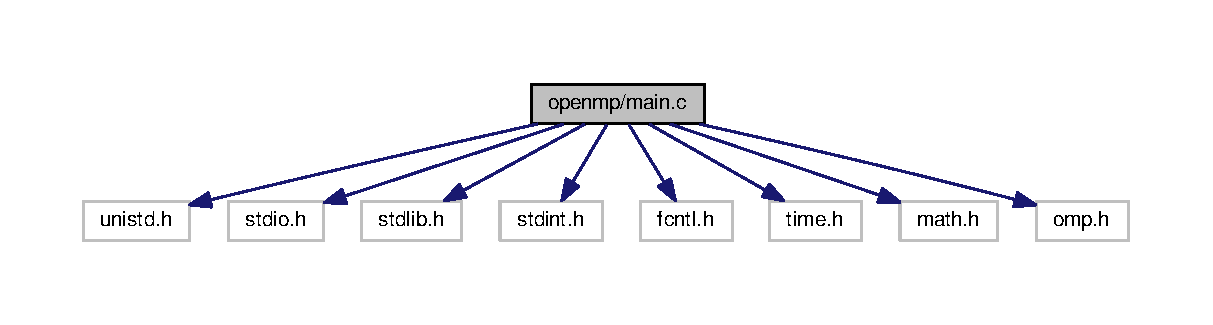
\includegraphics[width=350pt]{openmp_2main_8c__incl}
\end{center}
\end{figure}
\subsection*{Data Structures}
\begin{DoxyCompactItemize}
\item 
struct {\bf pulso}
\item 
struct {\bf tabla\+\_\+pulsos}
\end{DoxyCompactItemize}
\subsection*{Macros}
\begin{DoxyCompactItemize}
\item 
\#define {\bf C\+A\+N\+T\+\_\+\+P\+U\+L\+S\+OS}~800
\end{DoxyCompactItemize}
\subsection*{Functions}
\begin{DoxyCompactItemize}
\item 
void {\bf parsearpulsos} (int fd, {\bf tabla\+\_\+pulsos} $\ast$tablas[$\,$])
\item 
void {\bf calcularmedia} ({\bf tabla\+\_\+pulsos} $\ast$tablas[$\,$], float {\bf gates}[2][{\bf C\+A\+N\+T\+\_\+\+P\+U\+L\+S\+OS}][500][2])
\item 
void {\bf autocorrelacionar} (float {\bf gates}[2][{\bf C\+A\+N\+T\+\_\+\+P\+U\+L\+S\+OS}][500][2], float {\bf Rt}[2][500])
\item 
int {\bf main} (void)
\end{DoxyCompactItemize}


\subsection{Macro Definition Documentation}
\index{openmp/main.\+c@{openmp/main.\+c}!C\+A\+N\+T\+\_\+\+P\+U\+L\+S\+OS@{C\+A\+N\+T\+\_\+\+P\+U\+L\+S\+OS}}
\index{C\+A\+N\+T\+\_\+\+P\+U\+L\+S\+OS@{C\+A\+N\+T\+\_\+\+P\+U\+L\+S\+OS}!openmp/main.\+c@{openmp/main.\+c}}
\subsubsection[{C\+A\+N\+T\+\_\+\+P\+U\+L\+S\+OS}]{\setlength{\rightskip}{0pt plus 5cm}\#define C\+A\+N\+T\+\_\+\+P\+U\+L\+S\+OS~800}\label{openmp_2main_8c_adc8c780ab502933d827455d44da29d21}


\subsection{Function Documentation}
\index{openmp/main.\+c@{openmp/main.\+c}!autocorrelacionar@{autocorrelacionar}}
\index{autocorrelacionar@{autocorrelacionar}!openmp/main.\+c@{openmp/main.\+c}}
\subsubsection[{autocorrelacionar(float gates[2][C\+A\+N\+T\+\_\+\+P\+U\+L\+S\+OS][500][2], float Rt[2][500])}]{\setlength{\rightskip}{0pt plus 5cm}void autocorrelacionar (
\begin{DoxyParamCaption}
\item[{float}]{gates[2][\+C\+A\+N\+T\+\_\+\+P\+U\+L\+S\+O\+S][500][2], }
\item[{float}]{Rt[2][500]}
\end{DoxyParamCaption}
)}\label{openmp_2main_8c_a4b73fa1c29ba335698242ce10abe5cf6}
Calcula (de forma paralela) la autocorrelacion de cada pulso 
\begin{DoxyParams}{Parameters}
{\em gates} & arreglo de gates calculado a partir de la media \\
\hline
{\em Rt} & arreglo de valores de todos los gates autocorrelacionados por pulso\\
\hline
\end{DoxyParams}
\index{openmp/main.\+c@{openmp/main.\+c}!calcularmedia@{calcularmedia}}
\index{calcularmedia@{calcularmedia}!openmp/main.\+c@{openmp/main.\+c}}
\subsubsection[{calcularmedia(tabla\+\_\+pulsos $\ast$tablas[], float gates[2][C\+A\+N\+T\+\_\+\+P\+U\+L\+S\+OS][500][2])}]{\setlength{\rightskip}{0pt plus 5cm}void calcularmedia (
\begin{DoxyParamCaption}
\item[{{\bf tabla\+\_\+pulsos} $\ast$}]{tablas[$\,$], }
\item[{float}]{gates[2][\+C\+A\+N\+T\+\_\+\+P\+U\+L\+S\+O\+S][500][2]}
\end{DoxyParamCaption}
)}\label{openmp_2main_8c_a7f3d752870120b97691f1fbbab0485c9}
Calcula (de forma paralela) la media de los gates en la tabla de pulsos tablas y los almacena segun corresponda en el arreglo gates 
\begin{DoxyParams}{Parameters}
{\em tablas} & arreglo de punteros a structs donde se almacenan los valores parseados del archivo pulsos.\+iq \\
\hline
{\em gates} & arreglo de gates calculado a partir de la media\\
\hline
\end{DoxyParams}
\index{openmp/main.\+c@{openmp/main.\+c}!main@{main}}
\index{main@{main}!openmp/main.\+c@{openmp/main.\+c}}
\subsubsection[{main(void)}]{\setlength{\rightskip}{0pt plus 5cm}int main (
\begin{DoxyParamCaption}
\item[{void}]{}
\end{DoxyParamCaption}
)}\label{openmp_2main_8c_a840291bc02cba5474a4cb46a9b9566fe}
\index{openmp/main.\+c@{openmp/main.\+c}!parsearpulsos@{parsearpulsos}}
\index{parsearpulsos@{parsearpulsos}!openmp/main.\+c@{openmp/main.\+c}}
\subsubsection[{parsearpulsos(int fd, tabla\+\_\+pulsos $\ast$tablas[])}]{\setlength{\rightskip}{0pt plus 5cm}void parsearpulsos (
\begin{DoxyParamCaption}
\item[{int}]{fd, }
\item[{{\bf tabla\+\_\+pulsos} $\ast$}]{tablas[$\,$]}
\end{DoxyParamCaption}
)}\label{openmp_2main_8c_ad011f3aec555b84f682f21f9c9dbc4db}
Levanta el archivo pulsos.\+iq a memoria asignandolo a la tabla de pulsos ordenadamente segun corresponda 
\begin{DoxyParams}{Parameters}
{\em fd} & file descriptor del archivo pulsos.\+iq \\
\hline
{\em tablas} & arreglo de punteros a structs donde se almacenan los valores parseados del archivo pulsos.\+iq\\
\hline
\end{DoxyParams}

\section{procedural/main.c File Reference}
\label{procedural_2main_8c}\index{procedural/main.\+c@{procedural/main.\+c}}
{\ttfamily \#include $<$unistd.\+h$>$}\\*
{\ttfamily \#include $<$stdio.\+h$>$}\\*
{\ttfamily \#include $<$stdlib.\+h$>$}\\*
{\ttfamily \#include $<$stdint.\+h$>$}\\*
{\ttfamily \#include $<$fcntl.\+h$>$}\\*
{\ttfamily \#include $<$time.\+h$>$}\\*
{\ttfamily \#include $<$math.\+h$>$}\\*
{\ttfamily \#include $<$omp.\+h$>$}\\*
Include dependency graph for main.\+c\+:
\nopagebreak
\begin{figure}[H]
\begin{center}
\leavevmode
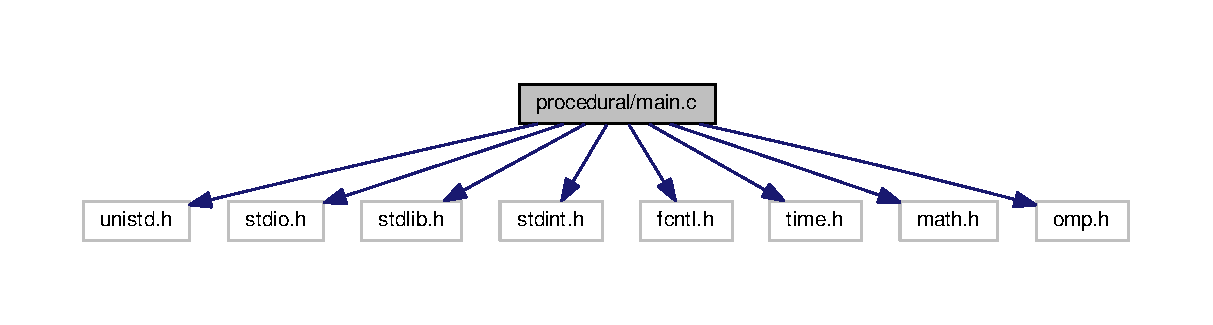
\includegraphics[width=350pt]{procedural_2main_8c__incl}
\end{center}
\end{figure}
\subsection*{Data Structures}
\begin{DoxyCompactItemize}
\item 
struct {\bf pulso}
\item 
struct {\bf tabla\+\_\+pulsos}
\end{DoxyCompactItemize}
\subsection*{Macros}
\begin{DoxyCompactItemize}
\item 
\#define {\bf C\+A\+N\+T\+\_\+\+P\+U\+L\+S\+OS}~800
\end{DoxyCompactItemize}
\subsection*{Functions}
\begin{DoxyCompactItemize}
\item 
void {\bf parsearpulsos} (int fd, {\bf tabla\+\_\+pulsos} $\ast$tablas[$\,$])
\item 
void {\bf calcularmedia} ({\bf tabla\+\_\+pulsos} $\ast$tablas[$\,$], float {\bf gates}[2][{\bf C\+A\+N\+T\+\_\+\+P\+U\+L\+S\+OS}][500][2])
\item 
void {\bf autocorrelacionar} (float {\bf gates}[2][{\bf C\+A\+N\+T\+\_\+\+P\+U\+L\+S\+OS}][500][2], float {\bf Rt}[2][500])
\item 
int {\bf main} (void)
\end{DoxyCompactItemize}


\subsection{Macro Definition Documentation}
\index{procedural/main.\+c@{procedural/main.\+c}!C\+A\+N\+T\+\_\+\+P\+U\+L\+S\+OS@{C\+A\+N\+T\+\_\+\+P\+U\+L\+S\+OS}}
\index{C\+A\+N\+T\+\_\+\+P\+U\+L\+S\+OS@{C\+A\+N\+T\+\_\+\+P\+U\+L\+S\+OS}!procedural/main.\+c@{procedural/main.\+c}}
\subsubsection[{C\+A\+N\+T\+\_\+\+P\+U\+L\+S\+OS}]{\setlength{\rightskip}{0pt plus 5cm}\#define C\+A\+N\+T\+\_\+\+P\+U\+L\+S\+OS~800}\label{procedural_2main_8c_adc8c780ab502933d827455d44da29d21}


\subsection{Function Documentation}
\index{procedural/main.\+c@{procedural/main.\+c}!autocorrelacionar@{autocorrelacionar}}
\index{autocorrelacionar@{autocorrelacionar}!procedural/main.\+c@{procedural/main.\+c}}
\subsubsection[{autocorrelacionar(float gates[2][C\+A\+N\+T\+\_\+\+P\+U\+L\+S\+OS][500][2], float Rt[2][500])}]{\setlength{\rightskip}{0pt plus 5cm}void autocorrelacionar (
\begin{DoxyParamCaption}
\item[{float}]{gates[2][\+C\+A\+N\+T\+\_\+\+P\+U\+L\+S\+O\+S][500][2], }
\item[{float}]{Rt[2][500]}
\end{DoxyParamCaption}
)}\label{procedural_2main_8c_a4b73fa1c29ba335698242ce10abe5cf6}
Calcula la autocorrelacion de cada pulso 
\begin{DoxyParams}{Parameters}
{\em gates} & arreglo de gates calculado a partir de la media \\
\hline
{\em Rt} & arreglo de valores de todos los gates autocorrelacionados por pulso\\
\hline
\end{DoxyParams}
\index{procedural/main.\+c@{procedural/main.\+c}!calcularmedia@{calcularmedia}}
\index{calcularmedia@{calcularmedia}!procedural/main.\+c@{procedural/main.\+c}}
\subsubsection[{calcularmedia(tabla\+\_\+pulsos $\ast$tablas[], float gates[2][C\+A\+N\+T\+\_\+\+P\+U\+L\+S\+OS][500][2])}]{\setlength{\rightskip}{0pt plus 5cm}void calcularmedia (
\begin{DoxyParamCaption}
\item[{{\bf tabla\+\_\+pulsos} $\ast$}]{tablas[$\,$], }
\item[{float}]{gates[2][\+C\+A\+N\+T\+\_\+\+P\+U\+L\+S\+O\+S][500][2]}
\end{DoxyParamCaption}
)}\label{procedural_2main_8c_a7f3d752870120b97691f1fbbab0485c9}
Calcula la media de los gates en la tabla de pulsos tablas y los almacena segun corresponda en el arreglo gates 
\begin{DoxyParams}{Parameters}
{\em tablas} & arreglo de punteros a structs donde se almacenan los valores parseados del archivo pulsos.\+iq \\
\hline
{\em gates} & arreglo de gates calculado a partir de la media\\
\hline
\end{DoxyParams}
\index{procedural/main.\+c@{procedural/main.\+c}!main@{main}}
\index{main@{main}!procedural/main.\+c@{procedural/main.\+c}}
\subsubsection[{main(void)}]{\setlength{\rightskip}{0pt plus 5cm}int main (
\begin{DoxyParamCaption}
\item[{void}]{}
\end{DoxyParamCaption}
)}\label{procedural_2main_8c_a840291bc02cba5474a4cb46a9b9566fe}
\index{procedural/main.\+c@{procedural/main.\+c}!parsearpulsos@{parsearpulsos}}
\index{parsearpulsos@{parsearpulsos}!procedural/main.\+c@{procedural/main.\+c}}
\subsubsection[{parsearpulsos(int fd, tabla\+\_\+pulsos $\ast$tablas[])}]{\setlength{\rightskip}{0pt plus 5cm}void parsearpulsos (
\begin{DoxyParamCaption}
\item[{int}]{fd, }
\item[{{\bf tabla\+\_\+pulsos} $\ast$}]{tablas[$\,$]}
\end{DoxyParamCaption}
)}\label{procedural_2main_8c_ad011f3aec555b84f682f21f9c9dbc4db}
Levanta el archivo pulsos.\+iq a memoria asignandolo a la tabla de pulsos ordenadamente segun corresponda 
\begin{DoxyParams}{Parameters}
{\em fd} & file descriptor del archivo pulsos.\+iq \\
\hline
{\em tablas} & arreglo de punteros a structs donde se almacenan los valores parseados del archivo pulsos.\+iq\\
\hline
\end{DoxyParams}

%--- End generated contents ---

% Index
\backmatter
\newpage
\phantomsection
\clearemptydoublepage
\addcontentsline{toc}{chapter}{Index}
\printindex

\end{document}
